\documentclass[11pt]{article}
\usepackage[margin=0.78in]{geometry}
\usepackage[T1]{fontenc}
\usepackage{amsmath,amssymb}
\usepackage{graphicx}
\graphicspath{{figures/}}
\usepackage{booktabs,longtable,array,multirow}
\usepackage{pdflscape}
\usepackage[hidelinks]{hyperref}
\usepackage{caption}
\usepackage{float}
\usepackage{xcolor}
\usepackage{enumitem}
\usepackage{microtype}
\usepackage{placeins}
\usepackage{tikz}
\usepackage{adjustbox}
\usetikzlibrary{arrows.meta,positioning,fit,calc}
\usepackage{tabularx}
\setlength{\parindent}{1.1em}
\setlength{\parskip}{0.30em}
\setlist[itemize]{leftmargin=1.7em,itemsep=0.2em,topsep=0.25em}
\newcommand{\PRISM}{PRISM-XAI}
\newcommand{\MAP}{MAP-XAI}
\newenvironment{interpretationbox}[1]{%
  \begin{quote}\small\noindent\textbf{#1}\ }{\end{quote}}
\newenvironment{cautionbox}{%
  \begin{quote}\small\noindent\textbf{Important caution.}\ }{\end{quote}}
\newenvironment{analysisbox}[1]{%
  \begin{quote}\small\noindent\textbf{Analysis focus.} #1\par\smallskip}{\end{quote}}
\title{PRISM-XAI: Extended Results, Analysis, and Reproducibility Companion}
\author{Extended technical supplement to the ICC manuscript}
\date{Evidence: M8 main matrix, M4 sensitivity, feasibility ladder, and privacy-release sweep}

\begin{document}
\maketitle

\begin{quote}\small
\textbf{Purpose and submission status.} This document is a self-contained technical supplement to the six-page ICC manuscript. It explains, compares, and interprets the complete v19 evidence rather than merely archiving plots and CSV files. The main paper does not depend on this document for any essential claim. At the time this package was prepared, no official ICC 2027 author instruction explicitly guaranteed that a separate supplementary file would be reviewed outside the six-page limit. Accordingly, this report is intended for author sharing, artifact/reproducibility review, or submission only if the final ICC 2027 system explicitly permits supplementary material. It can also be provided by the authors upon request.
\end{quote}


\tableofcontents
\clearpage

\begin{quote}\small
\textbf{Scope and organization.}
This supplement is designed to be self-contained with respect to the problem formulation, notation, privacy accounting, MAP-XAI and PRISM-XAI mechanisms, evaluation metrics, and experimental design. The technical foundations are established before the empirical evidence is presented. Each major result section states the analysis objective, reports the observed result, compares the proposed and reference methods, and discusses the corresponding implication and limitation. Exhaustive numerical tables are retained at the end for auditability and reproducibility.
\end{quote}

\part{Foundations, System Model, and Evaluation Context}

\section{Operational Problem and Motivation}
A short-term electricity-load forecaster produces a number: for example, the expected demand of a household or a group of households in the next time interval. An operator often needs more than that number. If demand is changing, the operator may want to know \emph{which factors drove the change}. A model explanation can answer that question by assigning an attribution value to each input feature. A positive or large-magnitude attribution indicates that the corresponding feature contributed strongly to the prediction under the chosen explanation method.

The difficulty studied here begins when explanations are no longer viewed as offline visualizations on a researcher's laptop. In a distributed smart-grid setting, explanations may have to travel from household-side or edge-side devices to an operator. Four constraints then interact:
\begin{enumerate}[leftmargin=2em]
\item \textbf{Communication is finite.} A full explanation vector sent from every endpoint at every slot consumes uplink resources.
\item \textbf{Explanations can reveal private behavior.} Feature attributions are derived from household data and can themselves act as an information channel.
\item \textbf{Privacy accumulates over time.} Even if one packet is individually private, repeated releases consume a finite privacy allowance over an operating horizon.
\item \textbf{Not every explanation is equally valuable.} A stale explanation during a critical grid condition may be more valuable than a fresh explanation during routine operation.
\end{enumerate}

This leads to the core systems question of the work: \emph{how can an edge system deliver explanations selectively, privately, and efficiently without pretending that communication, privacy, freshness, fidelity, and operational coverage can all be maximized at once?}

\begin{interpretationbox}{Core design principle.}
The work deliberately separates \emph{representation} from \emph{scheduling}. MAP-XAI decides how a private semantic explanation packet is represented. PRISM-XAI sits above that packetization layer and decides whether, when, from which endpoint, and at what semantic resolution an explanation should be transmitted.
\end{interpretationbox}

\section{Forecast Explanations and Attribution Representation}
Let endpoint $i$ observe a feature vector $\mathbf{x}_{i,t}\in\mathbb{R}^d$ at time slot $t$. A deployed forecasting model $f$ produces a prediction $\hat y_{i,t}$. An explanation method produces an attribution vector
\[
\boldsymbol{\phi}_{i,t}=\mathcal{E}(f,\mathbf{x}_{i,t})\in\mathbb{R}^d.
\]
The $j$th entry says how the $j$th feature contributes according to the explainer. The experiments use two explanation implementations, TreeSHAP and feature ablation, so the scheduler conclusions are not tied to one attribution algorithm.

For evaluation, the report also uses the word \textbf{oracle}. The oracle is the corresponding non-private explanation used offline as a reference for fidelity and driver-group agreement. It is not available to the online PRISM controller and is not used to decide whether a packet should be sent. The system is interested in changes in explanations rather than repeatedly sending a completely new vector. Let $t_i^-$ denote the most recent accepted explanation slot. The endpoint forms the explanation delta
\[
\Delta\boldsymbol{\phi}_{i,t}=\boldsymbol{\phi}_{i,t}-\boldsymbol{\phi}_{i,t_i^-}.
\]
This residual represents the change in the explanation since the last accepted update and is the semantic object that MAP-XAI protects and compresses.

\section{The two-layer architecture: MAP-XAI first, PRISM-XAI second}
\begin{figure}[htbp]
\centering
\resizebox{0.95\textwidth}{!}{%
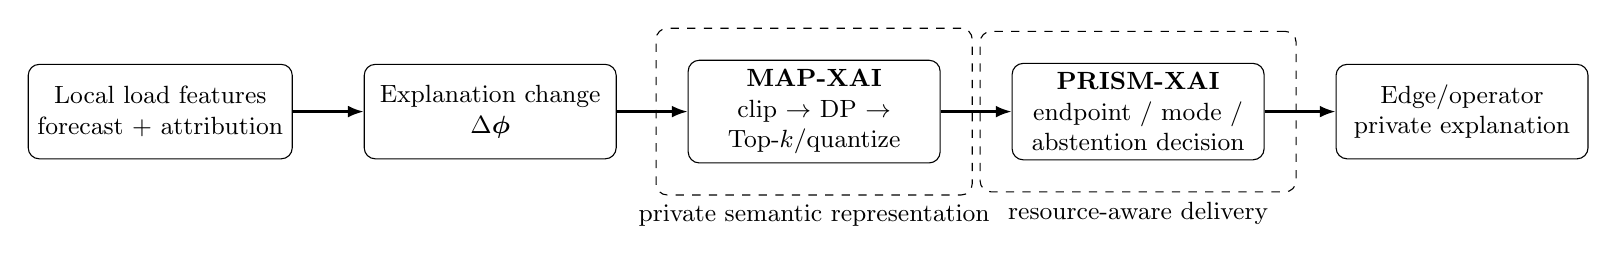
\begin{tikzpicture}[
node distance=8mm and 9mm,
box/.style={draw,rounded corners,align=center,minimum height=12mm,minimum width=32mm,font=\small},
layer/.style={draw,dashed,rounded corners,inner sep=4mm},
arr/.style={-{Latex[length=2mm]},thick}]
\node[box] (local) {Local load features\\forecast + attribution};
\node[box,right=of local] (delta) {Explanation change\\$\Delta\boldsymbol{\phi}$};
\node[box,right=of delta] (map) {\textbf{MAP-XAI}\\clip $\rightarrow$ DP $\rightarrow$\\Top-$k$/quantize};
\node[box,right=of map] (prism) {\textbf{PRISM-XAI}\\endpoint / mode /\\abstention decision};
\node[box,right=of prism] (operator) {Edge/operator\\private explanation};
\draw[arr] (local)--(delta);
\draw[arr] (delta)--(map);
\draw[arr] (map)--(prism);
\draw[arr] (prism)--(operator);
\node[layer,fit=(map),label={[font=\small]below:private semantic representation}] {};
\node[layer,fit=(prism),label={[font=\small]below:resource-aware delivery}] {};
\end{tikzpicture}}
\caption{Proposed two-layer architecture. MAP-XAI is a contribution of the paper and provides the private packetization layer. PRISM-XAI is the scheduling layer above it. Consequently, MAP-XAI-only is an internal restriction/ablation of the proposed stack, not an external competitor.}
\label{fig:tutorial-stack}
\end{figure}

The distinction in Fig.~\ref{fig:tutorial-stack} is important for interpreting the results. If full PRISM-XAI behaves similarly to MAP-XAI-only in a condition, that does not mean PRISM ``failed to beat a baseline.'' It means that the adaptive controller found little reason to depart from the valid packetization mode already supplied by the first contribution. Full PRISM is valuable because it has additional actions---including abstention, residual accumulation, alternative semantic modes, and gain-per-bit scheduling---when conditions justify them.

\section{MAP-XAI Semantic Packetization}
\subsection{Bounding Explanation Changes by Clipping}
The explanation delta is clipped to a fixed $\ell_2$ radius $C_i$:
\begin{equation}
\overline{\Delta\boldsymbol{\phi}}_{i,t}=
\frac{\Delta\boldsymbol{\phi}_{i,t}}
{\max\{1,\|\Delta\boldsymbol{\phi}_{i,t}\|_2/C_i\}}.
\label{eq:tutorial-clip}
\end{equation}
Clipping is not primarily a compression trick. It bounds sensitivity, which makes the subsequent privacy mechanism mathematically accountable. A very large explanation change is therefore scaled down rather than being allowed to create an arbitrarily sensitive release.

\subsection{Gaussian Perturbation Before \texorpdfstring{Top-$k$}{Top-k} Selection}
The clipped vector is privatized by adding Gaussian noise:
\begin{equation}
\widetilde{\Delta\boldsymbol{\phi}}_{i,t}=
\overline{\Delta\boldsymbol{\phi}}_{i,t}+\mathbf{n}_{i,t},
\qquad
\mathbf{n}_{i,t}\sim\mathcal{N}(0,\sigma_{i,t}^2 C_i^2\mathbf I).
\label{eq:tutorial-gauss}
\end{equation}
Only \emph{after} this private release is formed does MAP-XAI keep the largest coordinates and quantize their magnitudes. This ordering matters: Top-$k$ selection and quantization are post-processing of an already private output rather than operations performed on the raw private attribution vector.

\subsection{Semantic Packet Formation}
A packet mode can be described by the number of retained coordinates $k$, the quantization resolution $q$, and the Gaussian noise scale $\sigma$. The packet size used by the study has the form
\[
S_i(m)=S_0+k(\lceil\log_2 d\rceil+q+1),
\]
where the final bit records sign. The exact engineering point is less important than the principle: the system transmits \emph{selected semantic content}, not the entire attribution vector at full precision.

\begin{interpretationbox}{MAP-XAI contribution.}
MAP-XAI answers the question ``what is a privacy-accounted explanation packet?'' It is responsible for clipping, privatization, semantic selection, quantization, and cumulative privacy accounting. It does not decide the global wireless schedule by itself.
\end{interpretationbox}

\section{Differential Privacy and Horizon-Level Composition}
\subsection{Cumulative Privacy Loss Across Repeated Releases}
Differential privacy (DP) limits how much the released content can depend on one protected household under the stated adjacency model. The important issue here is \emph{repetition}. If a household sends many private explanation packets, the privacy cost of those releases must be composed. Treating each packet as if it were the only release would overstate privacy.

The implementation uses a R\'enyi-DP accountant. At an accounting order $\alpha$, one Gaussian release has cost
\[
\rho_{i,t}(\alpha)=\frac{\alpha}{2\sigma_{i,t}^2}.
\]
The costs add across admitted releases. At the end of the protected horizon, the composed budget is converted to an $(\epsilon_i,\delta_i)$ guarantee:
\begin{equation}
\epsilon_i(\delta_i)=\min_{\alpha}
\left\{\sum_t a_{i,t}\rho_{i,t}(\alpha)+
\frac{\log(1/\delta_i)}{\alpha-1}\right\}.
\label{eq:tutorial-rdp}
\end{equation}
Here $a_{i,t}=1$ when a private packet is exposed and zero otherwise.

\subsection{Interpretation of \texorpdfstring{$\epsilon$}{epsilon} in the Evaluated Privacy Regime}
The experiments use horizon budgets $\epsilon_{\max}\in\{8,16,32\}$ in the main M8 matrix, with $\delta=10^{-5}$. A larger $\epsilon$ permits a weaker privacy guarantee and typically allows lower noise for the same number of releases. It should not be read as a universal ``good'' or ``bad'' privacy score independent of the threat model. What matters for this study is that all private releases are charged to the same tracked horizon budget and no PRISM M8 run exceeds its configured budget.

\begin{cautionbox}
The theorem protects released packet \emph{content} under the stated add/remove household adjacency. Timing side channels are explicitly outside that formal guarantee. Also, the empirical attribute-attack AUC reported later is a diagnostic; it does not replace or define the DP guarantee.
\end{cautionbox}

\section{PRISM-XAI Scheduling Mechanism}
MAP-XAI gives the scheduler one privacy-valid semantic packet type. PRISM-XAI then asks whether transmitting a packet is worthwhile at the current slot.

\subsection{Freshness: Age of Explanation}
Let $A_{i,t}$ denote the Age of Explanation (AoX), the age of the last accepted explanation for endpoint $i$. Large AoX means the operator is relying on stale explanatory information. Public grid criticality can increase the value of freshness: a stale explanation during a critical state can matter more than the same staleness during routine operation.

\subsection{Value per bit}
For each feasible semantic mode $m$, the controller predicts an explanation-loss reduction $G_{i,t}(m)$ using only online-available information: AoX, public criticality, channel state, mode resolution, remaining privacy, and previously released privatized residual evidence. The scheduler never consults the non-private oracle explanation online. It then considers
\[
\Gamma_{i,t}(m)=\frac{G_{i,t}(m)}{S_i(m)},
\]
which is the expected explanation gain per transmitted bit.

\subsection{Abstention as a Scheduling Action}
PRISM can choose not to transmit. This is fundamental, because a privacy-aware system should not spend communication and privacy budget merely because a packet \emph{can} be sent. Unsent residual evidence is accumulated and decayed; a release becomes attractive only when the predicted semantic signal is large enough relative to the DP-noise floor.

\subsection{Feasibility and service guardrails}
A candidate transmission must fit the slot resource blocks, meet the deadline, and pass the privacy accountant. The scheduler also includes service guardrails for minimum critical-event coverage and Jain fairness. In the v19 M8 main matrix these are 5\% critical-event coverage and 0.88 minimum Jain fairness. The final empirical minima are higher: 5.98\% critical coverage and 0.972 Jain fairness across the 120 PRISM runs.

\section{Illustrative Endpoint-Level Scheduling Sequence}
Consider an endpoint whose most recent accepted explanation is becoming stale. At the same time, a public indicator marks the zone as critical.
\begin{enumerate}[leftmargin=2em]
\item The local explainer computes the current attribution vector and the change relative to the last accepted explanation.
\item MAP-XAI clips that change, adds Gaussian noise, and forms candidate semantic packets only from the privatized vector.
\item The privacy accountant checks whether another private release fits inside the endpoint's remaining horizon budget.
\item PRISM evaluates whether the packet is worth its transmitted bits, accounting for AoX, criticality, channel conditions, fairness, residual signal, and energy/privacy prices.
\item If the packet is not valuable enough, PRISM abstains and carries residual evidence forward. If it is valuable and feasible, the scheduler may transmit the MAP-XAI packet or another allowed semantic mode.
\item At the operator side, the received private explanation is reconstructed and evaluated. The experiment then asks both \emph{explanation questions} (e.g., Top-$K$ agreement) and \emph{operational questions} (e.g., was a critical event covered and was the driver group correct?).
\end{enumerate}
The important point is that privacy loss, communication cost, explanation fidelity, and operational coverage arise at different stages. Later, the feasibility ladder will isolate these stages experimentally.

\section{Evaluation Metrics}
Interpreting the system through a single metric is insufficient because communication, privacy, freshness, fidelity, and operational service are coupled. The study therefore reports several metric families.

\subsection{Explanation-quality metrics}
\begin{center}
\small
\begin{tabularx}{\textwidth}{>{\bfseries}p{0.22\textwidth} X p{0.18\textwidth}}
\toprule
Metric & Interpretation & Direction \\
\midrule
Cosine similarity & Directional alignment between the oracle zone-level attribution vector and the reconstructed private attribution vector. Near 1 means similar direction; near 0 means little alignment; negative values indicate opposing direction. & Higher is better. \\
Spearman $\rho$ & Agreement in feature ranking rather than absolute magnitudes. & Higher is better. \\
Top-$K$ overlap & Fractional agreement among the most important features. The experiment's random reference is 0.25. & Higher is better. \\
Top-$K$ sign agreement & Whether the signs of the important attributions agree. Around 0.5 is weak/sign-like-chance behavior. & Higher is better. \\
Hierarchical distortion & Relative reconstruction error after aggregating household explanations to zones. & Lower is better. \\
Collapse rate & Fraction of evaluation steps whose mean cosine similarity is below 0.5; this is the generator's explicit collapse criterion. & Lower is better. \\
Max collapse duration & Longest consecutive run of steps satisfying the collapse criterion. & Lower is better. \\
\bottomrule
\end{tabularx}
\end{center}

\subsection{Operational metrics}
A critical event is counted at the zone level. Criticality is generated from public forecast behavior: a zone is marked critical when its predicted level exceeds the 80th-percentile calibration threshold for that zone or its absolute prediction ramp exceeds the 90th-percentile calibration ramp threshold. This is therefore a reproducible operational stress proxy, not a label claiming that an actual grid emergency occurred. The generator regards a critical event as \emph{covered} only when the mean AoX for the zone is at most eight slots and the mean public certified-quality state is at least 0.10. Agreement means that the oracle and reconstructed explanations identify the same driver group, where the 12 features are partitioned into four fixed groups and the group with largest summed absolute attribution is treated as the dominant driver.
\begin{center}
\small
\begin{tabularx}{\textwidth}{>{\bfseries}p{0.22\textwidth} X p{0.18\textwidth}}
\toprule
Metric & Interpretation & Direction \\
\midrule
Critical-event coverage & Covered critical events divided by all critical events. It answers ``how often did the system have an explanation fresh/reliable enough to act on?'' & Higher is better. \\
Critical-event recall & Correctly handled critical events divided by all critical events. In the generator this equals operational agreement over all critical events. & Higher is better. \\
Intervention precision & Correct critical interventions divided by correct critical interventions plus actionable false interventions in noncritical periods. & Higher is better. \\
Abstention rate & One minus critical coverage. It quantifies deliberate non-service. & Lower is better only if other constraints are unchanged. \\
False intervention rate & Actionable false decisions in noncritical periods divided by noncritical events. & Lower is better. \\
Conditional error accepted & Reconstruction error only on critical events that passed the online coverage certificate. & Lower is better. \\
\bottomrule
\end{tabularx}
\end{center}

\subsection{Communication, freshness, fairness, and privacy metrics}
\begin{center}
\small
\begin{tabularx}{\textwidth}{>{\bfseries}p{0.22\textwidth} X p{0.18\textwidth}}
\toprule
Metric & Interpretation & Direction \\
\midrule
Transmitted kbit & Total explanation traffic sent over the evaluation horizon. & Lower is better, subject to service. \\
Bits per correct intervention & Communication spent per correctly handled critical event. & Lower is better. \\
Delivery ratio / deadline miss & Whether scheduled packets are delivered within the simulated link/deadline model. & Higher delivery, lower misses. \\
Mean / P95 AoX & Average and tail staleness of accepted explanations. & Lower is fresher. \\
Energy & Modeled transmission energy. & Lower is better. \\
Jain fairness & How uniformly service is distributed across endpoints; one is perfectly equal. & Higher is better. \\
Spent $\epsilon$ & Composed privacy cost over the horizon. & Must stay within the configured budget. \\
Attack AUC & Cross-validated ability of a logistic attacker to infer the stored private endpoint attribute from reconstructed-explanation aggregates; values are oriented to be at least 0.5. & Lower is empirically preferable; not the formal DP guarantee. \\
\bottomrule
\end{tabularx}
\end{center}

\begin{interpretationbox}{Interpretation of recall and precision.}
A selective policy can abstain often, which lowers coverage and recall, while still making its accepted interventions more precise. Therefore ``high precision'' must never be presented without coverage/recall, and ``low traffic'' must never be presented without the service level achieved at that traffic.
\end{interpretationbox}

\section{Datasets and experimental design}
The main experiments use two real electricity-load datasets. OPSD contributes nine endpoints grouped into three synthetic zones. UCI ElectricityLoadDiagrams20112014 contributes 32 endpoints grouped into four synthetic zones. The zone hierarchy is synthetic in both cases; this is an evaluation abstraction, not a claim that the data supply a physical feeder topology. Each model uses 12 lag, rolling-statistic, and calendar features. The deployed tree forecaster has RMSE/MAE 0.926/0.545 on OPSD and 1.289/0.221 on UCI. Scheduler choice does not retrain the predictor.

The wireless abstraction uses eight 180 kHz resource blocks, 1 ms slots, a 5 ms deadline, a 3.5 GHz carrier, path loss, correlated shadowing, small-scale fading, edge delay, and bursty failures. It is a reproducible scheduler-level stress model, not a link-level field trial.

The main M8 experiment uses 512 evaluation slots after 96 calibration slots, $\epsilon_{\max}\in\{8,16,32\}$, $\delta=10^{-5}$, at most eight private releases per endpoint, and ten paired random seeds. The M4 sensitivity study repeats the design with a four-release cap. The full matrix is
\[
2\text{ datasets}\times2\text{ XAI methods}\times3\text{ privacy budgets}\times6\text{ schedulers}\times10\text{ seeds}=720\text{ runs}.
\]

\section{Calibration and Evaluation Horizon}

The main experiment uses an initial calibration period of 96 slots followed by 512 evaluation slots. The calibration interval estimates quantities required by the online scheduler, including characteristic explanation-residual scales and related calibration statistics. Performance metrics are computed only over the subsequent evaluation horizon:

\[
\underbrace{96\text{ calibration slots}}_{\text{parameter calibration}}
\quad\longrightarrow\quad
\underbrace{512\text{ evaluation slots}}_{\text{scheduler evaluation}}.
\]

This separation prevents observations used to establish scheduler calibration from being reused as evaluation samples.

\section{Comparison Policies}

The evaluation contains four external reference policies and one restricted internal configuration of the proposed framework.

\paragraph{Periodic fixed-DP.}
This policy transmits private explanations according to a regular schedule without adapting the transmission decision to explanation value, channel quality, or explanation freshness. It represents a conventional periodic private-explanation service.

\paragraph{Channel fixed-DP.}
This policy prioritizes favorable wireless-channel opportunities. It isolates the benefit obtainable when communication conditions dominate the scheduling decision, without explicitly accounting for semantic explanation value.

\paragraph{AoX fixed-DP.}
This policy prioritizes endpoints with large Age of Explanation (AoX), where AoX measures the elapsed time since the most recent accepted explanation. The method therefore emphasizes freshness and service frequency. It represents an aggressive explanation-delivery policy and is expected to obtain relatively high critical-event coverage at the expense of increased communication.

\paragraph{Joint full packet.}
This policy jointly schedules full, uncompressed private explanation packets. It evaluates whether transmitting richer explanations without semantic packet reduction provides sufficient fidelity benefit to justify the additional communication cost.

\paragraph{MAP-XAI-only.}
MAP-XAI-only is an internal restriction of the proposed framework rather than an external baseline. It retains the proposed privacy-accounted semantic packetization mechanism but removes the additional adaptive scheduling behavior of PRISM-XAI. The comparison

$$
\text{MAP-XAI-only}
\quad\longrightarrow\quad
\text{MAP-XAI + PRISM-XAI}
$$

therefore isolates the incremental contribution of PRISM's scheduling layer after semantic packetization is already available.

This distinction is important because similarity between MAP-XAI-only and PRISM-XAI under a particular operating condition does not imply that the complete system has failed to outperform an external competitor. Instead, it may indicate that the scheduler has identified MAP-XAI packetization itself as the appropriate operating mode under that condition.

\section{Paired Statistical Protocol}

All primary statistical comparisons use matched random seeds. For a fixed dataset, explanation method, and privacy budget, PRISM-XAI and each reference policy are evaluated using the same ten stochastic seeds so that the policies experience matched simulated system and wireless conditions.

For each metric, paired differences are computed seed by seed and summarized with a 95\% confidence interval of the mean paired difference. A result favors PRISM-XAI only when the complete interval lies on the favorable side of zero; an interval containing zero is reported as a tie. This criterion is more conservative than ranking methods solely by sample means.

\part{ Experimental Evidence}

\section{Experimental Integrity and Validation}

Performance comparisons are meaningful only if the underlying run matrix, privacy accounting, paired traces, and reported metrics are internally consistent. We therefore validate the experimental outputs before interpreting algorithmic performance.

The validation procedure verifies that the expected experiment configurations are present, that scheduler comparisons use matching dataset/XAI/privacy/seed combinations, that run identifiers are unique, that the underlying trace provenance is consistent, and that cumulative privacy expenditure remains within the configured horizon-level budget.

The main M8 experiment contains the intended 720-run matrix. Across the 120 PRISM-XAI runs, no cumulative privacy-budget violation is observed. The minimum critical-event coverage is 0.0598, above the configured 5\% floor, and the minimum Jain delivery fairness is 0.9719, above the configured 0.88 guardrail.

The aggregate generator validation flag requires one additional clarification. For both M8 and M4, this aggregate flag is reported as false because the validation script also expects an optional ablation-control output. The corresponding v19 M8/M4 ablation CSV files are empty. Dataset-level validation, run-key uniqueness, privacy accounting, and trace-provenance checks nevertheless pass.

Accordingly, the false aggregate flag does not indicate failure of the primary v19 experiment or violation of the privacy budget. It records the absence of an optional ablation artifact. We retain this status explicitly rather than substituting an older v18 ablation result, since mixing experimental versions would compromise the consistency of the v19 evidence base.

The subsequent analysis therefore uses only the verified v19 M8 results, the separately identified M4 sensitivity experiment, and the independently generated feasibility-ladder and privacy--release diagnostic studies.



% In the preamble:
% \usepackage{adjustbox}
% \usepackage{booktabs}

\begin{table*}[t]
\centering
\caption{v19 result-bundle validation metadata. The statistical M4/M8 bundles have a false aggregate flag only because the optional ablation-control file is absent; all dataset validation, key uniqueness, and trace provenance checks pass. The engineering verification is explicitly not used as a statistical paper result.}
\label{tab:validation}

\scriptsize
\setlength{\tabcolsep}{3pt}
\renewcommand{\arraystretch}{1.08}

\begin{adjustbox}{max width=\textwidth}
\begin{tabular}{llccccc p{7.0cm}}
\toprule
Bundle
& Mode
& Data valid
& Keys unique
& Trace prov.
& Ablation ctl.
& Overall
& Note \\
\midrule

M8 statistical matrix
& full
& True
& True
& True
& False
& False
& Full paired real-data experiment matrix. \\

M4 sensitivity matrix
& full
& True
& True
& True
& False
& False
& Full paired real-data experiment matrix. \\

Engineering verification
& verification
& True
& True
& True
& True
& True
& Engineering verification only; not used as a statistical paper result. \\

\bottomrule
\end{tabular}
\end{adjustbox}
\end{table*}

The scheduler does not alter the deployed forecaster. Table~\ref{tab:forecast} therefore shows identical forecasting error for the two XAI implementations within each dataset. OPSD has RMSE 0.926 and MAE 0.545; UCI has RMSE 1.289 and MAE 0.221. This separation is useful: differences reported later come from explanation representation and scheduling rather than from retraining a different predictor for each communication policy.

% In the preamble:
% \usepackage{adjustbox}
% \usepackage{booktabs}

\begin{table*}[t]
\centering
\caption{Forecast error used by the v19 experiments, averaged across paired seeds and schedulers. The scheduler does not change the deployed forecaster.}
\label{tab:forecast}

\scriptsize
\setlength{\tabcolsep}{6pt}
\renewcommand{\arraystretch}{1.08}

\begin{adjustbox}{max width=0.65\textwidth}
\begin{tabular}{llrr}
\toprule
Dataset & XAI method & RMSE & MAE \\
\midrule

OPSD & TreeSHAP & 0.926 & 0.545 \\
OPSD & feature\_ablation & 0.926 & 0.545 \\
UCI & TreeSHAP & 1.289 & 0.221 \\
UCI & feature\_ablation & 1.289 & 0.221 \\

\bottomrule
\end{tabular}
\end{adjustbox}
\end{table*}


\section{Main v19 M8 Results: Operating-Point Trade-off}

\subsection*{Representative Conditions Before Macro-Averaging}
At $\epsilon_{\max}=8$, averaged over the two XAI implementations and ten paired seeds, OPSD PRISM uses 104.6 kbit, covers 7.1\% of critical events, correctly handles 2.8\% of all critical events, reaches intervention precision 0.306, and spends about 9.7 kbit per correct intervention. AoX fixed-DP uses 1,560.6 kbit, covers 27.9\%, recalls 12.0\%, has precision 0.202, and spends 34.9 kbit per correct intervention. On UCI, PRISM uses 376.2 kbit at 9.0\% coverage, 4.4\% recall, 0.493 precision, and 10.7 kbit/correct, while AoX fixed-DP uses 5,300.2 kbit at 99.7\% coverage, 45.6\% recall, 0.362 precision, and 14.1 kbit/correct. These examples show the trade-off immediately: PRISM is not serving the same number of events more cheaply; it is choosing a much more selective service point and spending its scarce private transmissions more efficiently.
\subsection{Communication and energy efficiency}
The first and most stable result is communication efficiency. Across the 12 matched dataset/XAI/privacy conditions, PRISM transmits only 242.5 kbit on average, compared with 4,645.2 kbit for periodic fixed-DP, 4,573.8 kbit for channel fixed-DP, 4,643.6 kbit for AoX fixed-DP, and 1,655.4 kbit for joint full-packet scheduling. \MAP{}-only is essentially at the same communication scale (243.7 kbit), which is expected because it is our restricted packetization mode inside the full design rather than an external competitor.

Condition-by-condition rather than by a ratio of macro means, PRISM reduces traffic by 94.6\% relative to each of the three fixed-DP schedulers and by 79.4\% relative to joint full-packet scheduling. The reduction is not confined to one favorable dataset or privacy budget: paired 95\% confidence intervals show lower traffic in all 48 external-baseline comparisons. Energy follows the same pattern because transmission dominates the modeled communication energy: PRISM averages 36.4 mJ versus roughly 685--698 mJ for fixed-DP and 248.7 mJ for joint full-packet scheduling.

\begin{table}[htbp]\centering\small
\caption{Condition-wise efficiency reduction of PRISM relative to each external reference. Percentages are computed within each matched dataset/XAI/privacy condition and then averaged.}
\label{tab:reduction-scorecard}
\begin{tabular}{lrrrrr}
\toprule
Reference & Traffic red. & Min & Max & Energy red. & bit/correct red. \\
\midrule
Periodic fixed-DP & 94.6\% & 92.8\% & 98.0\% & 94.6\% & 84.4\% \\
Channel fixed-DP & 94.6\% & 92.8\% & 98.0\% & 94.6\% & 86.9\% \\
AoX-aware fixed-DP & 94.6\% & 92.8\% & 98.0\% & 94.6\% & 46.8\% \\
Joint full packet & 79.4\% & 49.1\% & 94.1\% & 79.4\% & 54.2\% \\
\bottomrule
\end{tabular}
\end{table}

\begin{figure}[htbp]
\centering
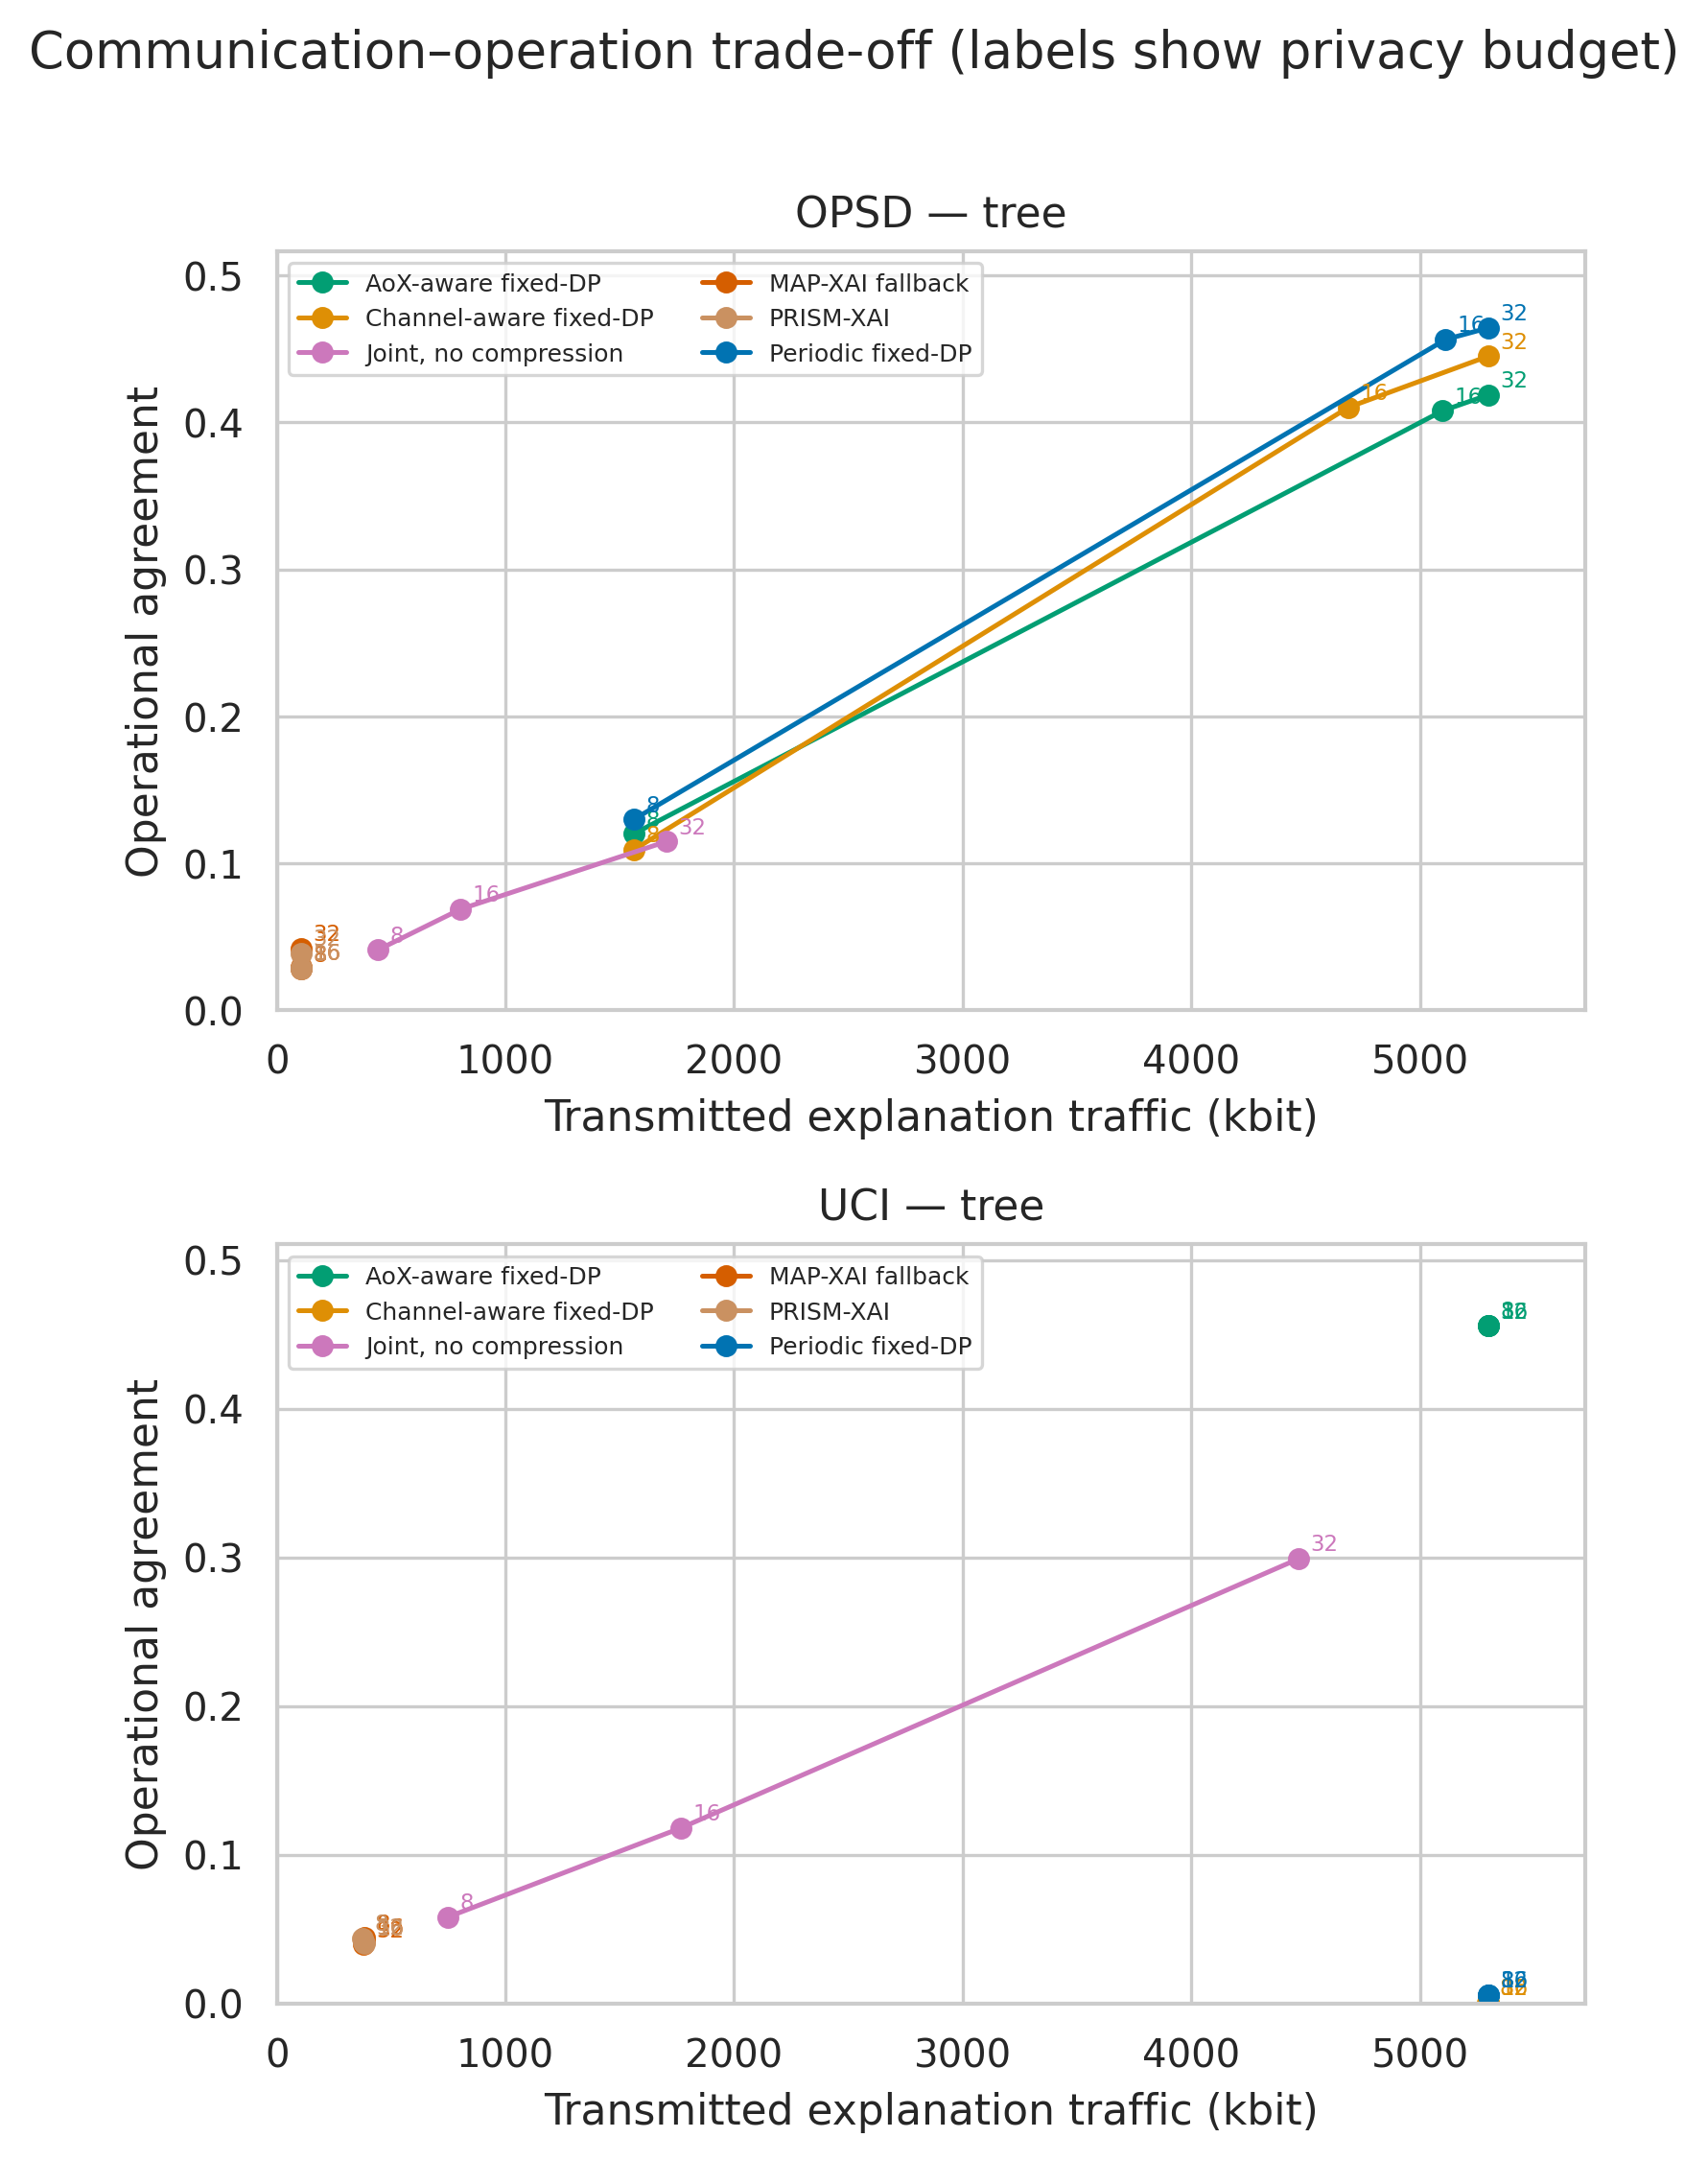
\includegraphics[width=.76\linewidth]{original_v19_M8_pareto_bits_fidelity.png}
\caption{Original v19 M8 communication--operation trade-off. The proposed modes occupy the low-traffic region. AoX fixed-DP reaches much higher operational agreement, especially on UCI, by transmitting far more frequently. The figure therefore visualizes an efficiency/service trade-off rather than an unconditional dominance result.}
\label{fig:orig-pareto}
\end{figure}

The low traffic also translates into a better communication cost per correct intervention. PRISM averages 9,987 bits per correct intervention; \MAP{}-only averages 9,960. AoX fixed-DP is 23,572 and joint full packet 25,498, while periodic and channel fixed-DP become extremely inefficient because many transmissions do not translate into correct intervention decisions. In the paired analysis, PRISM has significantly lower bits per correct intervention in 45 of the 48 external-baseline settings. The three non-wins are statistical ties, not significant losses.


\subsection{The cost of selectivity: coverage and recall}
Communication savings are purchased by selective service. PRISM's macro critical-event coverage is 0.078 and its critical-event recall is 0.037. Joint full-packet scheduling covers 0.248 and recalls 0.117; AoX fixed-DP covers 0.875 and recalls 0.386. These numbers must remain visible whenever the traffic reduction is discussed. In particular, the AoX baseline is intentionally aggressive: it keeps serving critical conditions and therefore achieves the strongest recall, but at approximately nineteen times PRISM's macro traffic.

The more favorable operational metric for the proposed stack is \emph{precision}. PRISM's macro intervention precision is 0.510 and \MAP{}-only reaches 0.538, compared with 0.226 for periodic fixed-DP, 0.189 for channel fixed-DP, 0.285 for AoX fixed-DP, and 0.314 for joint full packet. Across the 48 external paired comparisons, PRISM precision is significantly higher in 38 and tied in 10; it is never significantly lower. The intended reading is therefore: the M8 policy intervenes less often, but its accepted interventions are substantially more selective.

This is also visible in the false-intervention rate: PRISM is 0.020 and \MAP{}-only 0.019, versus 0.136--0.501 across the external references. The macro false-activation metric is saturated at 1.0 for all four external references and therefore has limited discriminative value in this experiment; it should be read together with false interventions, driver mismatch, precision, and coverage rather than in isolation.


\begin{table}[htbp]\centering\small
\caption{Dataset-level v19 M8 scorecard, averaged over two XAI methods, three privacy budgets, and ten seeds per condition.}
\label{tab:dataset-scorecard}
\resizebox{\textwidth}{!}{%
\begin{tabular}{llrrrrrrrr}
\toprule
Data & Method & kbit & Top-K & Cosine & Crit. cov. & Recall & Precision & bit/correct & Jain \\
\midrule
OPSD & Periodic fixed-DP & 3991.0 & 0.245 & -0.014 & 0.754 & 0.350 & 0.232 & 28,525 & 1.000 \\
OPSD & Channel fixed-DP & 3849.1 & 0.270 & -0.010 & 0.666 & 0.321 & 0.245 & 33,511 & 0.948 \\
OPSD & AoX-aware fixed-DP & 3986.9 & 0.247 & -0.015 & 0.752 & 0.316 & 0.209 & 33,038 & 0.999 \\
OPSD & Joint full packet & 982.5 & 0.259 & -0.022 & 0.153 & 0.075 & 0.246 & 33,366 & 0.976 \\
OPSD & MAP-XAI-only (ours) & 106.2 & 0.302 & 0.183 & 0.071 & 0.033 & 0.401 & 8,449 & 0.990 \\
OPSD & PRISM-XAI (ours) & 105.6 & 0.317 & 0.198 & 0.071 & 0.032 & 0.379 & 8,649 & 0.990 \\
\midrule
UCI & Periodic fixed-DP & 5299.3 & 0.260 & 0.009 & 0.011 & 0.006 & 0.219 & 1,385,471 & 0.999 \\
UCI & Channel fixed-DP & 5298.5 & 0.257 & 0.001 & 0.001 & 0.000 & 0.133 & 4,967,504 & 0.526 \\
UCI & AoX-aware fixed-DP & 5300.2 & 0.262 & 0.001 & 0.997 & 0.456 & 0.361 & 14,107 & 0.999 \\
UCI & Joint full packet & 2328.3 & 0.260 & 0.012 & 0.344 & 0.158 & 0.382 & 17,629 & 0.954 \\
UCI & MAP-XAI-only (ours) & 381.3 & 0.229 & 0.056 & 0.085 & 0.042 & 0.675 & 11,472 & 0.992 \\
UCI & PRISM-XAI (ours) & 379.4 & 0.240 & 0.012 & 0.086 & 0.042 & 0.640 & 11,325 & 0.992 \\
\bottomrule
\end{tabular}}
\end{table}

\subsection{Explanation fidelity: improved structure, but not a solved problem}
The explanation metrics tell a more nuanced story. PRISM's macro Top-$K$ overlap is 0.279 and \MAP{}-only is 0.265, compared with a random Top-$K$ reference of 0.25. External references cluster between 0.252 and 0.264. Paired confidence intervals therefore show that Top-$K$ is usually a statistical tie: against external references PRISM is higher in eight settings, tied in 37, and lower in three. Accordingly, the main paper does not claim universal Top-$K$ superiority.

Other explanation metrics are more favorable. PRISM has mean cosine 0.105 and Spearman 0.072; \MAP{}-only has 0.119 and 0.084. External methods are approximately zero or slightly negative in cosine and Spearman. Top-$K$ sign agreement is 0.565 for PRISM and 0.573 for \MAP{}-only versus about 0.50--0.51 externally. Hierarchical distortion falls to 12.07 for PRISM and 11.17 for \MAP{}-only, compared with 131 for joint full packet and roughly 241--263 for the fixed-DP schedulers. Thus the proposed representation retains more directional and hierarchical structure even when exact Top-$K$ identity remains difficult under cumulative DP.

At the same time, collapse remains frequent: the macro collapse rate is 0.954 for PRISM and 0.961 for \MAP{}-only, with long maximum collapse durations. This is not hidden. It is consistent with the later feasibility ladder, which shows that the main destruction of attribution signal occurs at the repeated private-release step. The proposed scheduler can decide when a release is worth sending, but it cannot reconstruct information already erased by DP noise.


\begin{figure}[htbp]
\centering
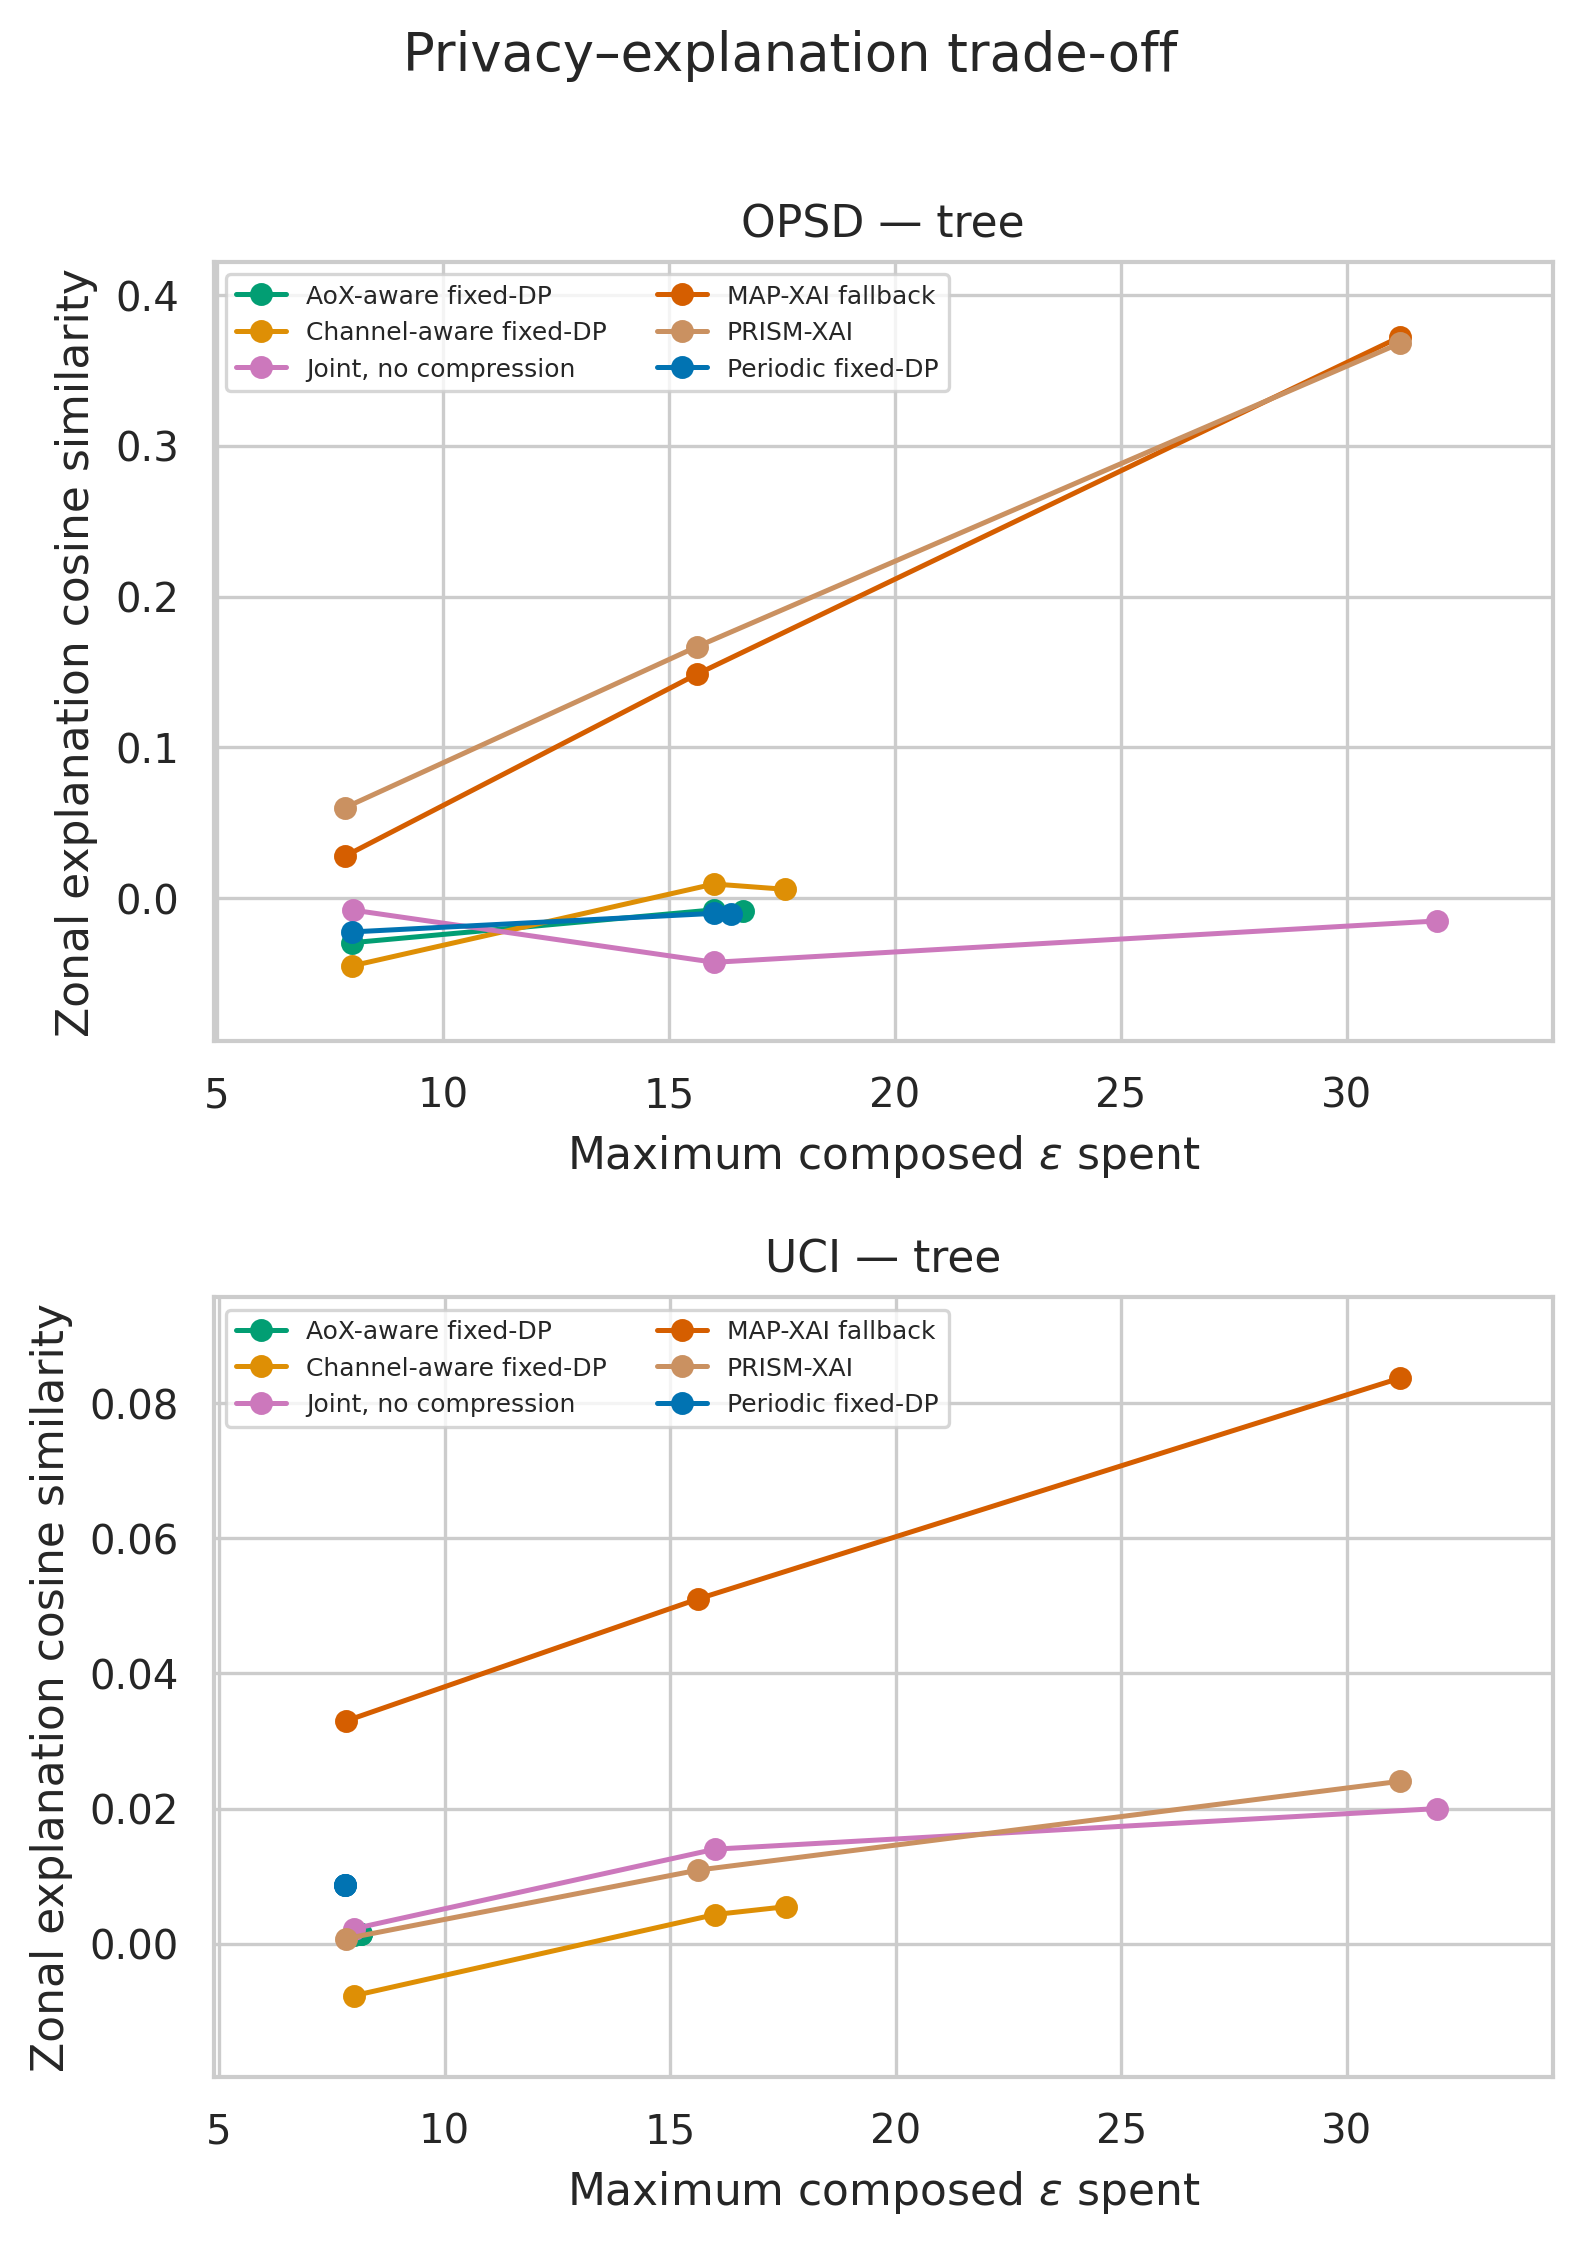
\includegraphics[width=.86\linewidth]{original_v19_M8_privacy_fidelity.png}
\caption{Original v19 M8 privacy--fidelity plot. Larger privacy budgets improve the proposed modes most clearly on OPSD. UCI remains much more difficult, showing that a larger $\epsilon$ budget helps but does not remove the dataset-dependent privacy/fidelity limitation.}
\label{fig:orig-privacy}
\end{figure}

\subsection{Wireless reliability, latency, freshness, and fairness}
The communication savings do not come from accepting a worse radio delivery ratio. Delivery ratios stay in a narrow range across methods: approximately 0.944--0.950. Deadline miss rates also remain around 5--6\%, and mean latencies stay near 2.3--2.4 ms. The paired tests show deadline-miss differences are overwhelmingly ties. In other words, the main difference among policies is how often they choose to transmit, not whether the simulated link suddenly becomes more reliable for PRISM.

The price of selective release appears in Age of Explanation (AoX). PRISM and \MAP{}-only have mean AoX around 226 slots, compared with 23 for AoX fixed-DP, 27 for periodic fixed-DP, 100 for channel fixed-DP, and 158 for joint full packet. This is exactly what the design implies: a policy with only eight private releases per endpoint over the evaluation horizon cannot keep explanations uniformly fresh. The scientific question is therefore whether those scarce releases are spent on higher-value events, not whether PRISM can simultaneously achieve the freshness of an almost-always-transmitting AoX policy.

Fairness remains high. PRISM's macro Jain index is 0.991 and \MAP{}-only is 0.991. Periodic and AoX fixed-DP are even closer to 1.0 because they transmit much more uniformly and frequently; channel fixed-DP falls to 0.737 overall and much lower on UCI, indicating that channel opportunism can starve endpoints. Joint full packet reaches 0.965. The fair conclusion is not that PRISM has the highest fairness of every method, but that it retains near-uniform endpoint service despite an extremely sparse private-release budget.


\begin{figure}[htbp]
\centering
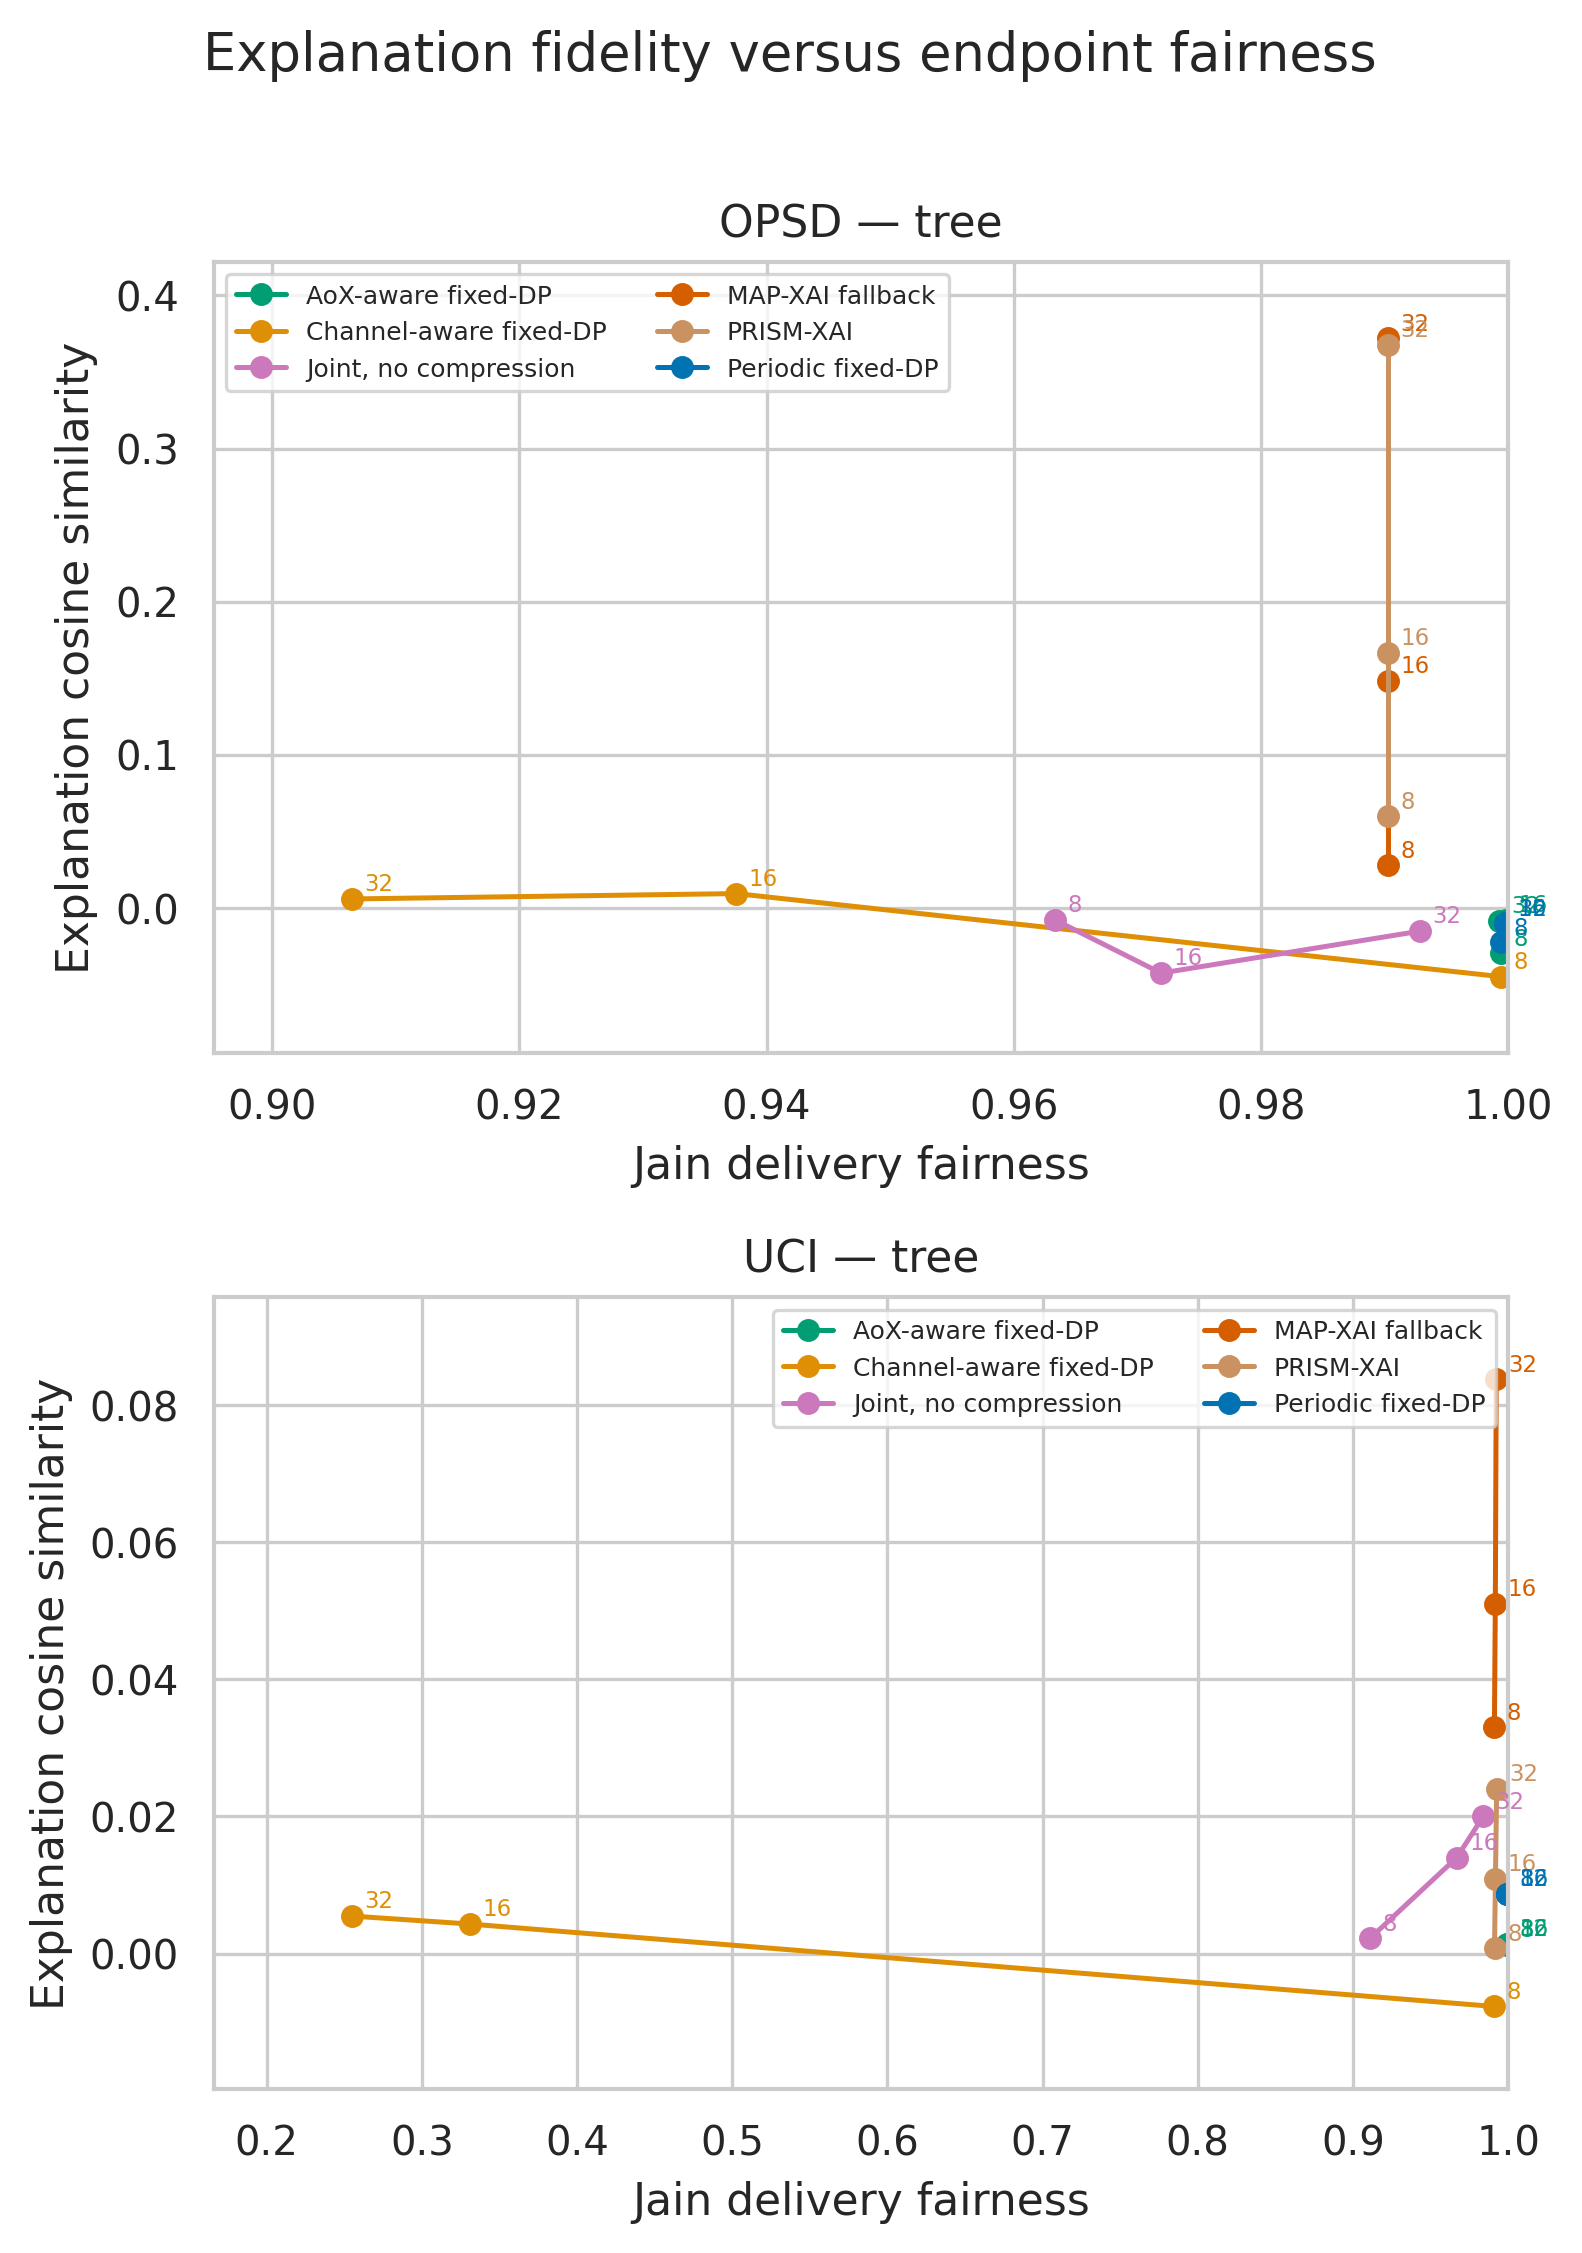
\includegraphics[width=.86\linewidth]{original_v19_M8_fairness_reliability.png}
\caption{Original v19 M8 fairness--fidelity plot. PRISM and MAP-XAI-only remain close to Jain fairness one. The channel-driven policy can trade fairness away, especially on UCI, which motivates reporting endpoint fairness alongside communication and fidelity.}
\label{fig:orig-fairness}
\end{figure}

\subsection{Privacy accounting and empirical attack diagnostic}
The formal privacy claim rests on the RDP accountant and the configured horizon budget. PRISM has no budget violations across its 120 M8 runs, and its maximum spent $\epsilon$ remains below each configured budget. Its mean and maximum number of private releases per endpoint are both eight, matching the M8 policy. In contrast, the external baselines release many more private packets and often drive a nonzero fraction of endpoints to the accountant's exhaustion boundary; joint full-packet scheduling reaches exhaustion fraction 1.0 in the macro table.

The empirical attribute-attack AUC deserves separate treatment. PRISM and \MAP{}-only are around 0.71, while external references are roughly 0.66--0.69. Therefore the report does \emph{not} claim that PRISM has the lowest empirical attack AUC. A plausible interpretation is that selective semantic packets can be more informative conditional on being sent, but the present experiment does not isolate the cause. The formal content-privacy guarantee is the DP accountant, not this attack metric. For deployment, both accountant guarantees and empirical leakage diagnostics should be reported.


\section{Dataset-by-dataset analysis}
The aggregate result hides an important difference between OPSD and UCI. The same communication strategy behaves similarly in traffic and fairness, but not in explanation reconstruction.

\subsection{OPSD: stronger explanation recovery at low traffic}
On OPSD, PRISM averages 105.6 kbit, Top-$K$ 0.317, cosine 0.198, critical coverage 0.071, recall 0.032, precision 0.379, and Jain fairness 0.990. \MAP{}-only is almost identical in traffic and coverage but has Top-$K$ 0.302 and cosine 0.183. The fixed-DP references consume roughly 3.85--3.99 Mbit in the same macro view. Hence OPSD is where the proposed semantic representation most clearly converts a small release budget into nontrivial attribution structure.

\begin{figure}[htbp]
\centering
\begin{minipage}{.49\linewidth}\centering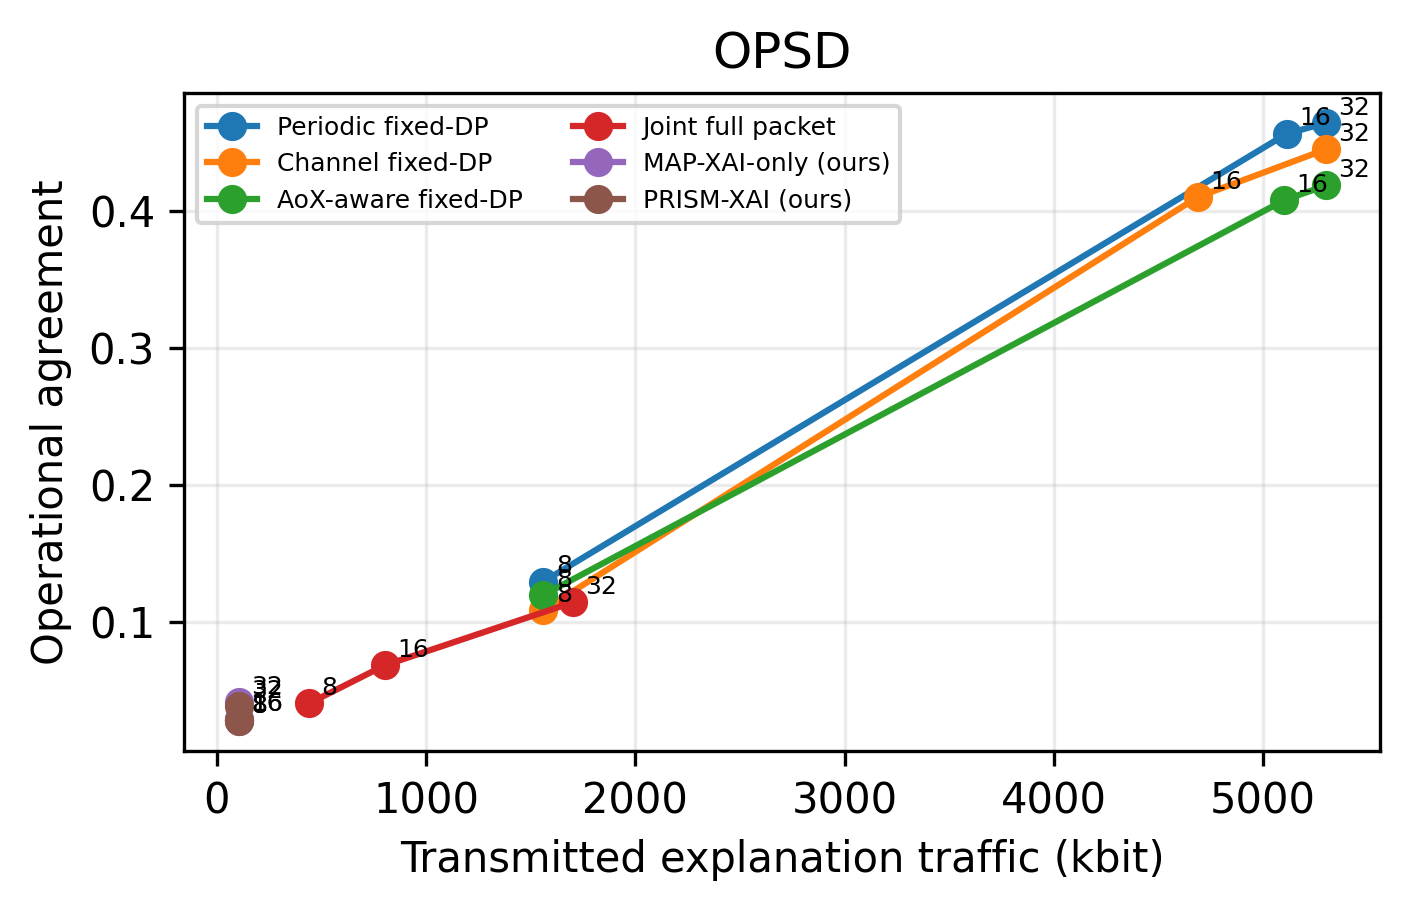
\includegraphics[width=\linewidth]{v19_pareto_opsd.png}\\[-1mm]{\small (a) Communication--operation}\end{minipage}\hfill
\begin{minipage}{.49\linewidth}\centering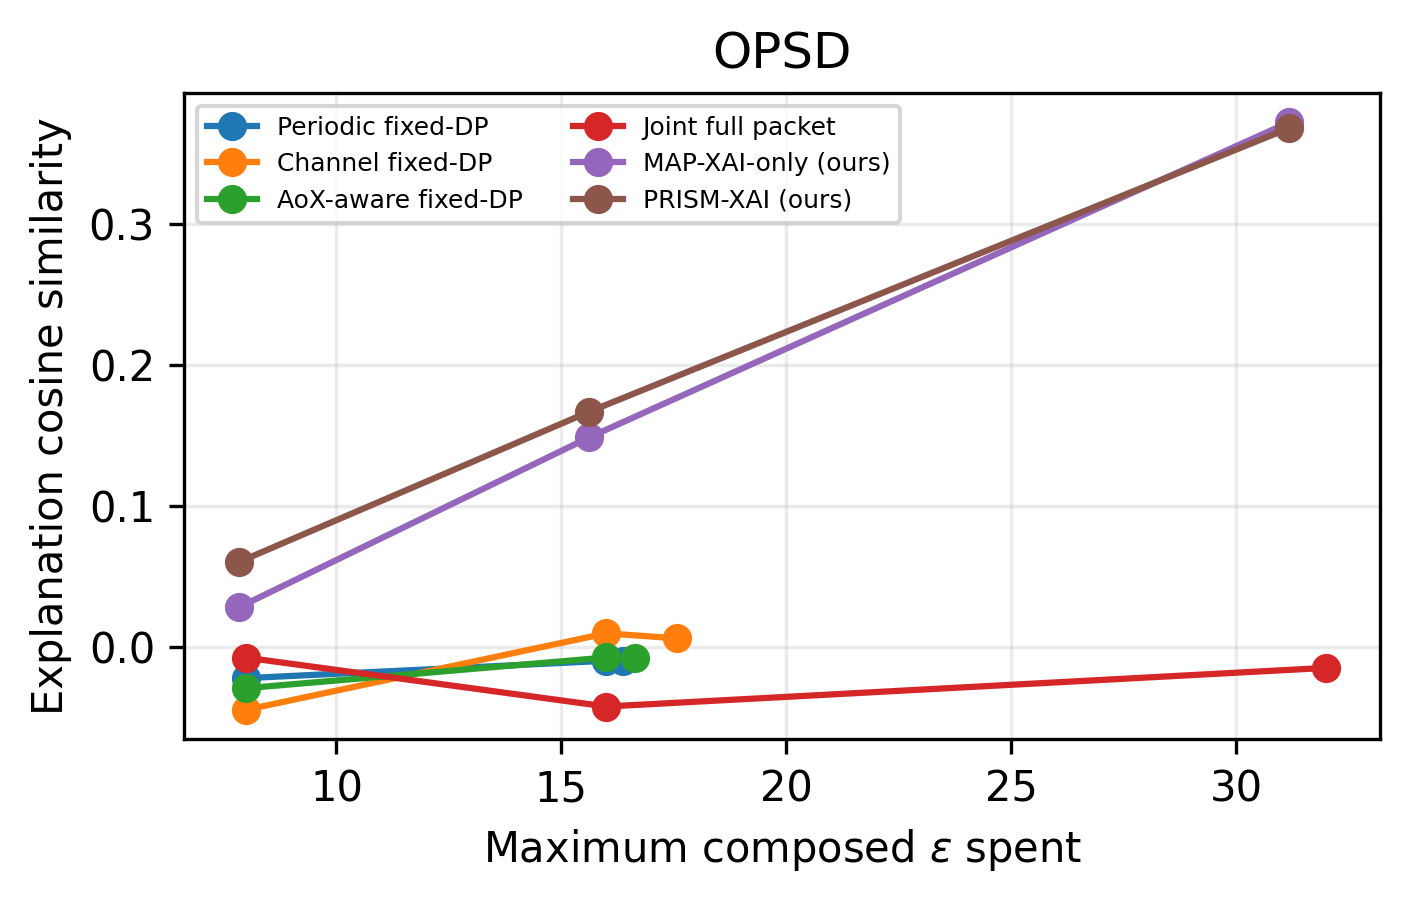
\includegraphics[width=\linewidth]{v19_privacy_fidelity_opsd.png}\\[-1mm]{\small (b) Privacy--fidelity}\end{minipage}
\caption{OPSD v19 M8 decomposed views. The proposed modes stay in the low-traffic region and show the clearest fidelity improvement as the privacy allowance increases.}
\label{fig:opsd-main}
\end{figure}

OPSD also illustrates why precision and recall must be separated. The proposed stack recalls fewer critical events because it covers fewer events, yet its accepted interventions are more precise and require fewer transmitted bits per correct decision. This is a selective decision-support regime, not an exhaustive alarm-service regime.


\subsection{UCI: operational selectivity survives even when attribution fidelity is weak}
On UCI, PRISM averages 379.4 kbit, critical coverage 0.086, recall 0.042, precision 0.640, and fairness 0.992. However, Top-$K$ is only 0.240 and cosine 0.012, close to the random/zero region. \MAP{}-only has Top-$K$ 0.229 and cosine 0.056. Thus UCI is the stronger counterexample to any claim that communication efficiency automatically implies high attribution reconstruction fidelity.

At the same time, intervention precision is much higher on UCI than OPSD. This difference is informative: operational precision and exact attribution similarity measure different properties. A scheduler may reject most opportunities and accept a small set of decisions that are operationally consistent even when the reconstructed private attribution vector is noisy. The result should therefore be presented as multi-metric evidence rather than collapsing fidelity and usefulness into a single number.


\begin{figure}[htbp]
\centering
\begin{minipage}{.49\linewidth}\centering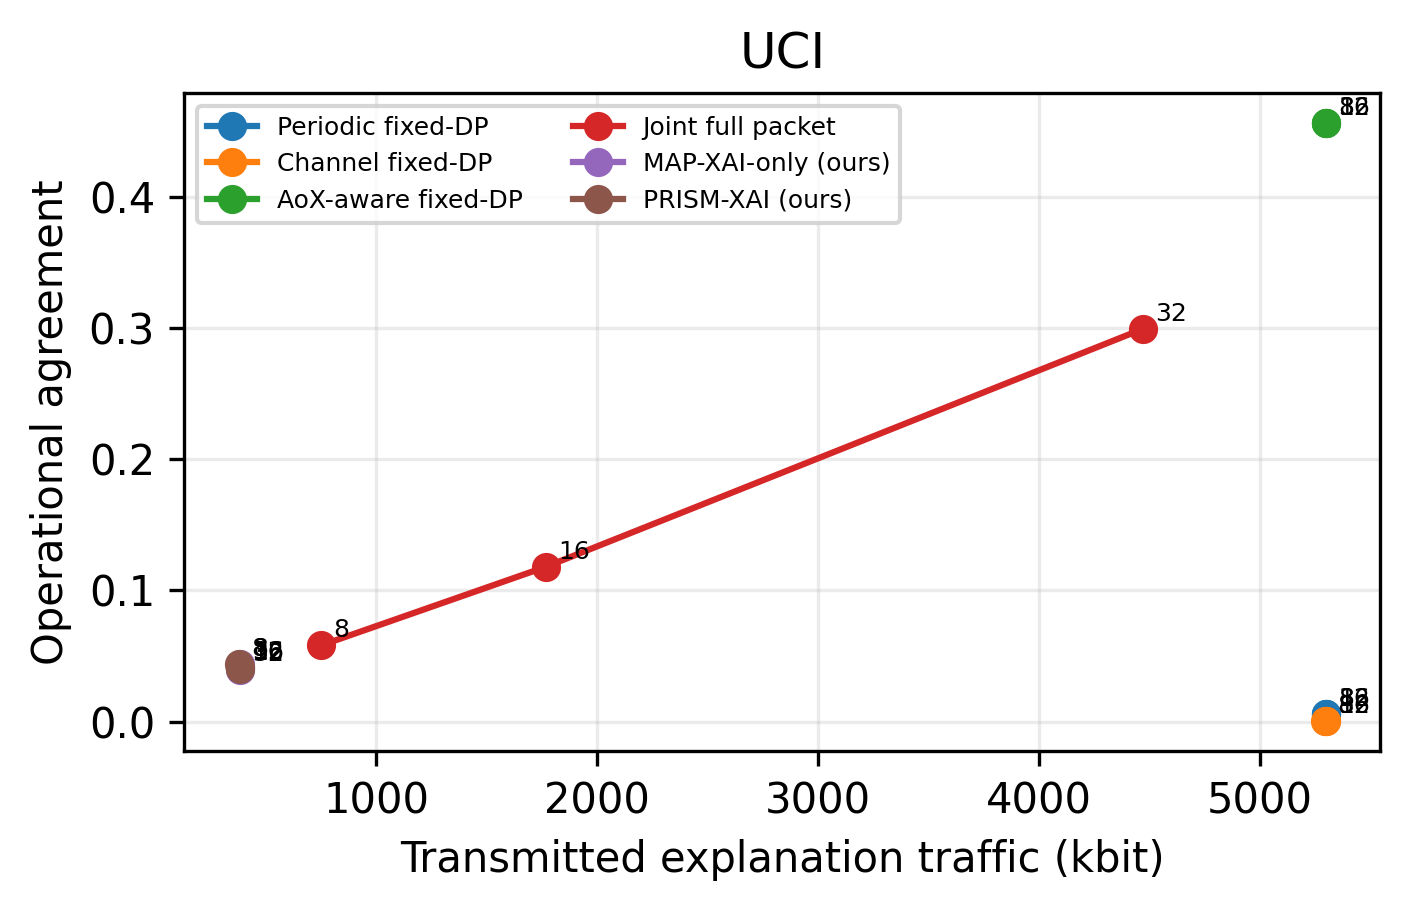
\includegraphics[width=\linewidth]{v19_pareto_uci.png}\\[-1mm]{\small (a) Communication--operation}\end{minipage}\hfill
\begin{minipage}{.49\linewidth}\centering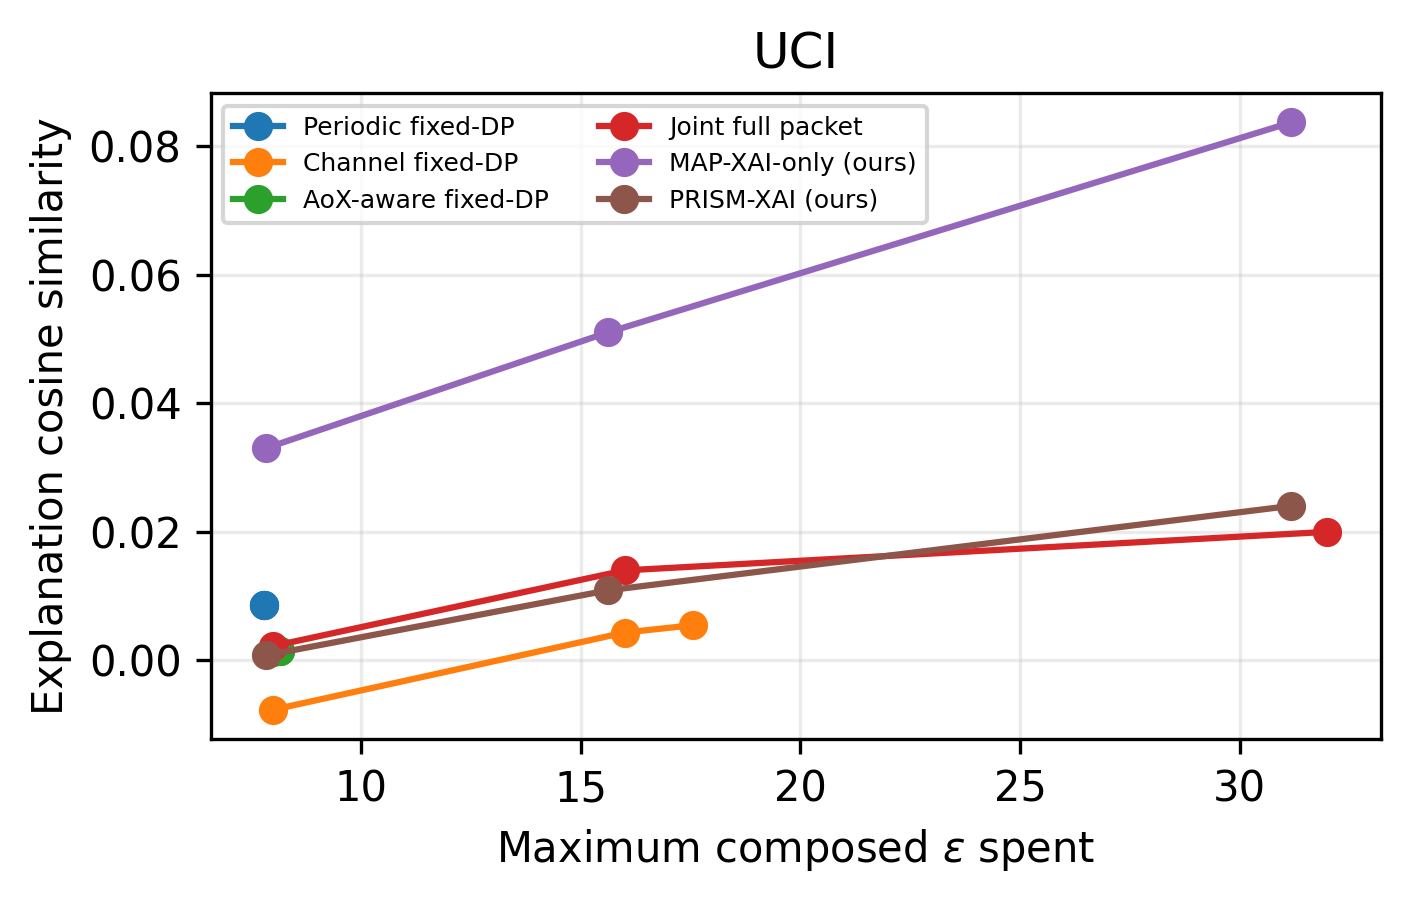
\includegraphics[width=\linewidth]{v19_privacy_fidelity_uci.png}\\[-1mm]{\small (b) Privacy--fidelity}\end{minipage}
\caption{UCI v19 M8 decomposed views. Communication savings remain strong, while explanation fidelity is much less responsive than on OPSD. This dataset is the clearest evidence that privacy/fidelity remains the limiting factor.}
\label{fig:uci-main}
\end{figure}

\subsection{Fairness--fidelity by dataset}
\begin{figure}[htbp]
\centering
\begin{minipage}{.49\linewidth}\centering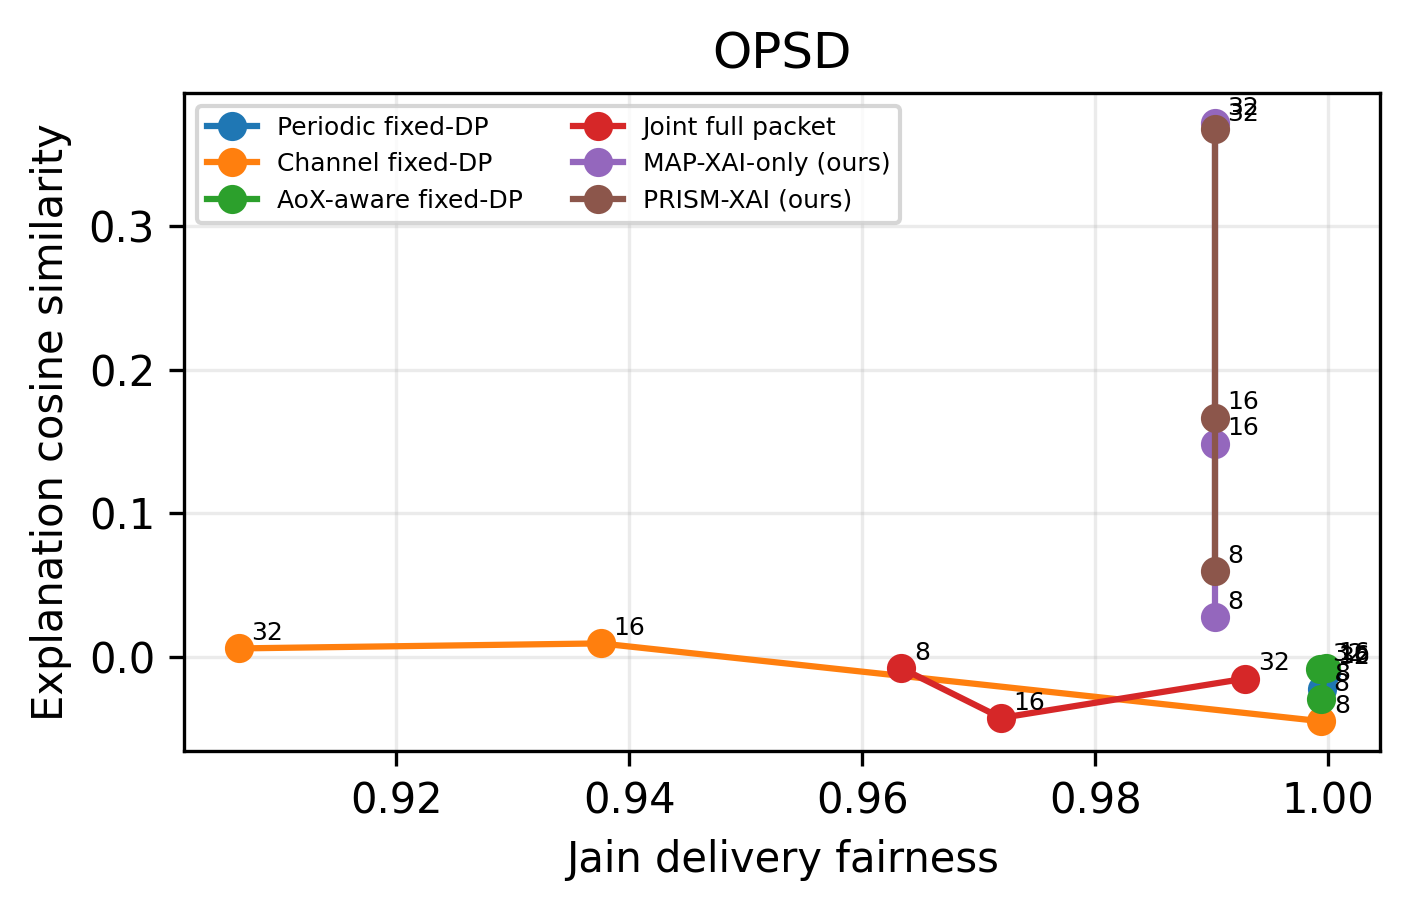
\includegraphics[width=\linewidth]{v19_fairness_fidelity_opsd.png}\\[-1mm]{\small (a) OPSD}\end{minipage}\hfill
\begin{minipage}{.49\linewidth}\centering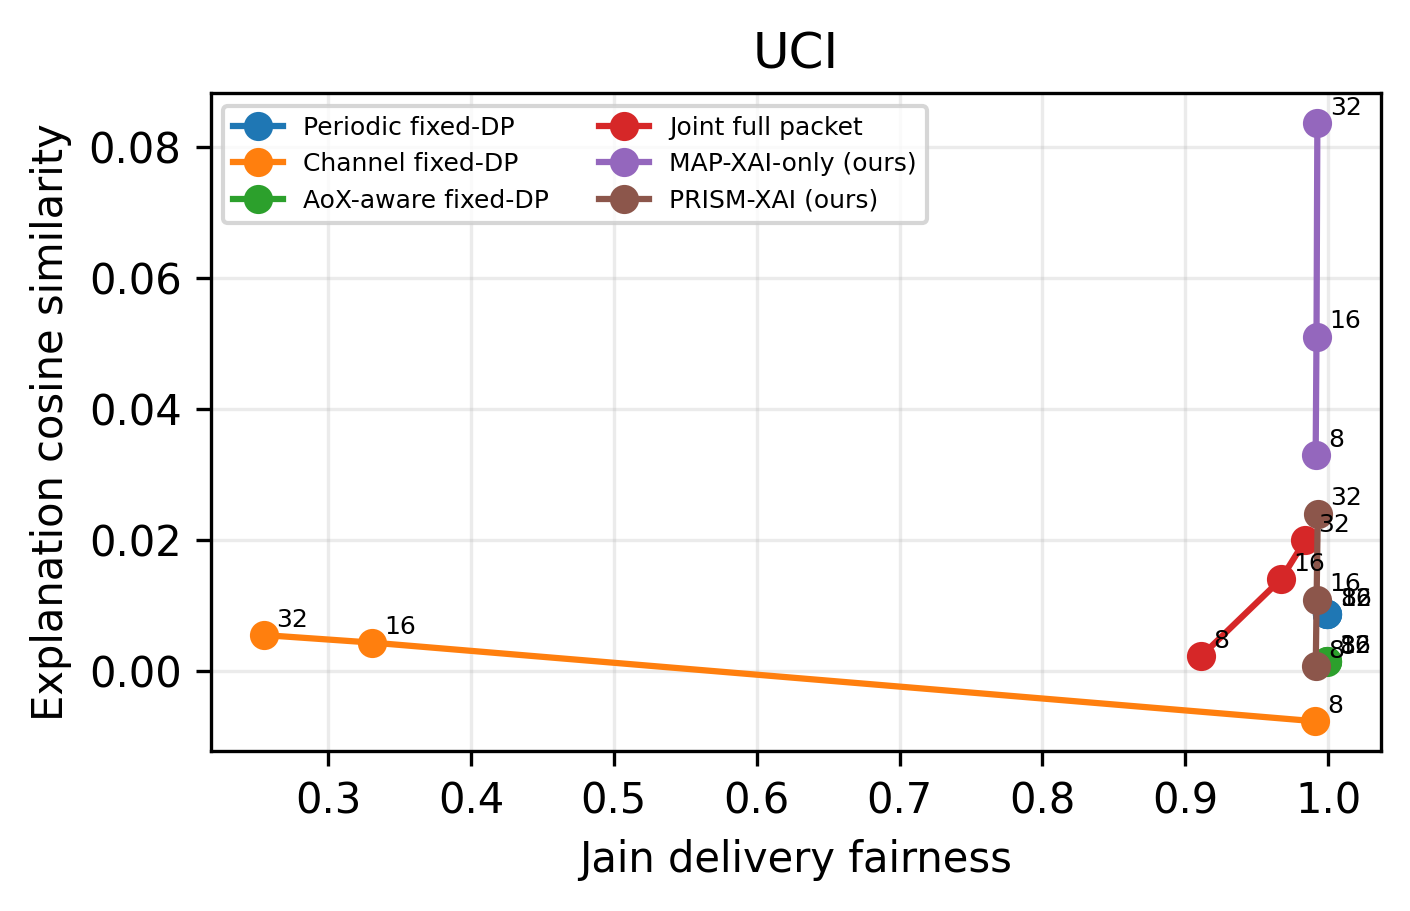
\includegraphics[width=\linewidth]{v19_fairness_fidelity_uci.png}\\[-1mm]{\small (b) UCI}\end{minipage}
\caption{Dataset-specific fairness--fidelity trade-off. PRISM/MAP-XAI-only remain in the high-fairness region on both datasets, whereas channel-aware fixed-DP can sacrifice fairness substantially on UCI.}
\label{fig:fair-datasets}
\end{figure}

\section{Privacy-budget sensitivity: what changes when \texorpdfstring{$\epsilon_{\max}$}{epsilon-max} increases?}
The M8 release cap is fixed while $\epsilon_{\max}$ changes from 8 to 16 to 32. This isolates the effect of assigning more privacy allowance to roughly the same number of private release opportunities. Table~\ref{tab:epsilon-scorecard} shows a clear pattern: PRISM traffic remains essentially constant at 240--244 kbit, while Top-$K$ improves from 0.232 to 0.253 to 0.351 and cosine from 0.030 to 0.089 to 0.196. Precision rises from 0.399 to 0.432 to 0.698. Coverage stays around 7--8\% and recall around 3.5--4.0\% because the release cap, not the privacy allowance, is the main service-frequency limiter in this experiment.

\begin{table}[htbp]\centering\small
\caption{Privacy-budget sensitivity of the proposed stack, averaged over both datasets, both XAI methods, and ten seeds. The M8 release cap is fixed across budgets.}
\label{tab:epsilon-scorecard}
\begin{tabular}{r l r r r r r r r r}
\toprule
$\epsilon_{\max}$ & Method & kbit & Top-K & Cos. & Crit. cov. & Recall & Prec. & bit/corr. & Jain \\
\midrule
8 & MAP-XAI-only (ours) & 243.8 & 0.227 & 0.030 & 0.081 & 0.036 & 0.396 & 10,421 & 0.991 \\
8 & PRISM-XAI (ours) & 240.4 & 0.232 & 0.030 & 0.081 & 0.036 & 0.399 & 10,193 & 0.991 \\
16 & MAP-XAI-only (ours) & 243.8 & 0.251 & 0.100 & 0.079 & 0.035 & 0.449 & 10,328 & 0.991 \\
16 & PRISM-XAI (ours) & 243.7 & 0.253 & 0.089 & 0.079 & 0.035 & 0.432 & 10,590 & 0.991 \\
32 & MAP-XAI-only (ours) & 243.6 & 0.318 & 0.228 & 0.074 & 0.041 & 0.770 & 9,132 & 0.991 \\
32 & PRISM-XAI (ours) & 243.5 & 0.351 & 0.196 & 0.075 & 0.040 & 0.698 & 9,179 & 0.991 \\
\bottomrule
\end{tabular}
\end{table}

This distinction is important. A larger privacy budget helps each selected packet carry a cleaner explanation, but it does not automatically make PRISM serve many more events when the M8 scheduler still permits only a small number of private releases. External baselines behave differently because they use the extra accounting headroom to transmit more frequently; for example, AoX fixed-DP coverage rises toward one. The privacy budget therefore controls both noise and, depending on the policy, the number of feasible releases.


\section{Attribution-method sensitivity}
The main conclusions are not produced by only one explanation algorithm. Under PRISM, TreeSHAP and feature ablation have almost identical traffic, coverage, recall, fairness, and bits per correct intervention. Feature ablation has somewhat higher macro Top-$K$ (0.286 versus 0.271) and cosine (0.118 versus 0.092), but the direction is not uniformly favorable inside \MAP{}-only, where feature ablation's cosine is especially high (0.149) while PRISM's is 0.118. This reinforces the intended internal relationship: full PRISM should not be forced to dominate \MAP{}-only on every reconstruction metric.

\begin{table}[htbp]\centering\small
\caption{XAI-method sensitivity for the proposed stack, averaged over both datasets, three privacy budgets, and ten seeds.}
\label{tab:xai-scorecard}
\begin{tabular}{llrrrrrrrr}
\toprule
XAI & Method & kbit & Top-K & Cos. & Crit. cov. & Recall & Prec. & bit/corr. & Jain \\
\midrule
TreeSHAP & MAP-XAI-only (ours) & 243.9 & 0.267 & 0.090 & 0.080 & 0.037 & 0.537 & 9,975 & 0.991 \\
TreeSHAP & PRISM-XAI (ours) & 243.2 & 0.271 & 0.092 & 0.080 & 0.037 & 0.509 & 9,885 & 0.991 \\
feature\_ablation & MAP-XAI-only (ours) & 243.5 & 0.264 & 0.148 & 0.076 & 0.038 & 0.539 & 9,945 & 0.991 \\
feature\_ablation & PRISM-XAI (ours) & 241.8 & 0.286 & 0.118 & 0.077 & 0.037 & 0.511 & 10,089 & 0.991 \\
\bottomrule
\end{tabular}
\end{table}

The forecasting table already showed identical RMSE/MAE across the two XAI choices. Hence this sensitivity analysis concerns explanation generation and scheduling rather than changes in predictive accuracy.


\section{MAP-XAI-only versus full PRISM: component relationship, not a baseline contest}
The paired outcomes are the cleanest evidence for how the two proposed layers relate. Across 12 dataset/XAI/privacy settings, PRISM and \MAP{}-only are statistically tied on critical-event recall, intervention coverage, deadline-miss rate, fairness, and bits per correct intervention in all 12 settings. PRISM traffic is significantly lower in five and tied in seven. Top-$K$ is higher once and tied 11 times. Cosine is mixed: PRISM is higher four times, tied twice, and lower six times. Intervention precision is tied ten times and lower twice.

This is exactly why \MAP{}-only should be treated as an internal restriction, not the ``strongest competing baseline.'' The full scheduler inherits the same protected packetization mechanism and broad service skeleton, then gains access to abstention, residual accumulation, alternative semantic modes, and gain-per-bit scheduling. In conditions where those extra actions are not useful, falling back toward \MAP{} behavior is desirable rather than a failure.

The small E--F feasibility diagnostic offers a concrete example. On OPSD, PRISM reduces traffic from 36.85 to 34.90 kbit and raises critical recall from 0.012 to 0.020 and precision from 0.249 to 0.466, but Top-$K$ falls from 0.284 to 0.246. On UCI, traffic falls from 115.8 to 114.0 kbit, recall rises from 0.008 to 0.009, precision from 0.269 to 0.291, and cosine from 0.023 to 0.030, while Top-$K$ falls from 0.260 to 0.222. The scheduler can therefore trade among operational and fidelity objectives; it is not expected to improve every one simultaneously.


\begin{table}[htbp]
\centering
\small
\caption{Scheduler stages E--F in the feasibility diagnostic (three seeds).}
\label{tab:ef}
\resizebox{\textwidth}{!}{%
\begin{tabular}{llrrrrrrrrrr}
\toprule
Data & Stage & kbit & Top-K & Cos. & Coverage & Recall & Prec. & False int. & Abstain & Jain & eps \\
\midrule
OPSD & E MAP-XAI-only & 36.85 & 0.284 & 0.003 & 0.034 & 0.012 & 0.249 & 0.010 & 0.966 & 0.988 & 3.703 \\
OPSD & F PRISM-XAI & 34.90 & 0.246 & 0.000 & 0.034 & 0.020 & 0.466 & 0.008 & 0.966 & 0.988 & 3.703 \\
UCI & E MAP-XAI-only & 115.8 & 0.260 & 0.023 & 0.018 & 0.008 & 0.269 & 0.017 & 0.982 & 0.943 & 3.703 \\
UCI & F PRISM-XAI & 114.0 & 0.222 & 0.030 & 0.018 & 0.009 & 0.291 & 0.016 & 0.982 & 0.943 & 3.703 \\
\bottomrule
\end{tabular}}
\end{table}


\section{External Reference Policies and Their Trade-offs}
The four external references answer different questions, so averaging them into one ``baseline'' category would obscure the result.

\paragraph{Periodic fixed-DP.} This policy is highly fair (Jain approximately 1.0) but extremely communication intensive. PRISM has lower traffic, energy, and bits per correct intervention in all 12 paired conditions. Precision is higher in 11 and tied in one. Recall is mixed because periodic service can cover more events, especially on conditions where its privacy/accounting configuration remains feasible.

\paragraph{Channel fixed-DP.} This baseline exposes the cost of scheduling only when the channel is attractive. Traffic remains extremely high, yet endpoint fairness drops sharply, especially on UCI. PRISM is significantly fairer in eight paired settings, tied in two, and worse in two, while still being lower in traffic/energy/bits-per-correct in all 12. Recall is split because the channel policy nearly collapses coverage in some UCI conditions but can serve more on OPSD.

\paragraph{AoX fixed-DP.} AoX scheduling is the strongest service-frequency reference. It achieves the highest macro coverage and recall and near-perfect fairness, and therefore PRISM loses recall and fairness in all 12 paired comparisons. But it pays for this with substantially larger traffic and energy. PRISM wins traffic and energy in all 12, bits per correct in 10 with two ties, cosine in seven with five ties, and precision in 11 with one tie. This baseline makes the central trade-off explicit rather than threatening the contribution: exhaustive freshness and high recall are possible if the system is willing to transmit much more.

\paragraph{Joint full packet.} This reference asks what happens when compression/selectivity are relaxed. It improves coverage/recall relative to PRISM but still consumes far more traffic and energy. PRISM has lower traffic and energy in all 12 settings and lower bits per correct intervention in 11 with one tie. Precision is higher in eight and tied in four. Top-$K$ is mostly tied, showing that simply sending a larger private packet does not reliably recover the explanation once DP noise dominates.

\section{Paired Statistical Evidence Across Matched Conditions}

The macro-average results summarize the dominant behavior of the evaluated schedulers, but averages alone do not establish whether an apparent advantage is repeated consistently across experimental conditions. A large mean improvement can, in principle, be produced by a small number of unusually favorable dataset, XAI, or privacy configurations. The paired statistical analysis therefore evaluates PRISM-XAI against each reference under matched experimental conditions.

For every fixed dataset, XAI method, privacy budget, and random seed, the PRISM-XAI result is paired with the corresponding reference-policy result generated under the same stochastic realization. The resulting seed-wise differences are used to construct 95\% confidence intervals. A comparison is classified as favorable only when the complete confidence interval lies on the favorable side of zero; it is classified as unfavorable when the complete interval lies on the opposite side; and it is treated as a tie when the interval contains zero.

This procedure provides a stricter test than comparing macro means because an apparent difference must repeat across paired stochastic realizations rather than arise from unrelated run variability.


\setlength{\tabcolsep}{3pt}
\renewcommand{\arraystretch}{1.08}
\begin{longtable}{llrrrr}
\caption{Sign-of-95\% CI outcome counts for PRISM versus each reference and metric.}\label{tab:paircounts}\\
\toprule
Reference & Metric & n & PRISM better & Tie & PRISM worse \\
\midrule
\endfirsthead
\toprule
Reference & Metric & n & PRISM better & Tie & PRISM worse \\
\midrule
\endhead
\midrule
\multicolumn{6}{r}{Continued on next page} \\
\endfoot
\bottomrule
\endlastfoot
AoX-aware fixed-DP & transmitted\_kbits & 12 & 12 & 0 & 0 \\
AoX-aware fixed-DP & bits\_per\_correct\_intervention & 12 & 10 & 2 & 0 \\
AoX-aware fixed-DP & energy\_mj & 12 & 12 & 0 & 0 \\
AoX-aware fixed-DP & deadline\_miss\_rate & 12 & 1 & 11 & 0 \\
AoX-aware fixed-DP & topk\_overlap & 12 & 2 & 9 & 1 \\
AoX-aware fixed-DP & cosine\_similarity & 12 & 7 & 5 & 0 \\
AoX-aware fixed-DP & critical\_event\_recall & 12 & 0 & 0 & 12 \\
AoX-aware fixed-DP & intervention\_precision & 12 & 11 & 1 & 0 \\
AoX-aware fixed-DP & intervention\_coverage & 12 & 0 & 0 & 12 \\
AoX-aware fixed-DP & jain\_delivery\_fairness & 12 & 0 & 0 & 12 \\
Channel fixed-DP & transmitted\_kbits & 12 & 12 & 0 & 0 \\
Channel fixed-DP & bits\_per\_correct\_intervention & 12 & 12 & 0 & 0 \\
Channel fixed-DP & energy\_mj & 12 & 12 & 0 & 0 \\
Channel fixed-DP & deadline\_miss\_rate & 12 & 0 & 12 & 0 \\
Channel fixed-DP & topk\_overlap & 12 & 2 & 10 & 0 \\
Channel fixed-DP & cosine\_similarity & 12 & 7 & 5 & 0 \\
Channel fixed-DP & critical\_event\_recall & 12 & 6 & 0 & 6 \\
Channel fixed-DP & intervention\_precision & 12 & 8 & 4 & 0 \\
Channel fixed-DP & intervention\_coverage & 12 & 6 & 0 & 6 \\
Channel fixed-DP & jain\_delivery\_fairness & 12 & 8 & 2 & 2 \\
Joint full packet & transmitted\_kbits & 12 & 12 & 0 & 0 \\
Joint full packet & bits\_per\_correct\_intervention & 12 & 11 & 1 & 0 \\
Joint full packet & energy\_mj & 12 & 12 & 0 & 0 \\
Joint full packet & deadline\_miss\_rate & 12 & 0 & 12 & 0 \\
Joint full packet & topk\_overlap & 12 & 2 & 9 & 1 \\
Joint full packet & cosine\_similarity & 12 & 4 & 8 & 0 \\
Joint full packet & critical\_event\_recall & 12 & 0 & 2 & 10 \\
Joint full packet & intervention\_precision & 12 & 8 & 4 & 0 \\
Joint full packet & intervention\_coverage & 12 & 0 & 0 & 12 \\
Joint full packet & jain\_delivery\_fairness & 12 & 10 & 2 & 0 \\
Periodic fixed-DP & transmitted\_kbits & 12 & 12 & 0 & 0 \\
Periodic fixed-DP & bits\_per\_correct\_intervention & 12 & 12 & 0 & 0 \\
Periodic fixed-DP & energy\_mj & 12 & 12 & 0 & 0 \\
Periodic fixed-DP & deadline\_miss\_rate & 12 & 0 & 12 & 0 \\
Periodic fixed-DP & topk\_overlap & 12 & 2 & 9 & 1 \\
Periodic fixed-DP & cosine\_similarity & 12 & 7 & 5 & 0 \\
Periodic fixed-DP & critical\_event\_recall & 12 & 6 & 0 & 6 \\
Periodic fixed-DP & intervention\_precision & 12 & 11 & 1 & 0 \\
Periodic fixed-DP & intervention\_coverage & 12 & 6 & 0 & 6 \\
Periodic fixed-DP & jain\_delivery\_fairness & 12 & 0 & 0 & 12 \\
MAP-XAI-only (ours) & transmitted\_kbits & 12 & 5 & 7 & 0 \\
MAP-XAI-only (ours) & bits\_per\_correct\_intervention & 12 & 0 & 12 & 0 \\
MAP-XAI-only (ours) & energy\_mj & 12 & 4 & 8 & 0 \\
MAP-XAI-only (ours) & deadline\_miss\_rate & 12 & 0 & 12 & 0 \\
MAP-XAI-only (ours) & topk\_overlap & 12 & 1 & 11 & 0 \\
MAP-XAI-only (ours) & cosine\_similarity & 12 & 4 & 2 & 6 \\
MAP-XAI-only (ours) & critical\_event\_recall & 12 & 0 & 12 & 0 \\
MAP-XAI-only (ours) & intervention\_precision & 12 & 0 & 10 & 2 \\
MAP-XAI-only (ours) & intervention\_coverage & 12 & 0 & 12 & 0 \\
MAP-XAI-only (ours) & jain\_delivery\_fairness & 12 & 0 & 12 & 0 \\
\end{longtable}

The outcome counts show that the strongest repeated advantages of PRISM-XAI are associated with communication and energy efficiency. Transmitted traffic is lower than all four external references in every matched comparison, yielding 48 favorable outcomes out of 48 external-reference conditions. The same communication reduction is reflected in the energy metric because the modeled transmission energy scales with the amount of communicated data.

Bits per correct intervention show a similarly strong pattern. PRISM-XAI is favorable in 45 of the 48 external comparisons and tied in the remaining three. This result indicates that, despite serving fewer critical events overall, the proposed scheduler usually requires substantially less communication for each correct critical intervention that it produces.

Intervention precision is also highly consistent. PRISM-XAI is favorable in 38 of 48 external comparisons and tied in the remaining ten, with no unfavorable external condition. This pattern is consistent with selective explanation delivery: the scheduler transmits for fewer events, but the accepted critical interventions are concentrated more strongly on useful cases.

Exact attribution identity, measured through Top-$K$ agreement, is substantially less uniform. Across the 48 external comparisons, only eight conditions favor PRISM-XAI, 37 are statistically tied, and three are unfavorable. The Top-$K$ result therefore does not support a claim of universal attribution-fidelity dominance. Instead, it shows that PRISM-XAI usually preserves a level of dominant-feature agreement statistically comparable to the reference policies while operating at much lower traffic.

Critical-event recall exhibits the opposite structural behavior. PRISM-XAI is intentionally more selective than high-frequency policies such as AoX fixed-DP and therefore does not dominate recall. The unfavorable recall comparisons are consistent with the lower service frequency observed throughout the M8 evaluation rather than with a hidden inconsistency in the macro averages.

The paired counts therefore reinforce the interpretation of PRISM-XAI as a selective operating point. Communication efficiency, energy efficiency, bits per correct intervention, and intervention precision are the most statistically repeatable advantages. Exact Top-$K$ fidelity is predominantly comparable rather than superior, while critical-event recall is often lower because the scheduler intentionally serves fewer events.

The complete 60 paired comparisons are reported in Appendix~\ref{app:paired}, including every favorable, tied, and unfavorable condition. This allows the aggregate outcome counts to be traced directly to the corresponding dataset, XAI method, privacy budget, and reference policy.

\section{Temporal Regime Analysis}

The aggregate communication, Age-of-Explanation, privacy, and service metrics do not show when private releases are consumed during the evaluation horizon. The representative v19 M8 trace in Fig.~\ref{fig:orig-regime} provides that temporal context, while the decomposed traces below isolate explanation similarity, AoX, remaining privacy, and the critical-zone process.

\begin{figure}[htbp]
\centering
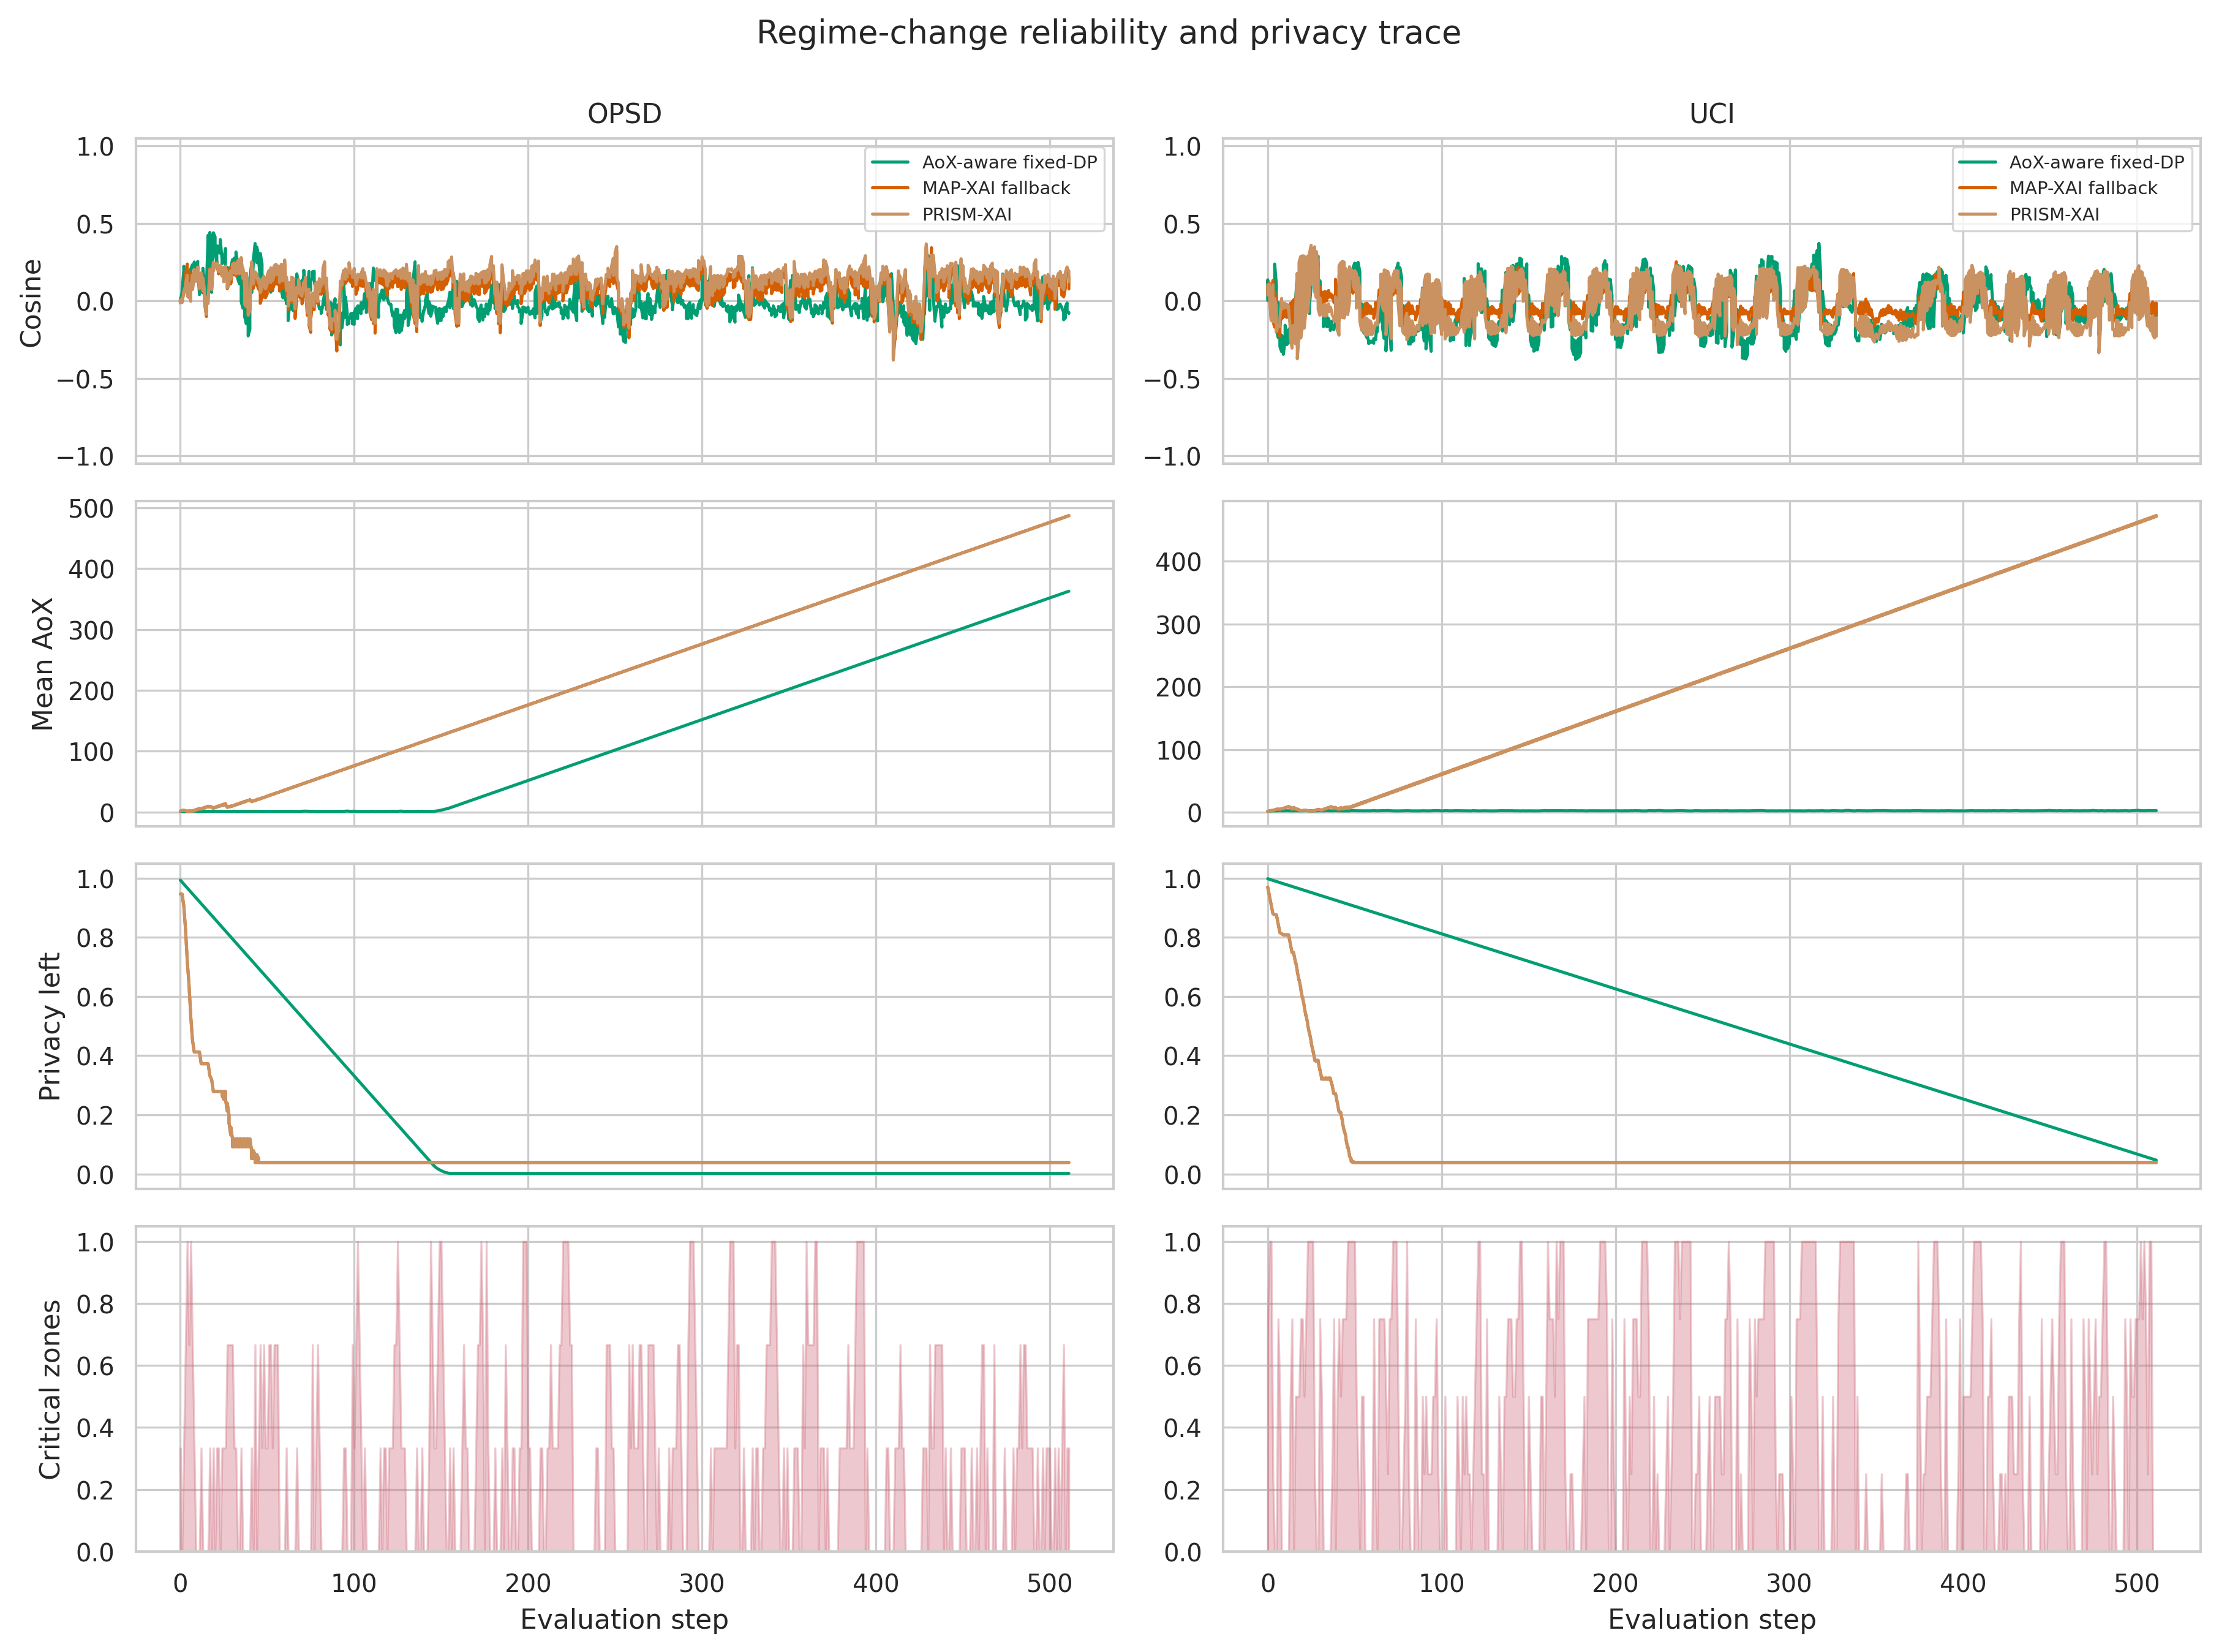
\includegraphics[width=.97\linewidth]{original_v19_M8_regime_trace.png}
\caption{Original v19 M8 representative regime trace. The selective MAP-XAI-only and PRISM-XAI configurations stop frequent private transmission after their finite release opportunities are largely consumed, whereas AoX fixed-DP continues refreshing explanations throughout the horizon.}
\label{fig:orig-regime}
\end{figure}

\subsection{Temporal Explanation Similarity}

\begin{figure}[htbp]
\centering
\begin{minipage}{.49\linewidth}
\centering
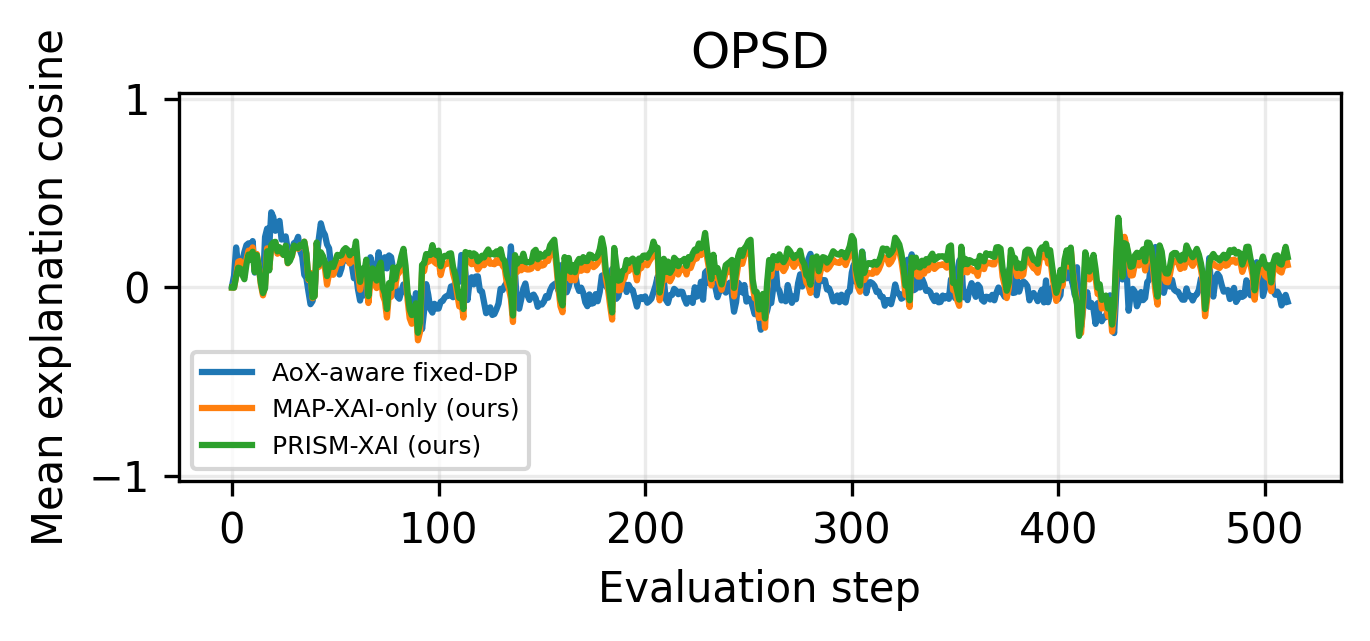
\includegraphics[width=\linewidth]{regime_cosine_opsd.png}\\[-1mm]
{\small (a) OPSD explanation cosine}
\end{minipage}\hfill
\begin{minipage}{.49\linewidth}
\centering
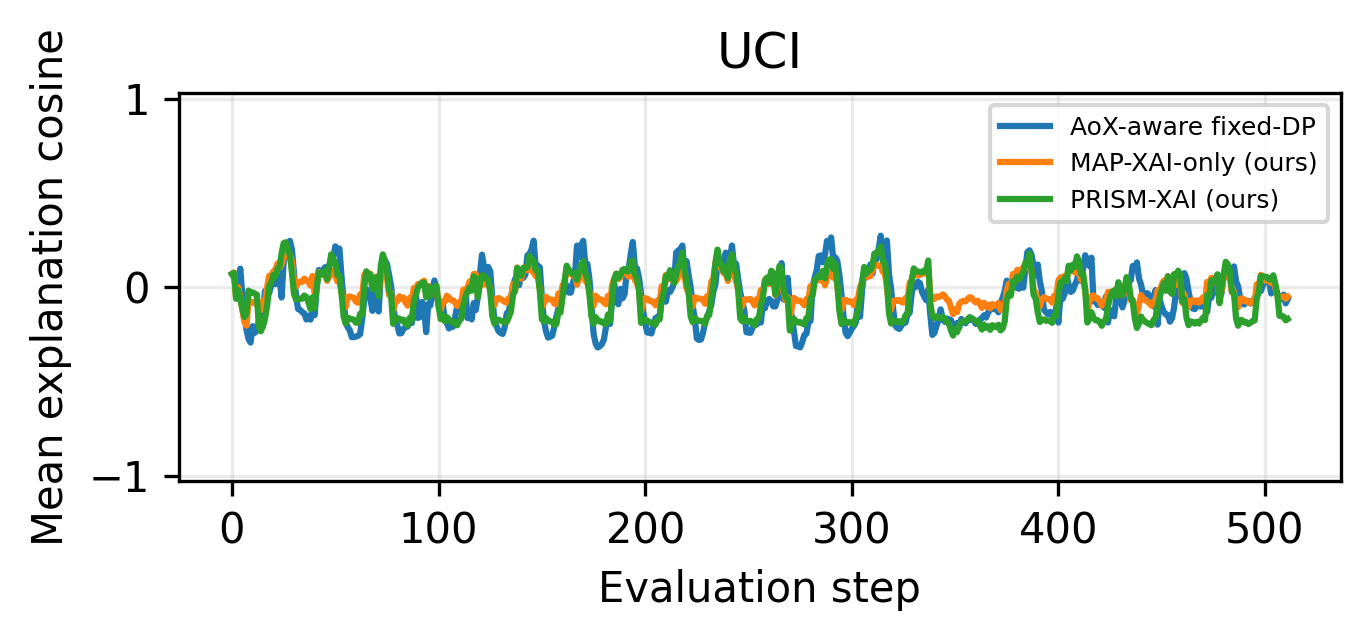
\includegraphics[width=\linewidth]{regime_cosine_uci.png}\\[-1mm]
{\small (b) UCI explanation cosine}
\end{minipage}
\caption{Temporal explanation similarity for the representative v19 M8 trace. OPSD retains more positive attribution structure than UCI, consistent with the dataset-dependent fidelity behavior observed in the aggregate results.}
\label{fig:regime_cosine}
\end{figure}

The decomposed cosine traces in Fig.~\ref{fig:regime_cosine} show that the dataset-level differences observed in the aggregate fidelity metrics persist temporally. OPSD generally retains more positive explanation similarity under the proposed modes, whereas UCI remains close to zero and exhibits substantially noisier behavior.

This pattern is consistent with the condition-level and feasibility-ladder analyses. The scheduler is not creating the UCI fidelity collapse at isolated time steps; rather, the private explanations entering the scheduling process already contain weak attribution structure. The temporal trace therefore reinforces the conclusion that the principal fidelity limitation originates in the privacy mechanism and dataset interaction.

\subsection{Temporal Age of Explanation}

\begin{figure}[htbp]
\centering
\begin{minipage}{.49\linewidth}
\centering
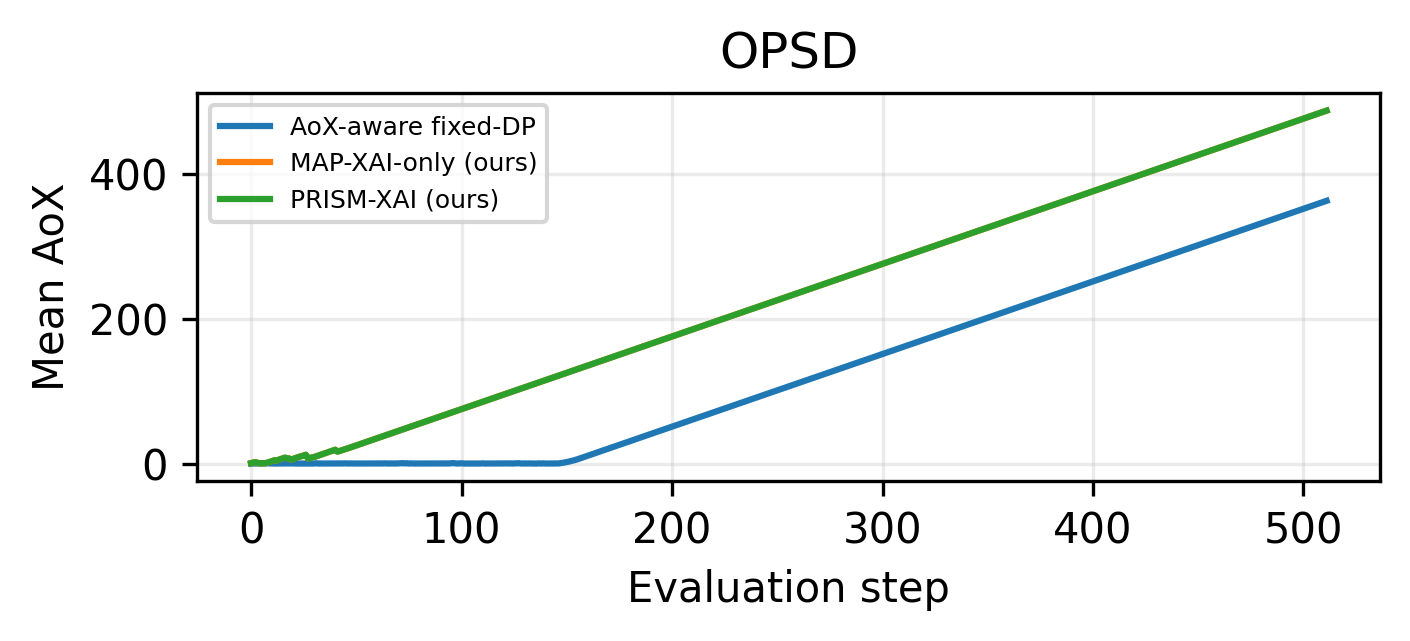
\includegraphics[width=\linewidth]{regime_aox_opsd.png}\\[-1mm]
{\small (a) OPSD mean AoX}
\end{minipage}\hfill
\begin{minipage}{.49\linewidth}
\centering
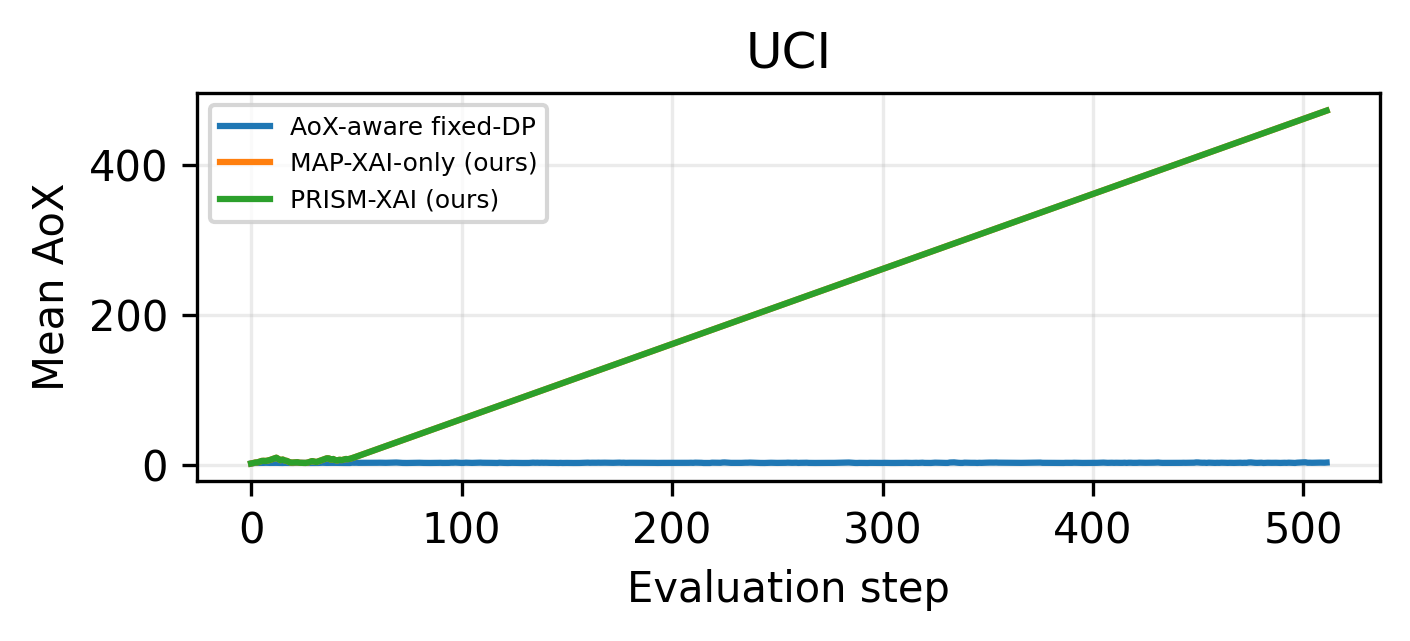
\includegraphics[width=\linewidth]{regime_aox_uci.png}\\[-1mm]
{\small (b) UCI mean AoX}
\end{minipage}
\caption{Temporal Age of Explanation. AoX increases under selective modes after private-release opportunities become sparse, while AoX fixed-DP continues refreshing explanations at substantially higher communication cost.}
\label{fig:regime_aox}
\end{figure}

Figure~\ref{fig:regime_aox} provides the temporal explanation for the large macro AoX difference. During the initial part of the horizon, MAP-XAI-only and PRISM-XAI transmit selected explanation updates and keep AoX comparatively controlled. As the finite release allowance is consumed, fewer new explanations are delivered and AoX begins to increase.

AoX fixed-DP behaves differently because freshness is its primary scheduling objective. It continues to transmit throughout the horizon and therefore maintains a much smaller AoX. This freshness advantage is achieved with substantially greater traffic and energy expenditure, as reported in the macro network metrics.

The AoX comparison should therefore be interpreted as a service-policy trade-off rather than as evidence that selective scheduling improves freshness. PRISM-XAI explicitly sacrifices continuous explanation freshness in order to preserve communication and privacy resources.

\subsection{Temporal Privacy Expenditure}

\begin{figure}[htbp]
\centering
\begin{minipage}{.49\linewidth}
\centering
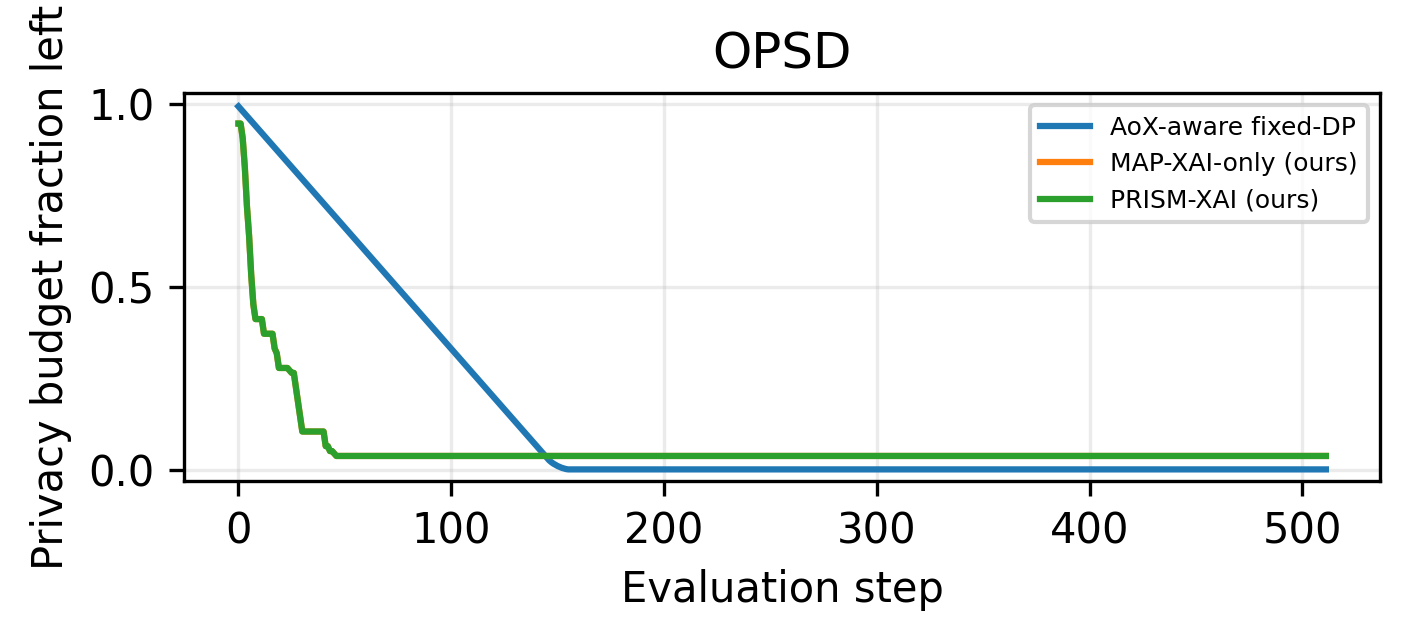
\includegraphics[width=\linewidth]{regime_privacy_opsd.png}\\[-1mm]
{\small (a) OPSD remaining privacy}
\end{minipage}\hfill
\begin{minipage}{.49\linewidth}
\centering
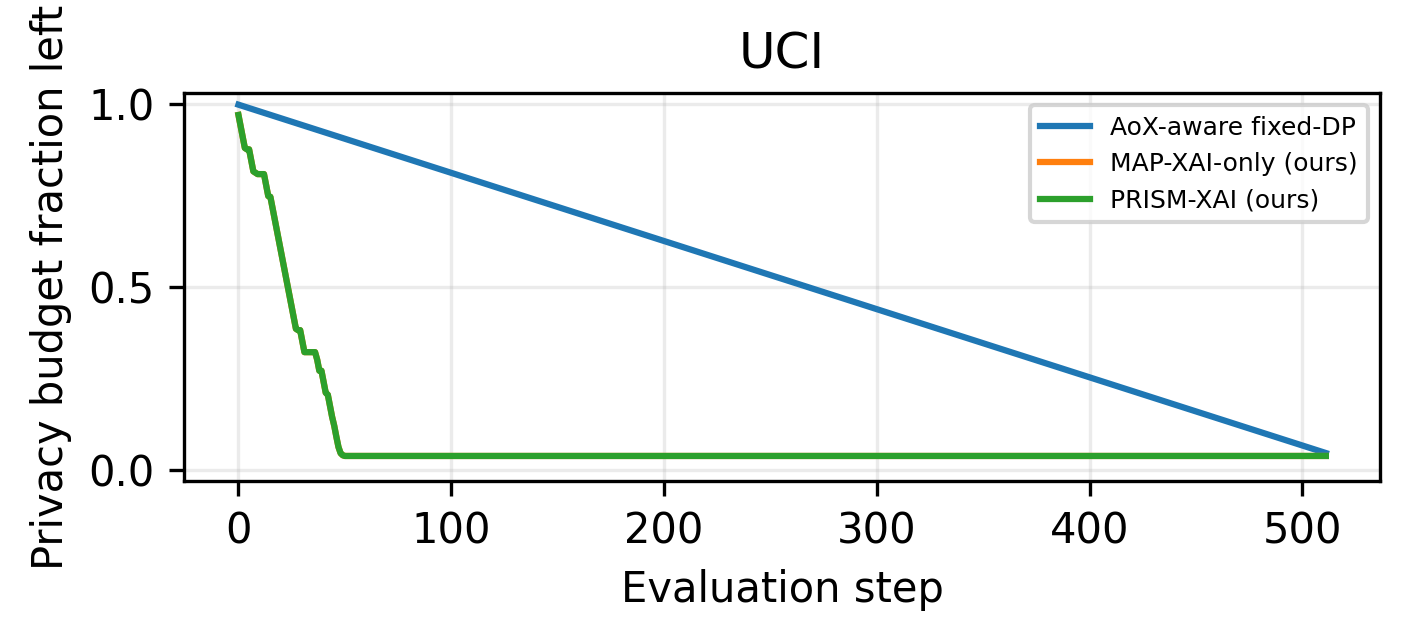
\includegraphics[width=\linewidth]{regime_privacy_uci.png}\\[-1mm]
{\small (b) UCI remaining privacy}
\end{minipage}
\caption{Remaining privacy over the representative v19 M8 trace. MAP-XAI-only and PRISM-XAI explicitly consume a finite household-level privacy allowance rather than treating successive releases as independently private.}
\label{fig:regime_privacy}
\end{figure}

The remaining-privacy traces in Fig.~\ref{fig:regime_privacy} show the cumulative nature of the household-level privacy constraint. Each private explanation release consumes part of the finite horizon-level allowance. The available privacy resource therefore decreases as the scheduler selects private transmissions.

This behavior is essential to the proposed formulation. The privacy budget is not reset for each packet, and the scheduler cannot continue releasing explanations indefinitely while claiming the same horizon-level privacy guarantee. Once much of the release allowance has been used, later explanation updates become constrained even when potentially important operating conditions occur.

The trace also shows why the temporal placement of releases matters. Two schedulers can use the same total number of private releases but obtain different operational outcomes if one consumes them early and another reserves a portion of the budget for later critical periods.

\subsection{Temporal Distribution of Critical Events}

\begin{figure}[htbp]
\centering
\begin{minipage}{.49\linewidth}
\centering
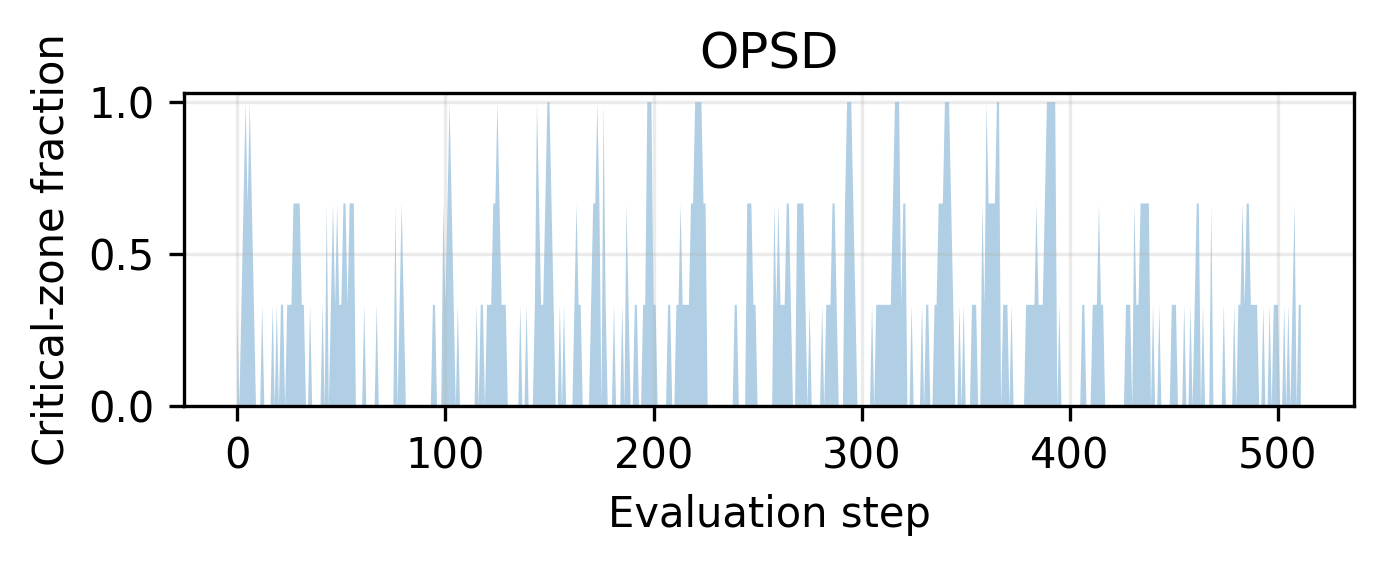
\includegraphics[width=\linewidth]{regime_critical_opsd.png}\\[-1mm]
{\small (a) OPSD critical-zone process}
\end{minipage}\hfill
\begin{minipage}{.49\linewidth}
\centering
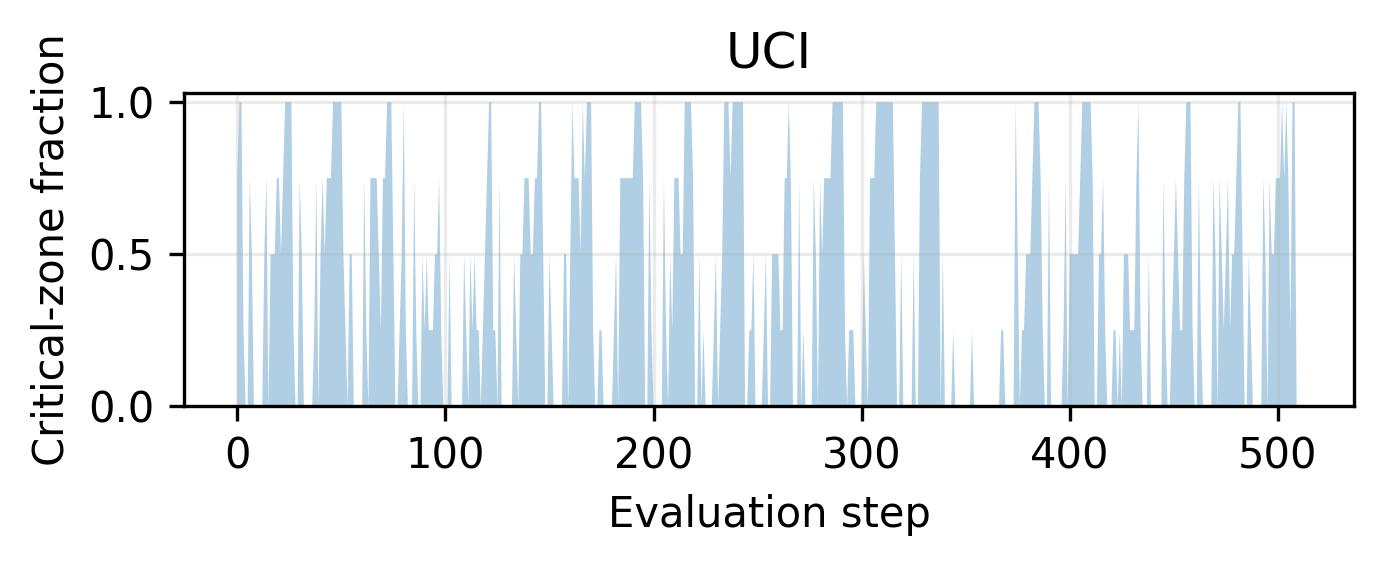
\includegraphics[width=\linewidth]{regime_critical_uci.png}\\[-1mm]
{\small (b) UCI critical-zone process}
\end{minipage}
\caption{Public critical-zone process during the representative evaluation horizon. Critical events continue to occur after substantial portions of the selective private-release allowance have already been consumed.}
\label{fig:regime_critical}
\end{figure}

Figure~\ref{fig:regime_critical} completes the temporal explanation of the recall and coverage results. Critical operating periods are distributed throughout the evaluation horizon rather than concentrated only at the beginning. Consequently, some critical events occur after MAP-XAI-only and PRISM-XAI have already consumed a substantial fraction of their finite private-release opportunities.

This temporal mismatch explains why the M8 selective modes cannot reproduce the recall of AoX fixed-DP under the same release policy. The issue is not solely the total number of private releases; it is also their allocation over time. Spending the available release opportunities too early leaves later critical events without fresh private explanations.

The temporal evidence therefore motivates two possible extensions of the current design. The scheduler could explicitly reserve part of the remaining privacy allowance for future high-criticality periods, or the privacy horizon could be shortened so that privacy resources are refreshed over smaller operational windows. Both approaches would alter the service--privacy trade-off and therefore require separate evaluation.

Overall, the temporal traces connect the aggregate metrics to the actual scheduling process. The large AoX values arise after selective transmission becomes sparse, the finite privacy allowance is progressively consumed, and critical events continue to occur throughout the horizon. The resulting lower late-horizon coverage is therefore a direct consequence of the current release-allocation policy.

\part{Mechanism Studies: Explaining the Observed Trade-offs}

\section{M8 versus M4 Release-Cap Sensitivity}

The M8 main configuration allows at most eight private releases per endpoint over the evaluation horizon. The M4 sensitivity study reduces this limit to four in order to test whether a more aggressive selective policy can further improve communication efficiency without violating the declared operational service requirement.

Reducing the release cap produces the expected communication benefit. Mean PRISM-XAI traffic falls from \(242.5\) kbit under M8 to \(120.5\) kbit under M4, corresponding to approximately a further halving of the already selective communication load.

The smaller release cap also improves several metrics computed over the accepted transmissions. Mean Top-$K$ agreement increases from \(0.279\) to \(0.310\), while intervention precision increases from \(0.510\) to \(0.712\). These values show that a highly restrictive release policy can concentrate the limited transmitted explanations on a smaller subset of comparatively favorable opportunities.

However, the same restriction substantially reduces explanation service. Mean critical-event coverage decreases from \(7.82\%\) under M8 to \(4.24\%\) under M4. More importantly, 100 of the 120 M4 PRISM-XAI runs fall below the configured \(5\%\) critical-event coverage floor. In contrast, every M8 PRISM-XAI run remains above the same threshold, with the minimum observed M8 coverage equal to approximately \(5.98\%\).


Fairness remains high on average in both configurations, but its worst-case behavior also deteriorates under the tighter release cap. Minimum Jain fairness decreases from approximately \(0.972\) under M8 to approximately \(0.933\) under M4. The result indicates that extreme selectivity can also increase variability in how the limited release opportunities are distributed across endpoints.


\scriptsize
\setlength{\tabcolsep}{3pt}
\renewcommand{\arraystretch}{1.08}
\begin{longtable}{lrrrrrrrrrrrr}
\caption{v19 selective-release-cap sensitivity. M8 is used in the main paper because it satisfies the 5\% critical-coverage guardrail in every PRISM run.}\label{tab:m4m8}\\
\toprule
Cap & n & kbit & Mean cov. & Min cov. & Recall & Prec. & Top-K & Cos. & Jain & bit/corr. & Runs cov.<5\% & Priv. viol. \\
\midrule
\endfirsthead
\toprule
Cap & n & kbit & Mean cov. & Min cov. & Recall & Prec. & Top-K & Cos. & Jain & bit/corr. & Runs cov.<5\% & Priv. viol. \\
\midrule
\endhead
\midrule
\multicolumn{13}{r}{Continued on next page} \\
\endfoot
\bottomrule
\endlastfoot
M4 & 120 & 120.5 & 0.042 & 0.030 & 0.022 & 0.712 & 0.310 & 0.116 & 0.984 & 8,810.0 & 100 & 0 \\
M8 & 120 & 242.5 & 0.078 & 0.060 & 0.037 & 0.510 & 0.279 & 0.105 & 0.991 & 9,987.0 & 0 & 0 \\
\end{longtable}


\subsection{Communication and Fidelity under M4}

\begin{figure}[htbp]
\centering
\begin{minipage}{.49\linewidth}
\centering
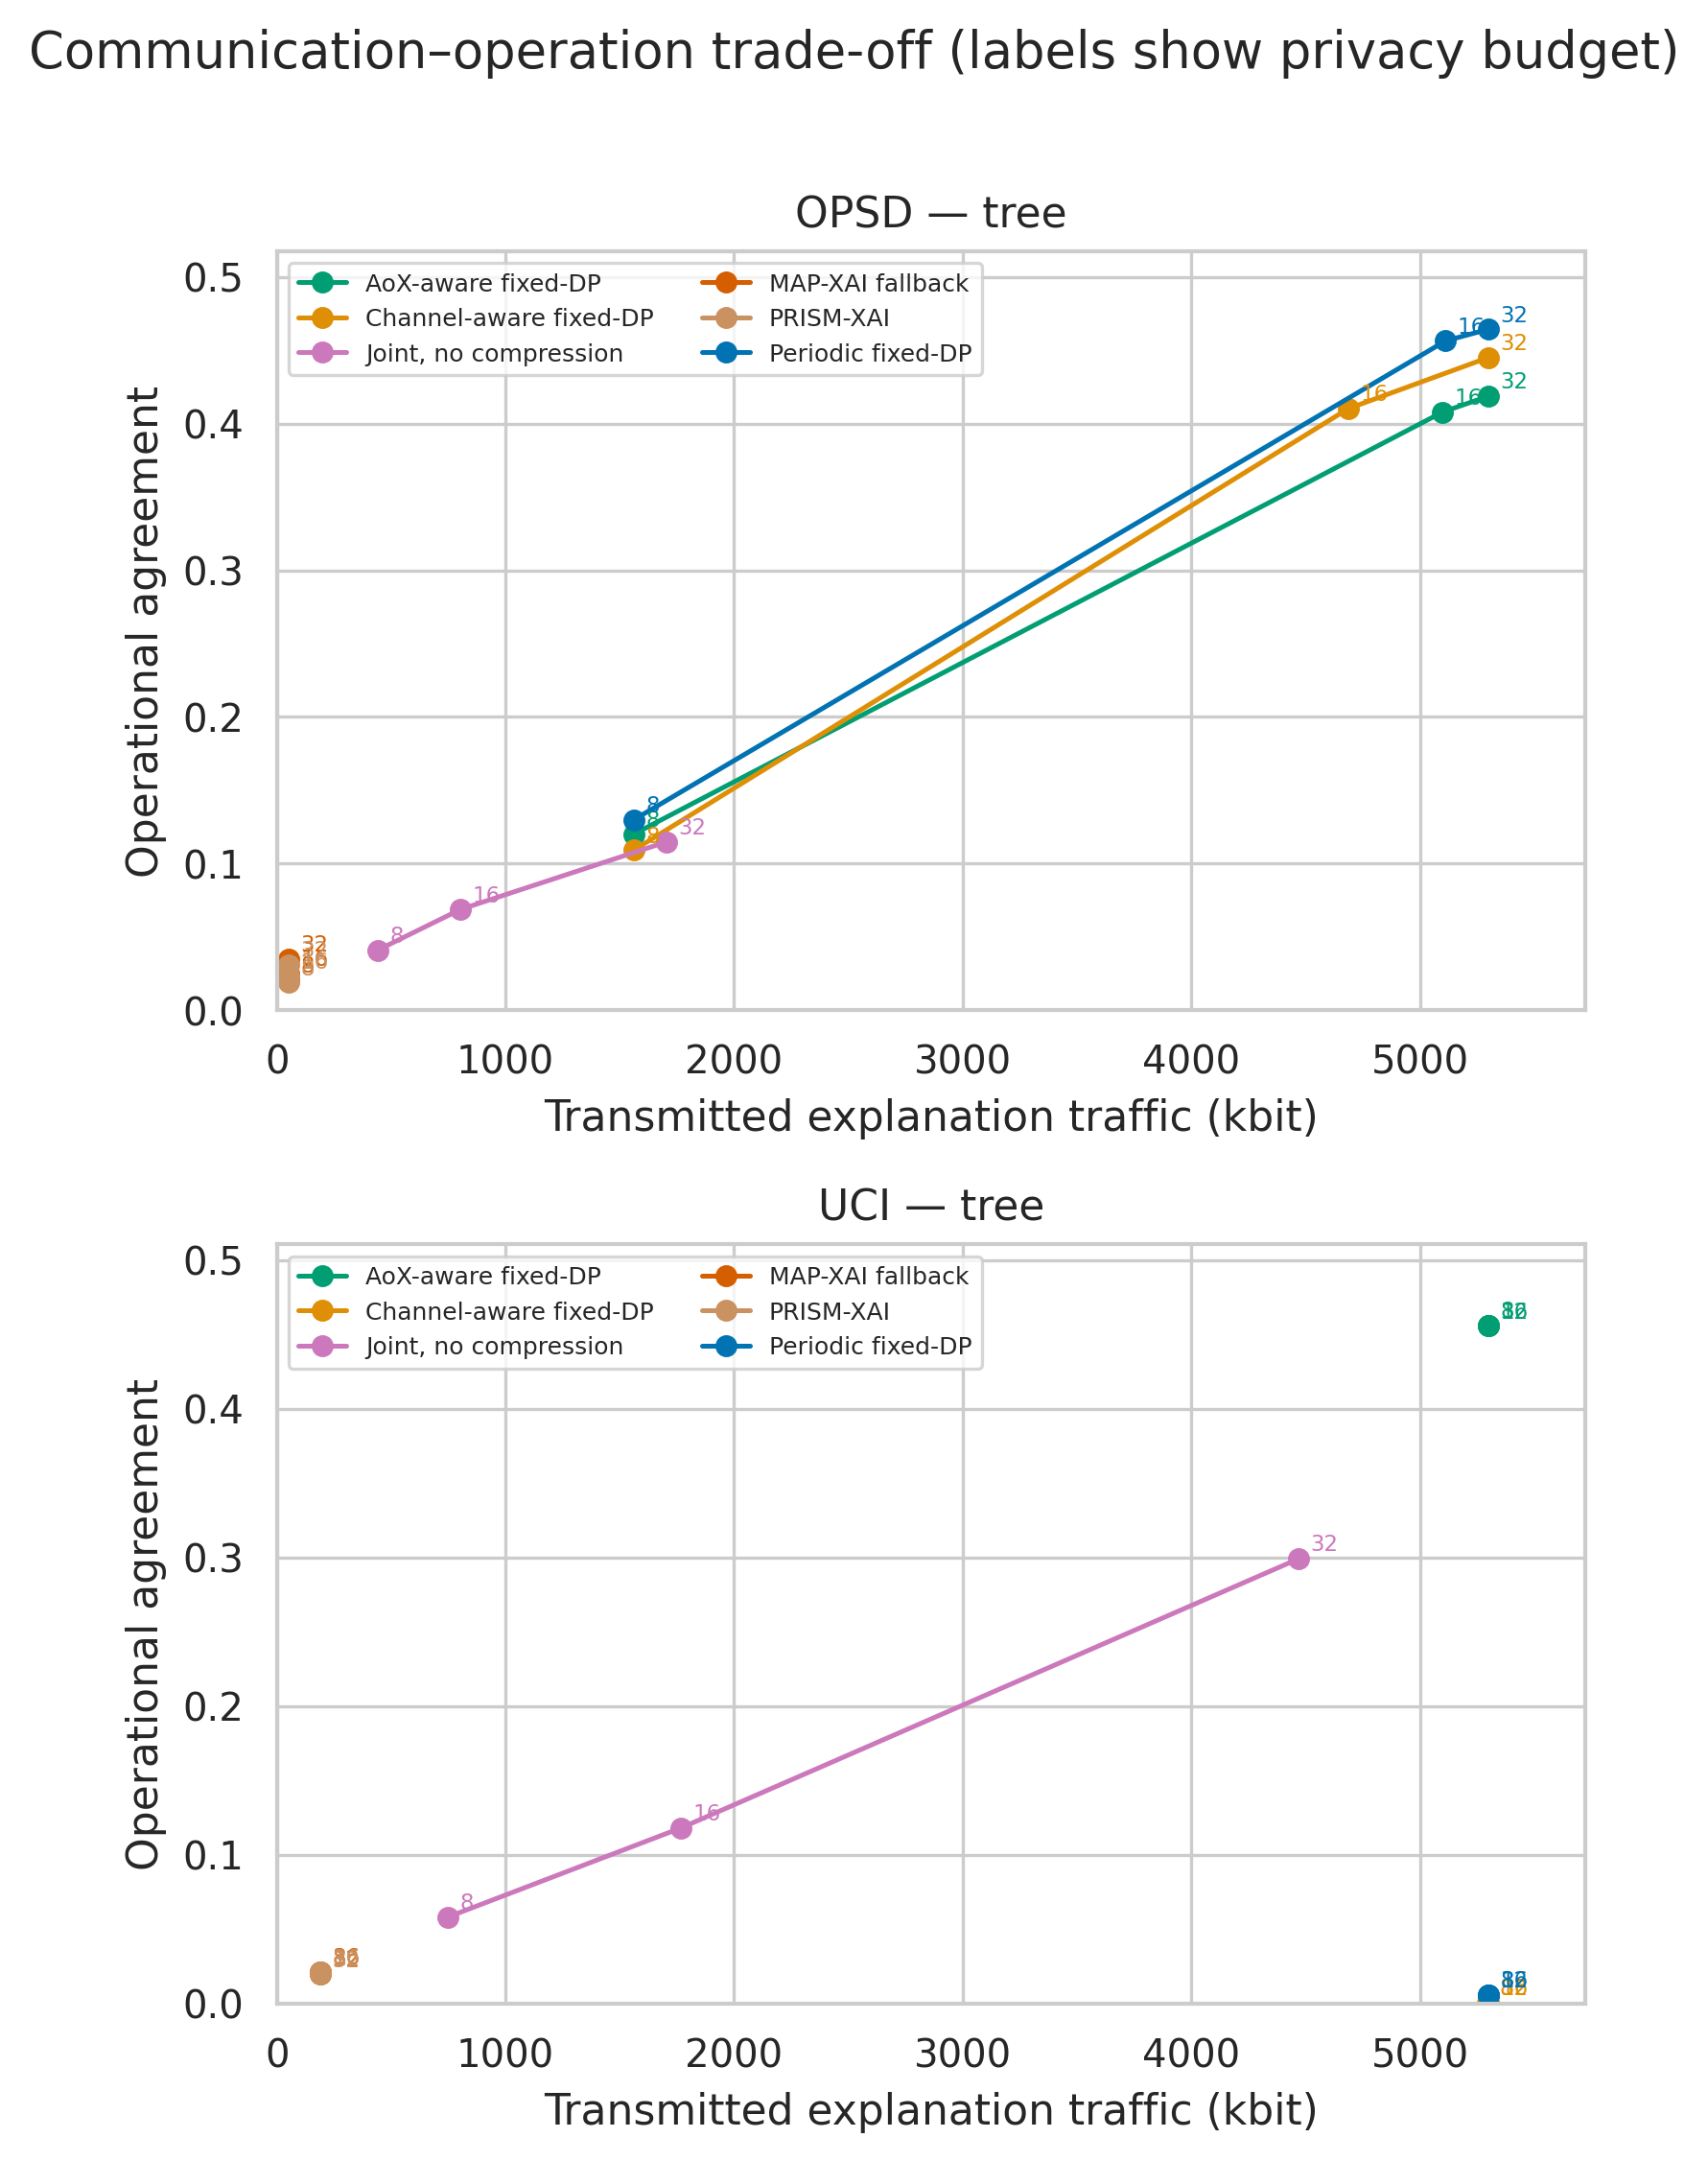
\includegraphics[width=\linewidth]{v19_M4_pareto_bits_fidelity.png}\\[-1mm]
{\small (a) M4 communication--operation}
\end{minipage}\hfill
\begin{minipage}{.49\linewidth}
\centering
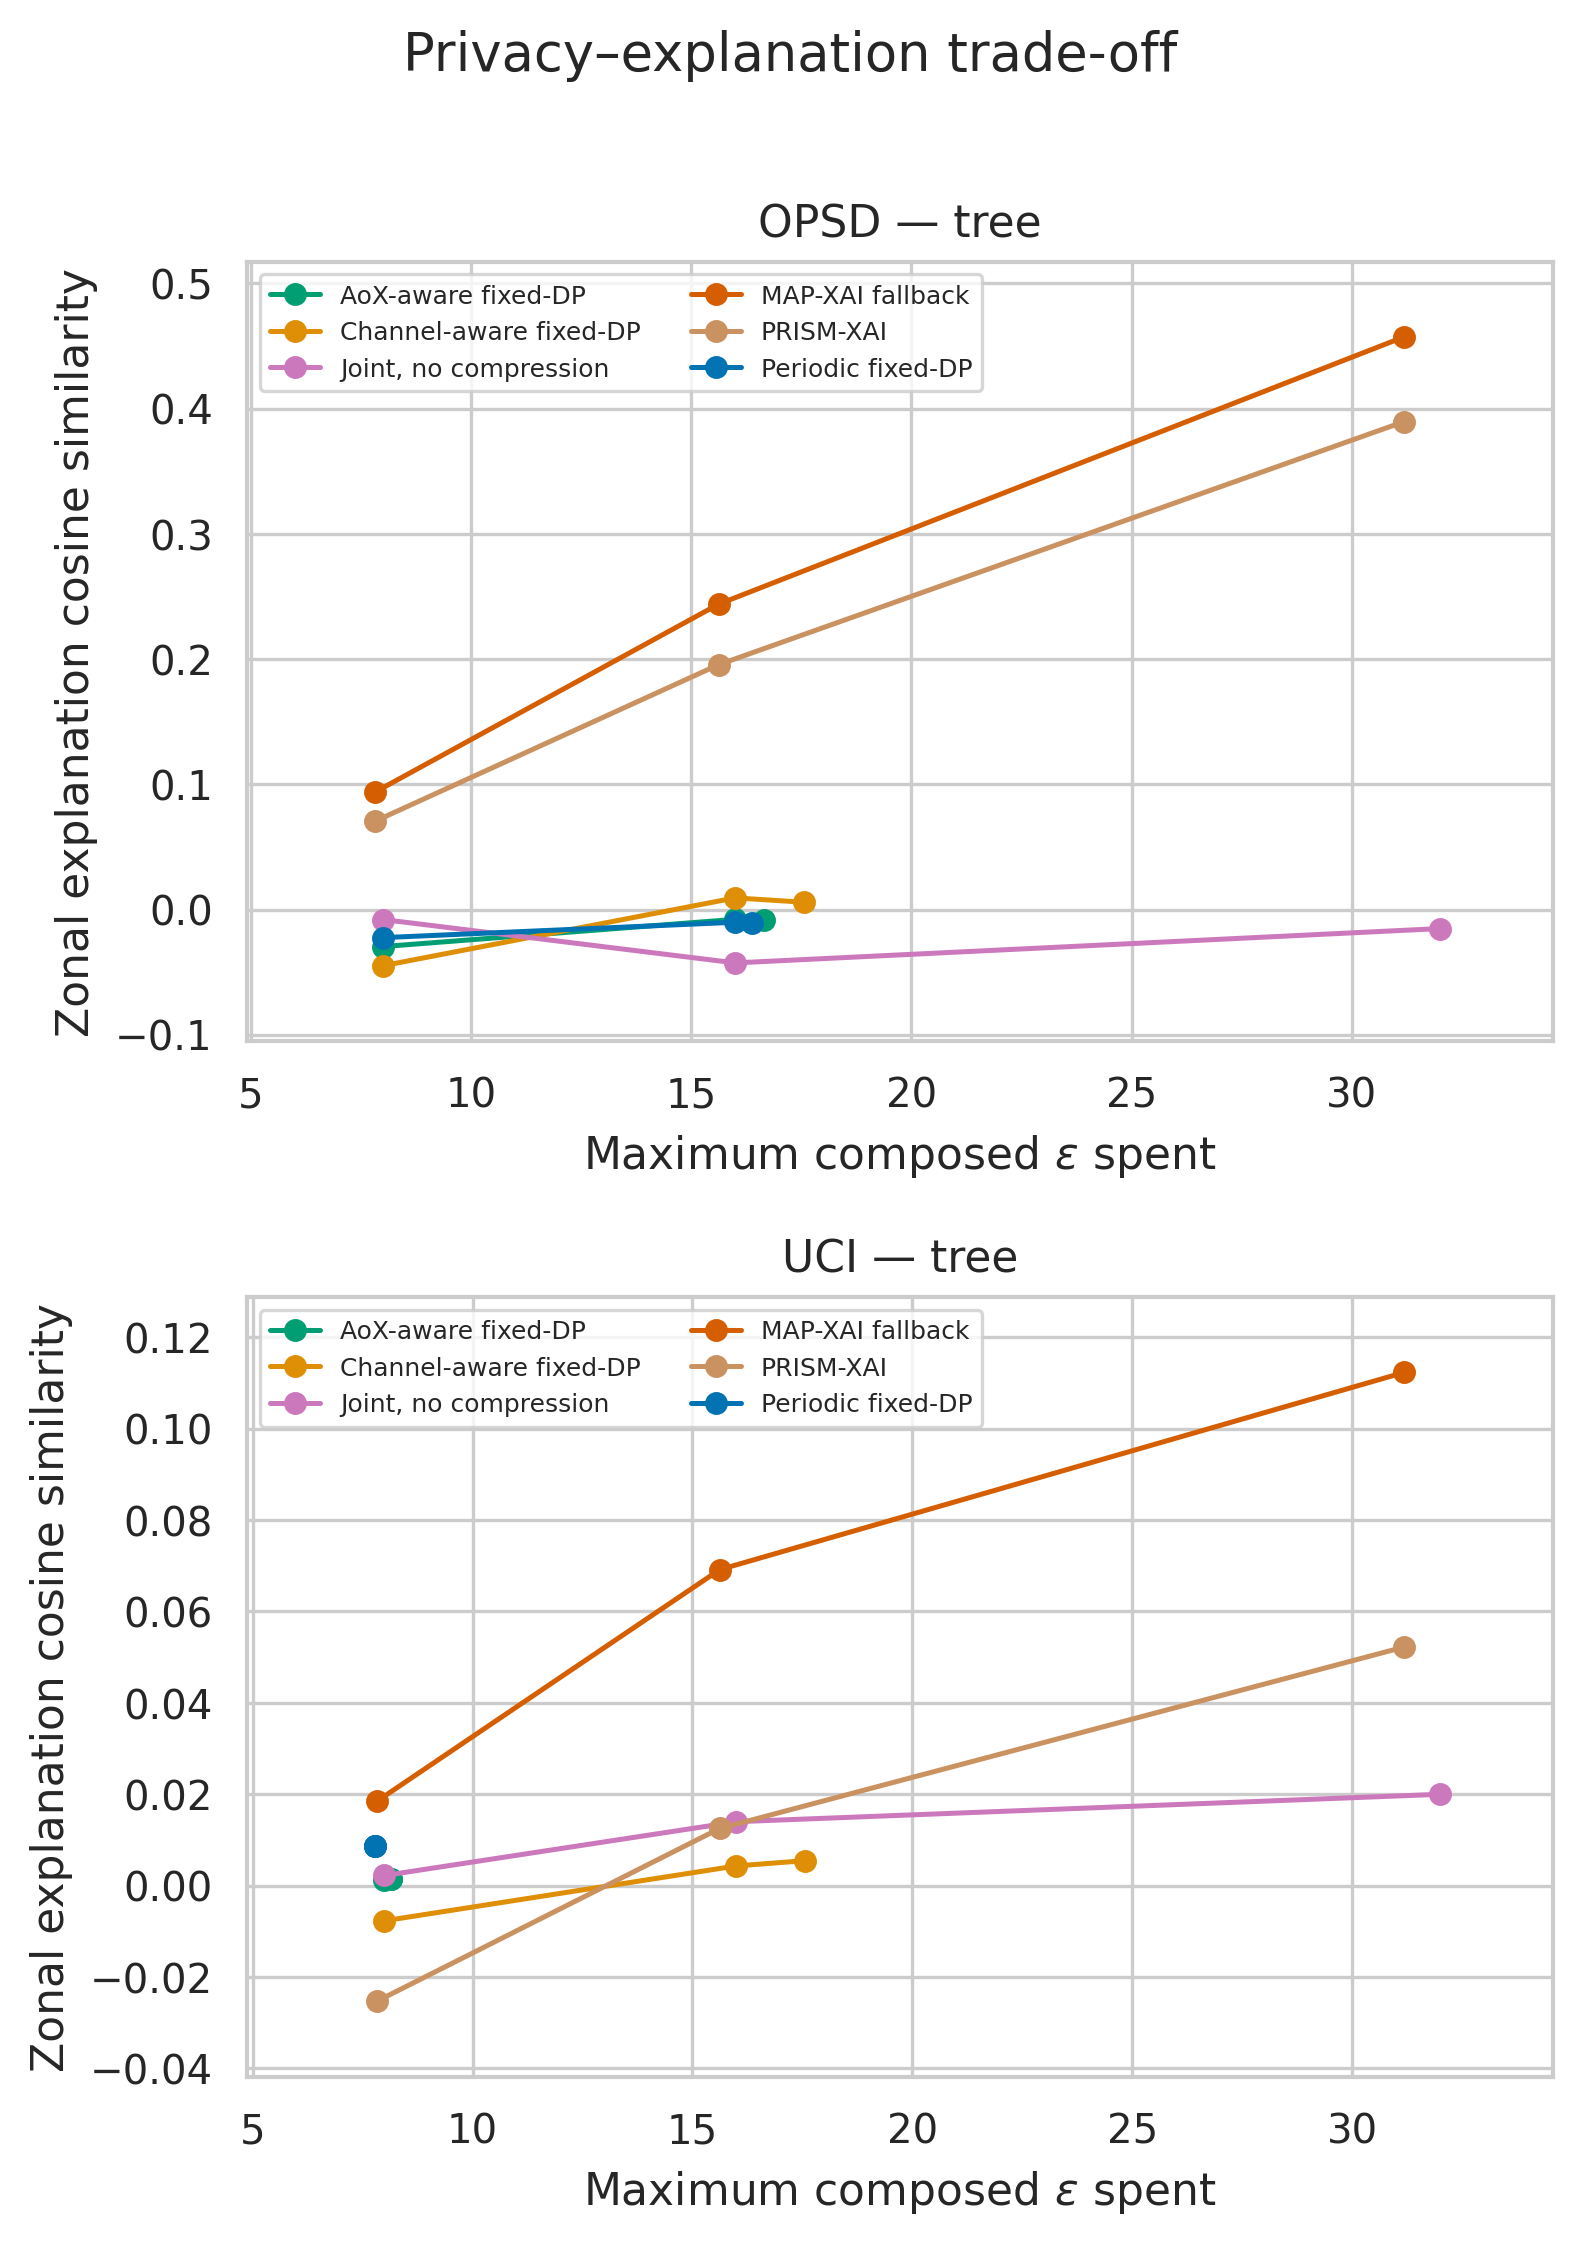
\includegraphics[width=\linewidth]{v19_M4_privacy_fidelity.png}\\[-1mm]
{\small (b) M4 privacy--fidelity}
\end{minipage}
\caption{v19 M4 sensitivity. The tighter release cap further reduces communication and can improve fidelity or intervention precision among the small number of accepted releases, but most PRISM-XAI runs no longer satisfy the configured critical-event coverage floor.}
\label{fig:m4_pareto}
\end{figure}

Figure~\ref{fig:m4_pareto} visualizes the same trade-off: the tighter cap reduces communication and concentrates the accepted releases, but leaves a larger fraction of critical periods without fresh explanation service.

\subsection{Fairness and Temporal Behavior under M4}

\begin{figure}[htbp]
\centering
\begin{minipage}{.49\linewidth}
\centering
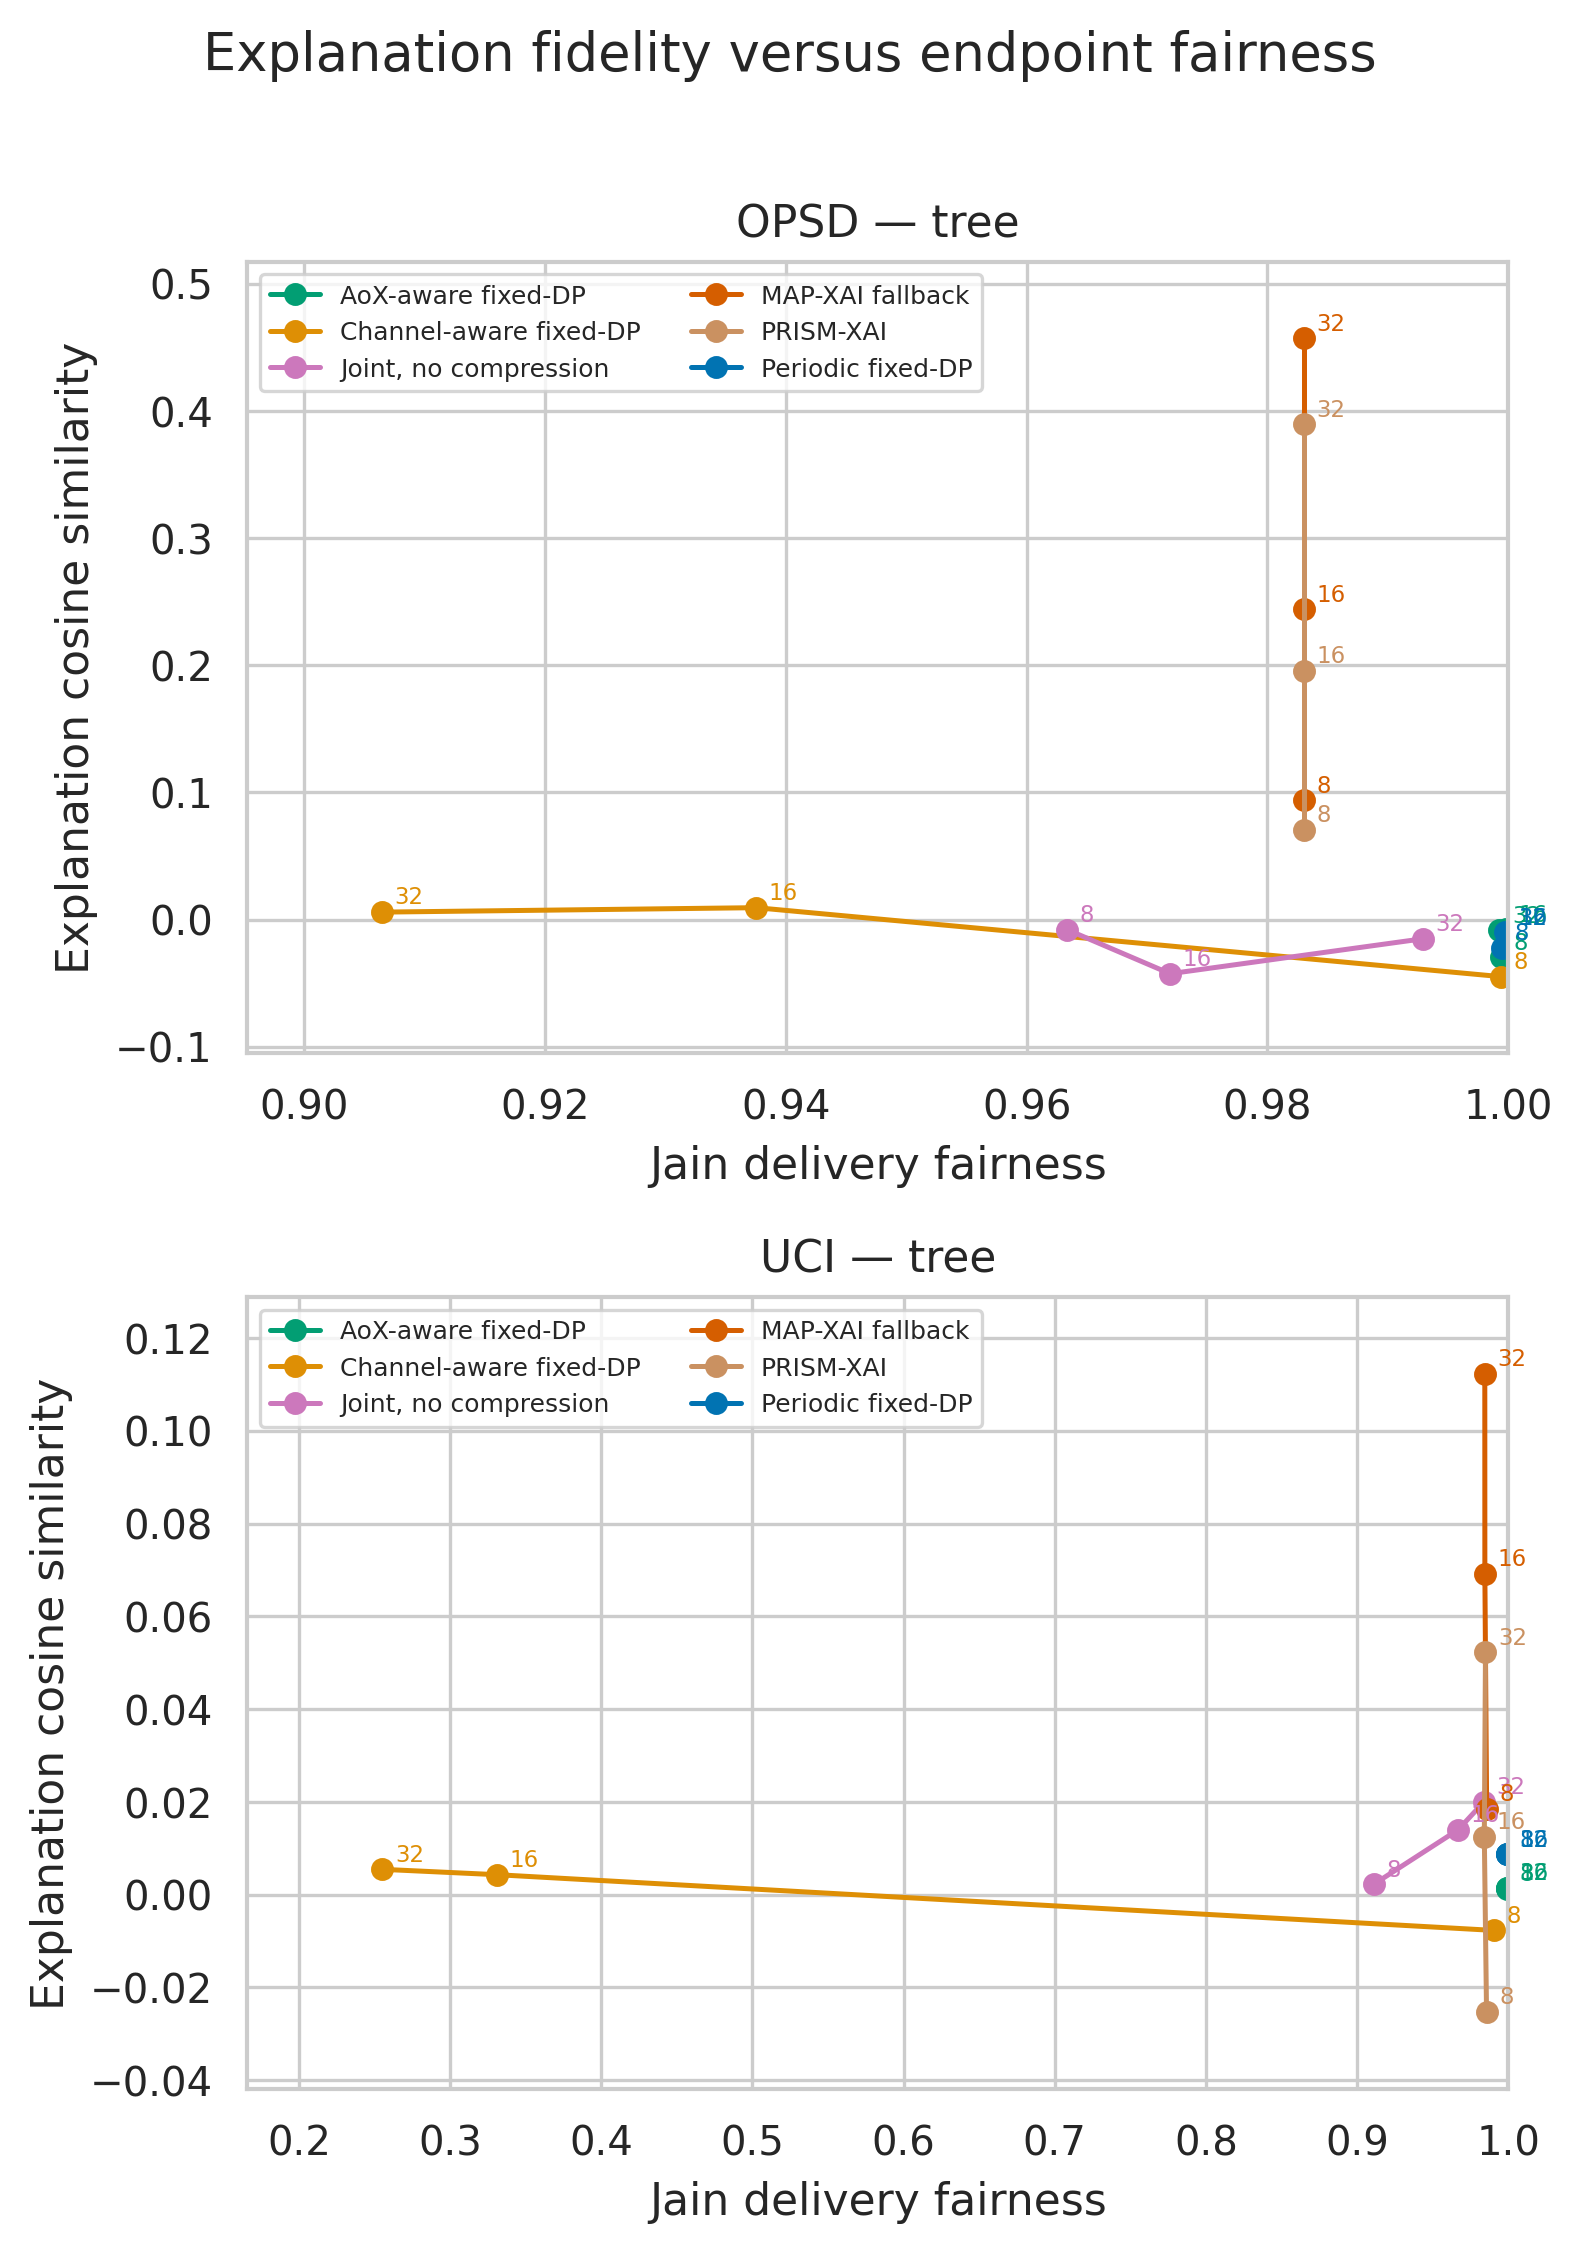
\includegraphics[width=\linewidth]{v19_M4_fairness_reliability.png}
{\small (a) M4 fairness--fidelity}
\end{minipage}\hfill
\begin{minipage}{.49\linewidth}
\centering
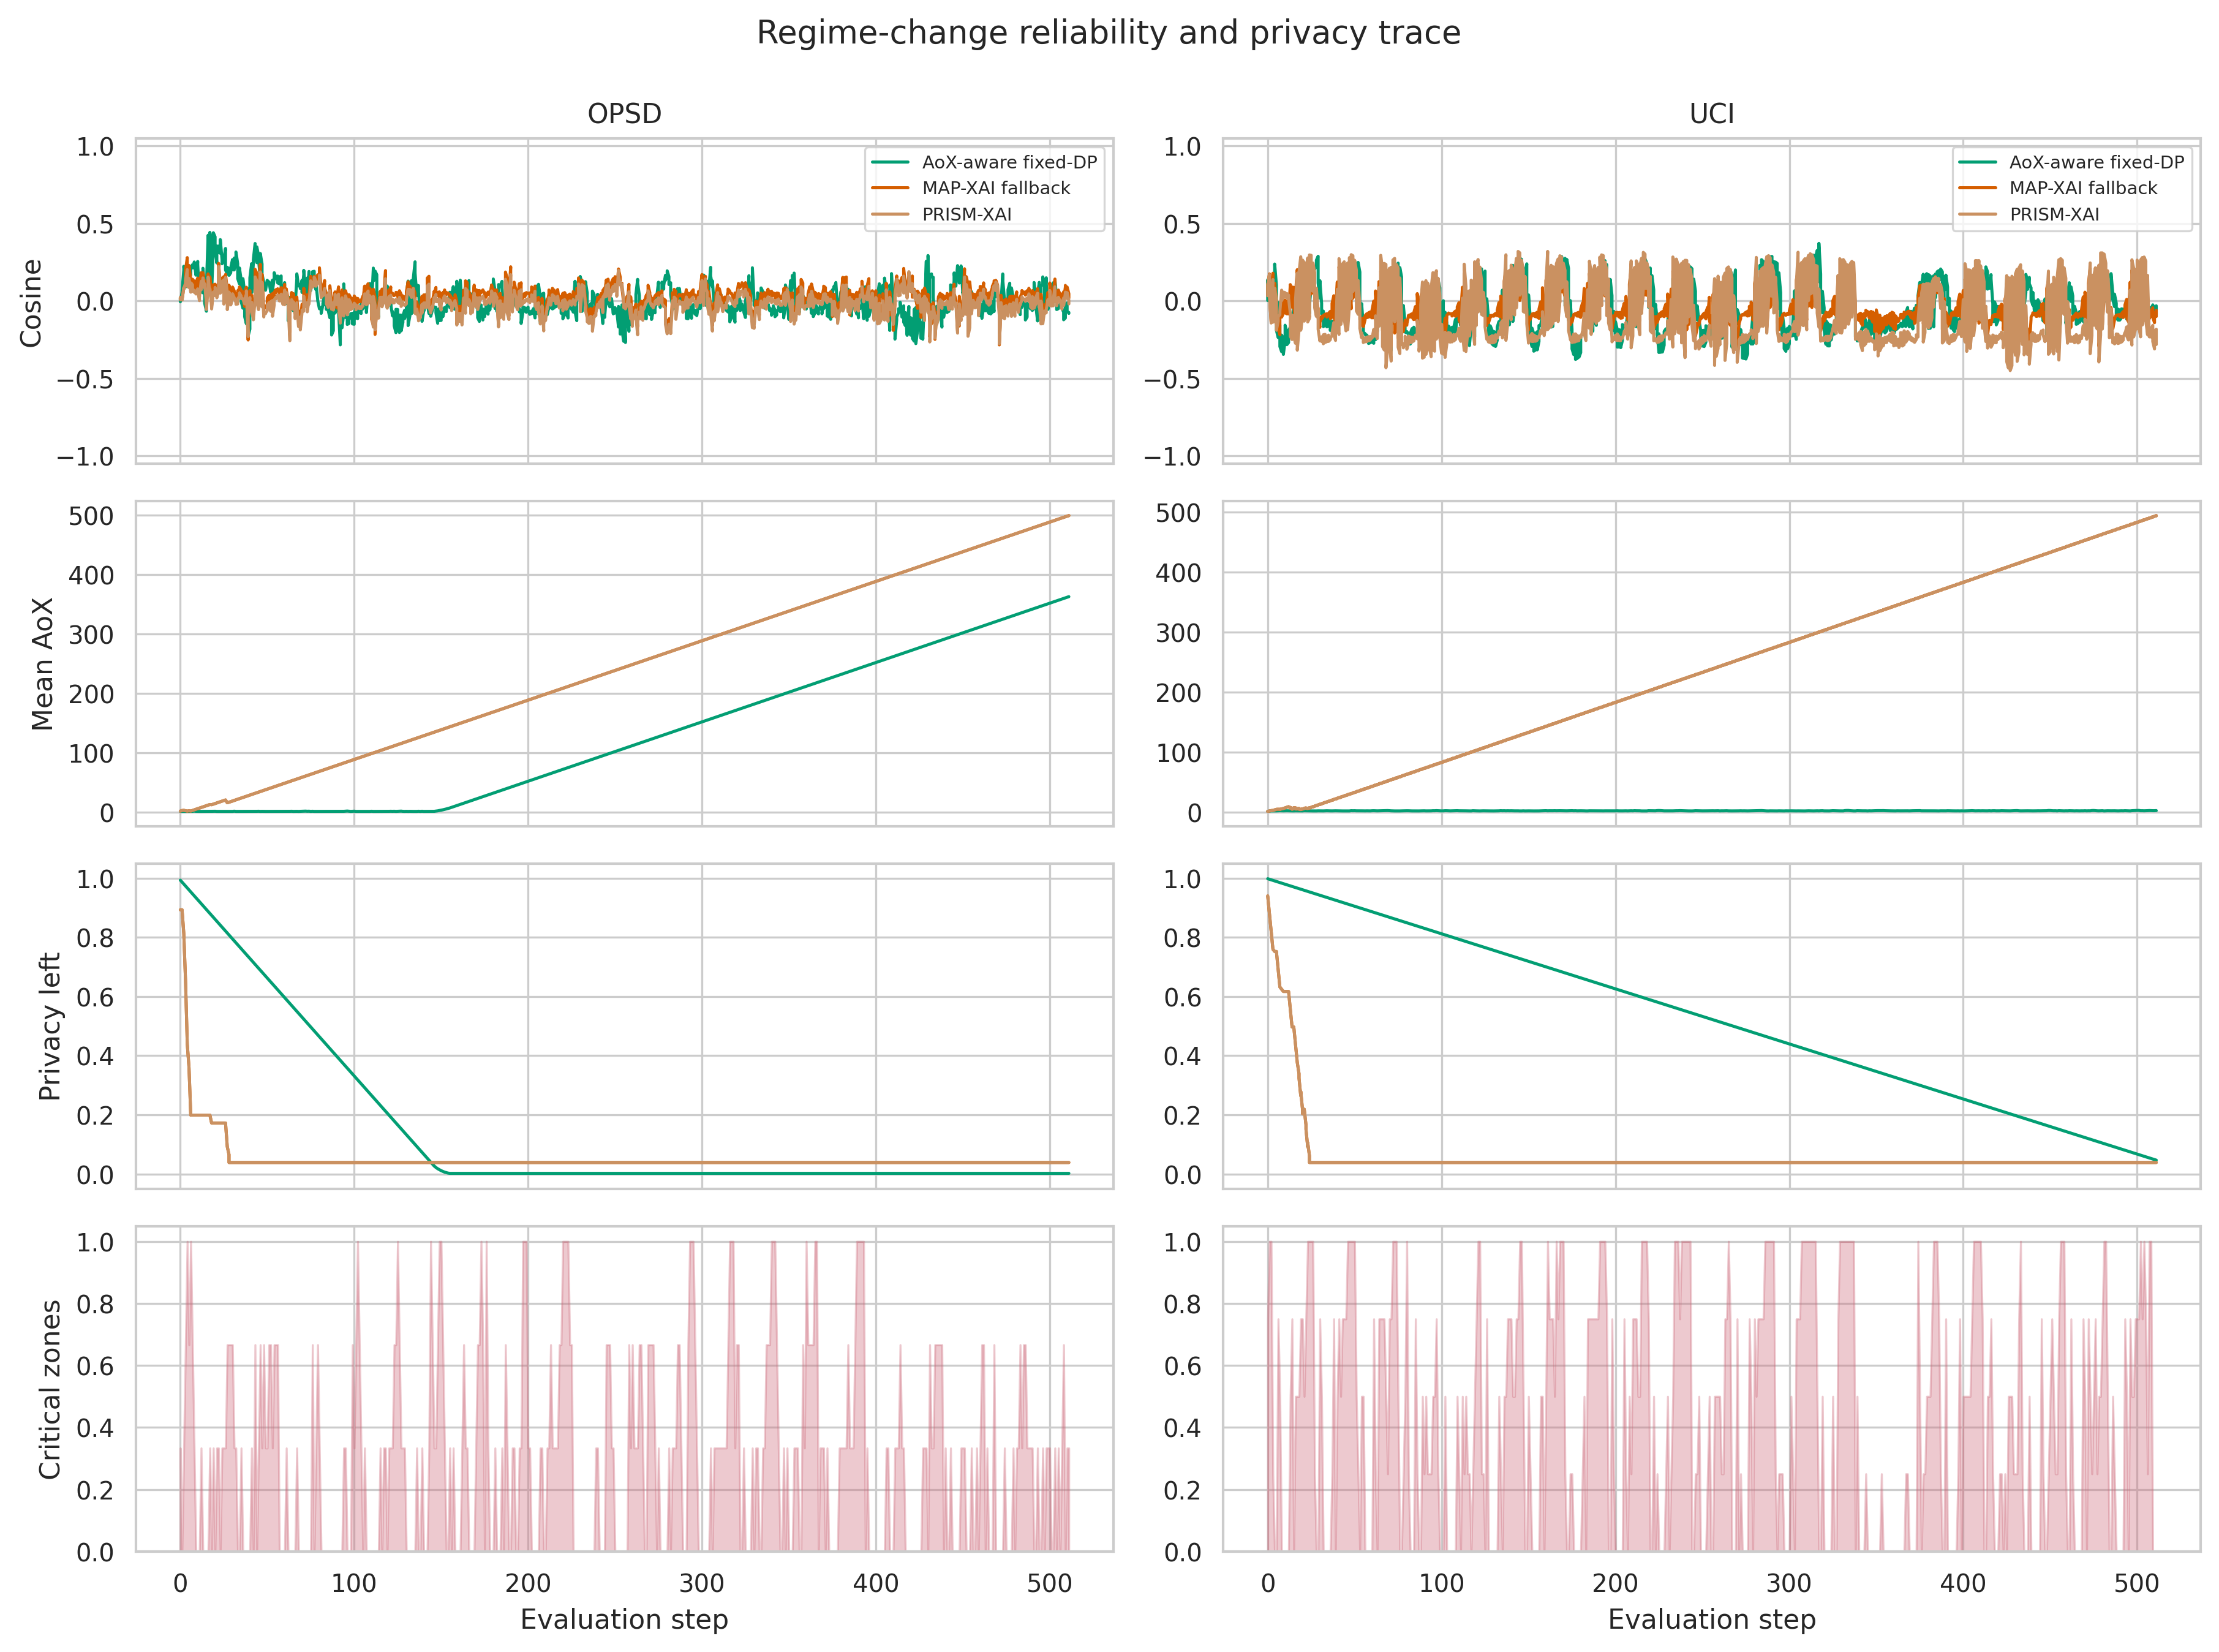
\includegraphics[width=\linewidth]{v19_M4_regime_trace.png}
{\small (b) M4 representative trace}
\end{minipage}
\caption{Additional v19 M4 sensitivity evidence. The tighter release cap preserves high average fairness but produces a sparser service process and consumes the small number of useful private-release opportunities earlier in the evaluation horizon.}
\label{fig:m4_fairness_trace}
\end{figure}

The fairness and temporal results in Fig.~\ref{fig:m4_fairness_trace} reinforce the same interpretation. Average endpoint fairness remains high, indicating that M4 does not simply concentrate all transmissions on a small subset of endpoints. Nevertheless, the lower minimum fairness shows that the reduced number of available updates leaves less flexibility to correct service imbalance in difficult stochastic realizations.

The representative M4 trace also shows that the four-release allowance is exhausted more quickly than under M8. Once these opportunities have been used, AoX grows and later critical events remain uncovered. This temporal mechanism explains why M4 fails the coverage guardrail even though the transmissions that do occur can exhibit favorable precision or fidelity.

\subsection{Selection of M8 as the Main Operating Point}

M8 is selected as the principal v19 operating point because it retains the substantial efficiency gains of selective private explanation delivery while satisfying the predefined critical-event coverage requirement in every main PRISM-XAI run. M4 is more communication-efficient and more precise among accepted releases, but it violates that service guardrail in most runs.

The comparison therefore treats the release cap as an operational design parameter rather than a quantity to minimize: additional selectivity is useful only while the declared service requirement remains satisfied.

\section{Feasibility Ladder: Locating the Explanation-Fidelity Bottleneck}

The final M8 results combine several transformations: attribution clipping, differential-privacy perturbation, semantic compression, and selective scheduling. Observing only the final PRISM-XAI output therefore does not identify which stage is responsible for the degradation in explanation fidelity. The feasibility ladder separates these transformations sequentially so that the dominant source of information loss can be localized.

The ladder contains six stages. Stages A--D isolate the representation and privacy pipeline before selective online scheduling is introduced, whereas Stages E--F add the proposed selective delivery mechanisms. This separation makes it possible to distinguish \emph{explanation-fidelity loss} from \emph{service and communication reduction}.

Conceptually, the ladder is

$$
\text{A: oracle explanation}
\rightarrow
\text{B: clipping}
\rightarrow
\text{C: private full explanation}
\rightarrow
\text{D: private compressed explanation}
\rightarrow
\text{E: MAP-XAI-only}
\rightarrow
\text{F: PRISM-XAI}.
$$

Each transition therefore introduces one additional component of the complete processing chain. If a large performance change first appears between two consecutive stages, that transition identifies the mechanism primarily responsible for the change.

\small

\setlength{\tabcolsep}{3pt}
\renewcommand{\arraystretch}{1.08}
\begin{longtable}{llrrrrrrr}
\caption{Complete feasibility-ladder summary at $\epsilon_{\max}=4$ (three seeds).}\label{tab:ladderfull}\\
\toprule
Data & Stage & Cosine & Top-K & Recall & Coverage & kbit & eps spent & Rand.Top-K \\
\midrule
\endfirsthead
\toprule
Data & Stage & Cosine & Top-K & Recall & Coverage & kbit & eps spent & Rand.Top-K \\
\midrule
\endhead
\midrule
\multicolumn{9}{r}{Continued on next page} \\
\endfoot
\bottomrule
\endlastfoot
OPSD & A Oracle & 1.000 & 1.000 & 1.000 & 1.000 & 0.000 & 0.000 & 0.250 \\
OPSD & B Clipped & 0.993 & 0.990 & 0.969 & 1.000 & 5,879.8 & 0.000 & 0.250 \\
OPSD & C Private full & 0.025 & 0.241 & 0.368 & 0.830 & 735.0 & 4.000 & 0.250 \\
OPSD & D Private compressed & 0.023 & 0.252 & 0.357 & 0.830 & 687.2 & 4.000 & 0.250 \\
OPSD & E MAP-XAI-only & 0.003 & 0.284 & 0.012 & 0.034 & 36.85 & 3.703 & 0.250 \\
OPSD & F PRISM-XAI & 0.000 & 0.246 & 0.020 & 0.034 & 34.90 & 3.703 & 0.250 \\
UCI & A Oracle & 1.000 & 1.000 & 1.000 & 1.000 & 0.000 & 0.000 & 0.250 \\
UCI & B Clipped & 0.999 & 0.993 & 0.988 & 1.000 & 20,906 & 0.000 & 0.250 \\
UCI & C Private full & -0.020 & 0.282 & 0.241 & 0.535 & 2,613.2 & 4.000 & 0.250 \\
UCI & D Private compressed & -0.017 & 0.295 & 0.234 & 0.535 & 2,443.3 & 4.000 & 0.250 \\
UCI & E MAP-XAI-only & 0.023 & 0.260 & 0.008 & 0.018 & 115.8 & 3.703 & 0.250 \\
UCI & F PRISM-XAI & 0.030 & 0.222 & 0.009 & 0.018 & 114.0 & 3.703 & 0.250 \\
\end{longtable}

\subsection{Stage A to Stage B: Clipping Preserves the Explanation Structure}

Stage A is the non-private oracle explanation and therefore has Top-$K$ agreement and cosine similarity equal to \(1\) by construction. Stage B applies the clipping operation required to bound sensitivity before differential privacy is introduced.

The effect of clipping is very small. On OPSD, Top-$K$ agreement decreases only from \(1.000\) to \(0.990\), while cosine similarity remains \(0.993\). On UCI, Top-$K$ remains \(0.993\) and cosine similarity remains \(0.999\). Critical-event recall also remains high, at approximately \(0.969\) for OPSD and \(0.988\) for UCI.

These results show that the clipping operation preserves almost all of the original attribution structure. Both the identities of the dominant features and the direction of the complete attribution vector remain close to the non-private oracle.

This observation is important because clipping is the first modification applied to the original explanation. If clipping had already destroyed the attribution structure, subsequent fidelity losses could not be attributed specifically to differential privacy. The near-unity Top-$K$ and cosine values demonstrate that this is not the case.

Thus, the transition

$$
\text{oracle}
\rightarrow
\text{clipped explanation}
$$

introduces negligible fidelity degradation and is not the primary explanation bottleneck.

\subsection{Stage B to Stage C: Differential Privacy Produces the Dominant Fidelity Collapse}

The largest fidelity change in the entire ladder occurs when the clipped explanation is converted into a household-level differentially private release.

For OPSD, Top-$K$ agreement falls from approximately \(0.990\) after clipping to \(0.241\) after the Gaussian private mechanism. For UCI, it falls from approximately \(0.993\) to \(0.282\).

The random Top-$K$ reference for the evaluated explanation dimension is \(0.25\). Consequently, the private OPSD explanation is approximately at the random-overlap level, while the UCI result is only modestly above it.

The cosine-similarity change is equally strong. OPSD decreases from \(0.993\) to approximately \(0.025\), while UCI decreases from \(0.999\) to approximately \(-0.020\). The private attribution vectors therefore retain very little directional agreement with the corresponding oracle explanations.

The transition

$$
\text{clipped explanation}
\rightarrow
\text{private full explanation}
$$

is consequently the first stage at which explanation fidelity collapses.

This result identifies cumulative household-level differential privacy as the dominant fidelity limitation in the evaluated configuration. The loss occurs before semantic compression and before either MAP-XAI or PRISM-XAI makes a selective transmission decision.

This distinction explains why modifications to scheduler weights cannot by themselves recover high oracle agreement. The online scheduler receives explanation information that has already undergone substantial privacy perturbation. Scheduling can decide whether that information is sufficiently valuable to transmit, but it cannot reconstruct attribution structure that has already been removed by the private mechanism.

The result therefore separates the \emph{privacy problem} from the \emph{scheduling problem}: the low explanation similarity observed in the final system originates primarily in the private release stage rather than in the scheduler.

\subsection{Stage C to Stage D: Semantic Compression Introduces Little Additional Fidelity Loss}

Stage D applies semantic compression to the already-private explanation. This transition isolates whether Top-\(k\) selection, quantization, or the reduced semantic representation creates a second major fidelity bottleneck.

The results show that it does not.

On OPSD, Top-$K$ changes from \(0.241\) for the private full explanation to \(0.252\) after compression. On UCI, it changes from \(0.282\) to \(0.295\). Cosine similarity also changes only slightly.

These differences are small compared with the B-to-C transition. Most of the explanation information lost relative to the oracle has therefore already disappeared before compression is applied.

Communication decreases at this stage. OPSD traffic falls from approximately \(735.0\) kbit for the full private representation to approximately \(687.2\) kbit after compression. UCI decreases from approximately \(2613.2\) kbit to \(2443.3\) kbit.

The savings are meaningful but modest relative to the later selective-scheduling reduction. More importantly, they are obtained without a corresponding large decrease in Top-$K$ or cosine similarity.

This result supports the design of MAP-XAI's semantic packetization. Compressing an explanation \emph{after} the privacy mechanism does not create the dominant fidelity loss. The semantic representation largely preserves the information that remains available in the private explanation.

The observed final fidelity should therefore not be interpreted as evidence that Top-\(k\) packetization or quantization destroys an otherwise high-quality private explanation. The private explanation has already suffered the major degradation at Stage C.

\subsection{Stages D to E and F: Selective Scheduling Produces the Main Communication Reduction}

Stages E and F introduce selective explanation delivery.

Stage E corresponds to the MAP-XAI-only restricted configuration, while Stage F corresponds to the complete PRISM-XAI scheduling architecture. The most prominent change at these stages is not another large collapse in explanation similarity, but a sharp reduction in transmitted traffic and explanation-service frequency.

For OPSD, traffic decreases from approximately \(687.2\) kbit at the private-compressed Stage D to approximately \(36.85\) kbit under MAP-XAI-only and \(34.90\) kbit under PRISM-XAI.

For UCI, traffic decreases from approximately \(2443.3\) kbit to \(115.8\) kbit under MAP-XAI-only and \(114.0\) kbit under PRISM-XAI.

Thus, the transition from continuously available private-compressed explanations to selective semantic delivery removes most of the communication load:

$$
687.2
\rightarrow
36.85/34.90\text{ kbit}
\quad\text{on OPSD},
$$

and

$$
2443.3
\rightarrow
115.8/114.0\text{ kbit}
\quad\text{on UCI}.
$$

This is the mechanism responsible for the principal communication saving of the proposed architecture.

The same transition also reduces critical-event coverage and recall. This decrease has a different origin from the earlier fidelity collapse. The explanations are not becoming dramatically less similar to the oracle because of scheduling; instead, fewer explanation updates are being transmitted.

The corresponding fidelity and service mechanisms are synthesized after the diagnostic figures.

\subsection{MAP-XAI-Only and PRISM-XAI in the Ladder}

The final two stages are also informative about the relationship between the two proposed components.

MAP-XAI-only already reduces OPSD traffic to approximately \(36.85\) kbit and UCI traffic to approximately \(115.8\) kbit. PRISM-XAI further changes these values to approximately \(34.90\) and \(114.0\) kbit, respectively.

The comparatively small E-to-F difference is expected because MAP-XAI is part of the proposed architecture rather than an external baseline. By Stage E, privacy-accounted semantic packetization and selective private release are already active. PRISM adds adaptive scheduling over this representation rather than replacing it with an unrelated mechanism.

The ladder therefore assigns different functions to the two proposed layers. MAP-XAI produces the compact privacy-accounted semantic explanation representation and already realizes most of the reduction relative to continuously transmitted private packets. PRISM-XAI adds context-dependent allocation of those packets according to explanation age, criticality, residual evidence, channel state, deadline conditions, fairness, and remaining privacy resources.

\subsection{Top-\(K\) Evidence}

\begin{figure}[htbp]
\centering
\begin{minipage}{.49\linewidth}
\centering
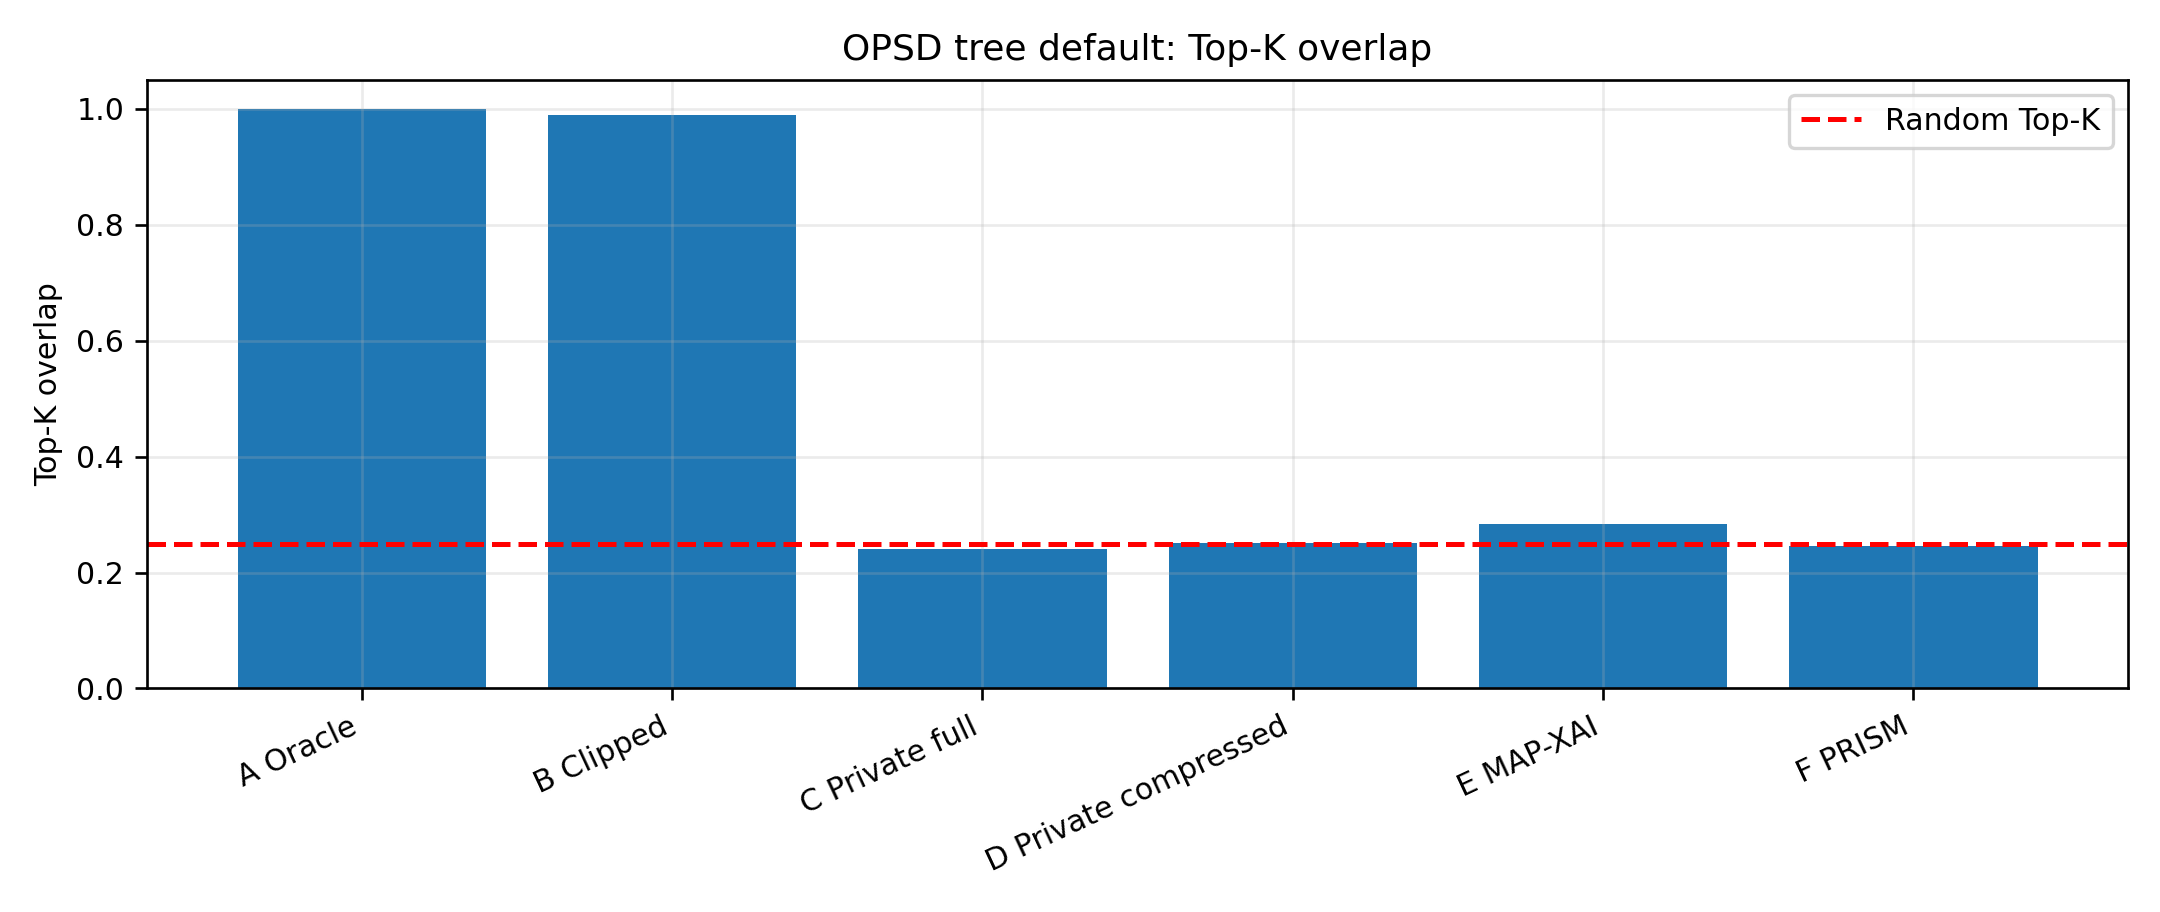
\includegraphics[width=\linewidth]{opsd_tree_default_ladder_topk.png}\\[-1mm]
{\small (a) OPSD Top-$K$}
\end{minipage}\hfill
\begin{minipage}{.49\linewidth}
\centering
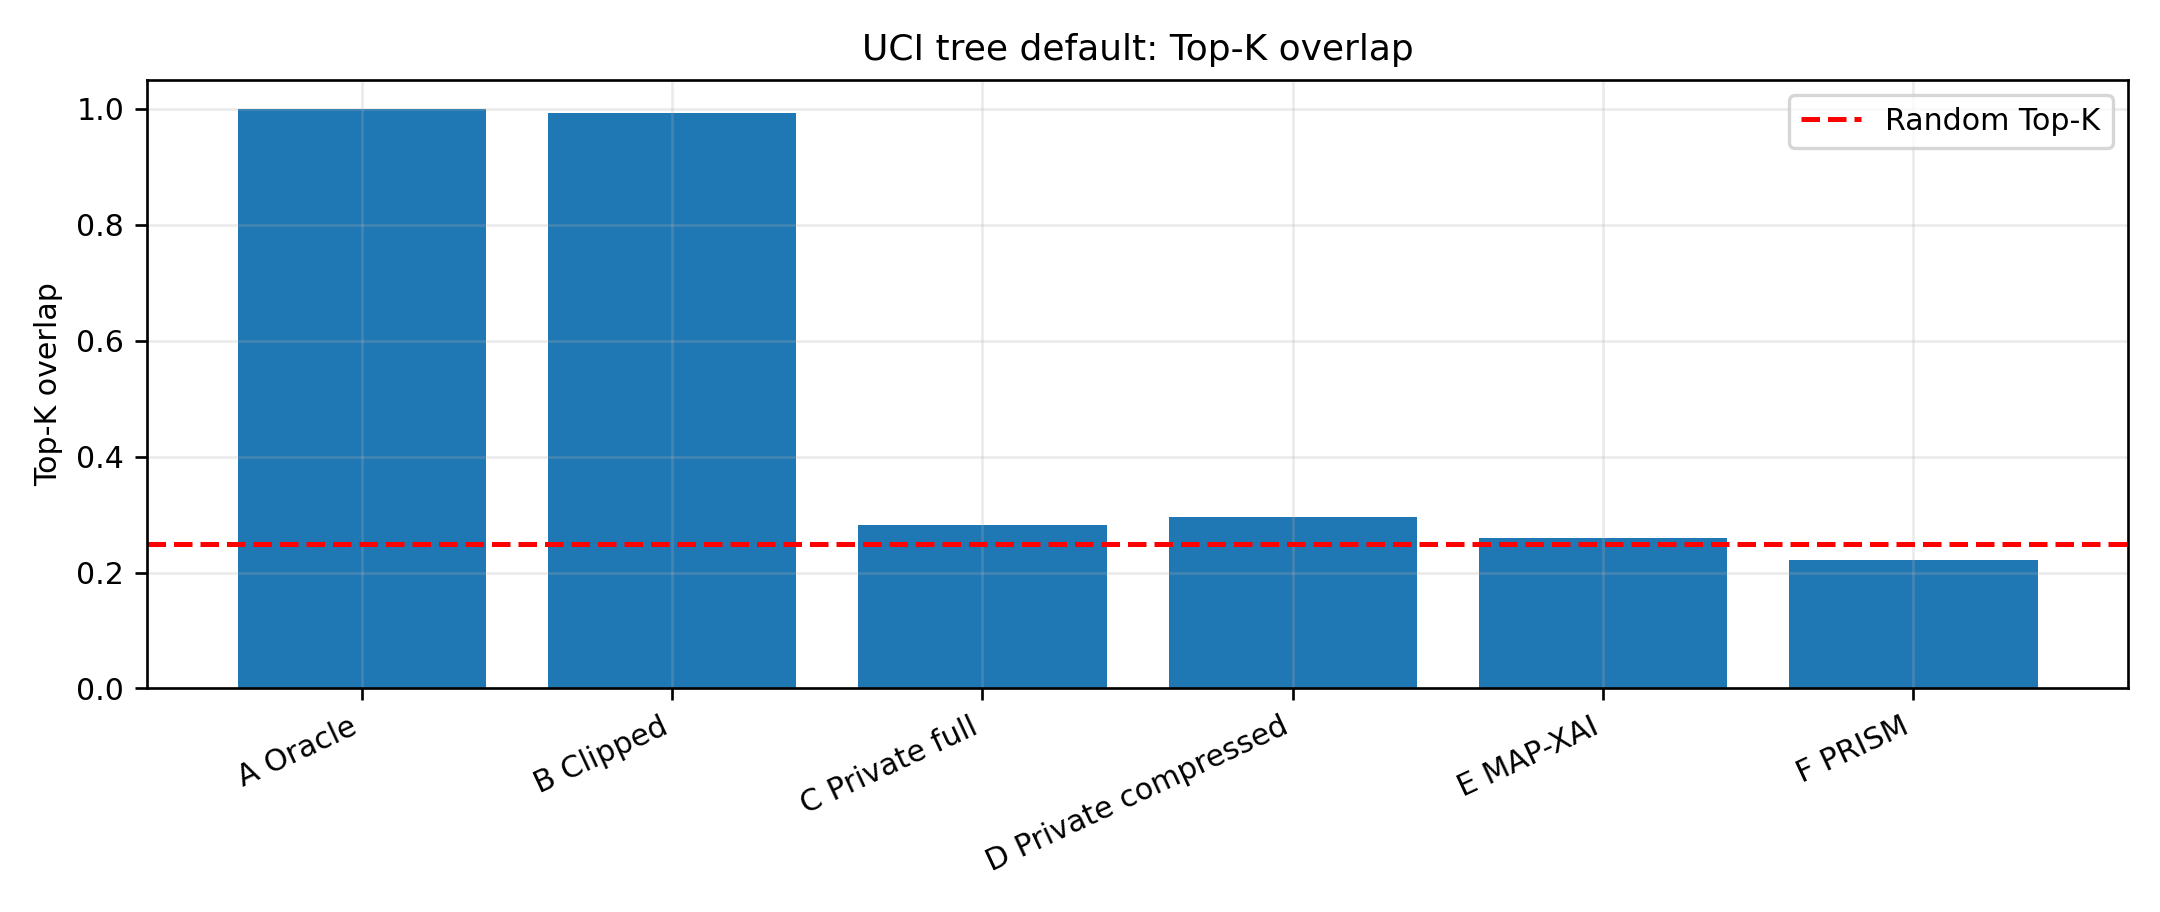
\includegraphics[width=\linewidth]{uci_tree_default_ladder_topk.png}\\[-1mm]
{\small (b) UCI Top-$K$}
\end{minipage}
\caption{Feasibility ladder for Top-$K$ agreement. Clipping preserves almost all oracle feature-ranking information, whereas the dominant collapse occurs when cumulative household-level differential privacy is introduced. Post-DP compression produces comparatively little additional degradation.}
\label{fig:ladder_topk}
\end{figure}

Figure~\ref{fig:ladder_topk} visually confirms the stage-wise Top-$K$ pattern described above: the dominant loss occurs at the private-release stage, not at clipping or post-DP compression.

\subsection{Cosine-Similarity Evidence}

\begin{figure}[htbp]
\centering
\begin{minipage}{.49\linewidth}
\centering
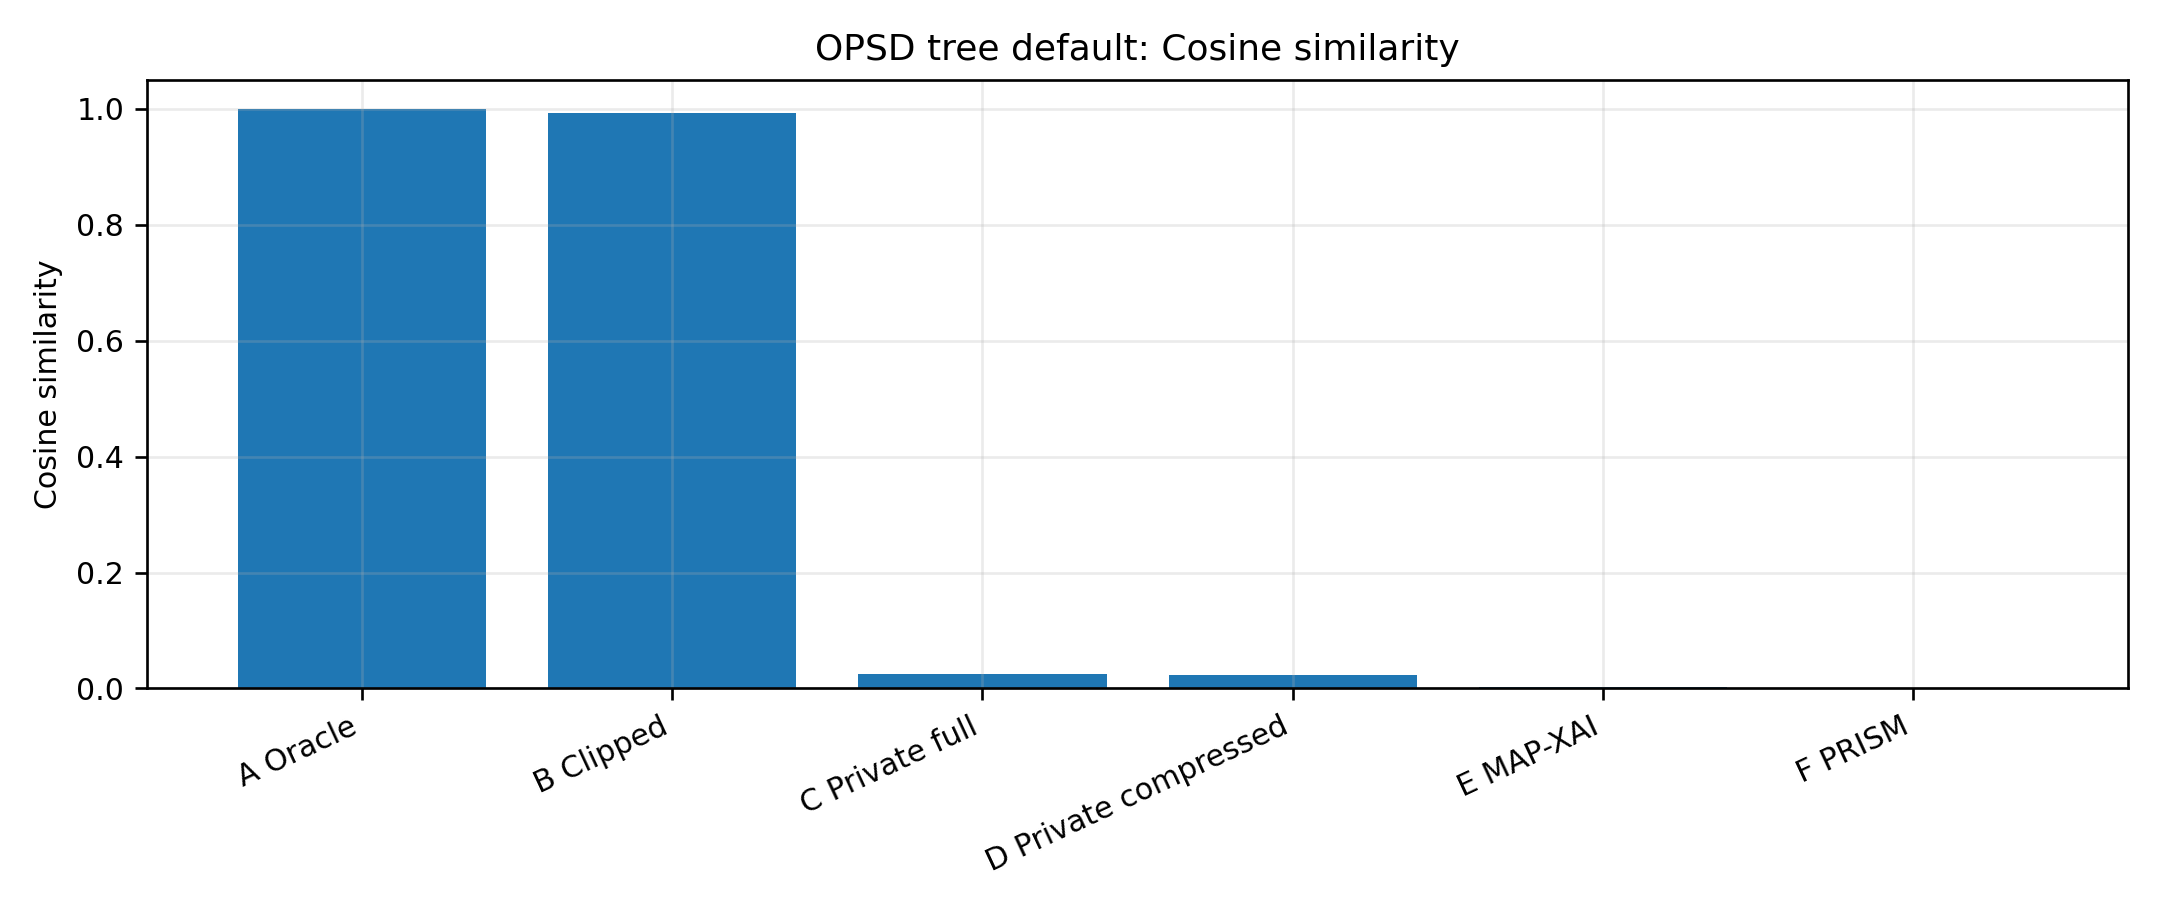
\includegraphics[width=\linewidth]{opsd_tree_default_ladder_cosine.png}\\[-1mm]
{\small (a) OPSD cosine}
\end{minipage}\hfill
\begin{minipage}{.49\linewidth}
\centering
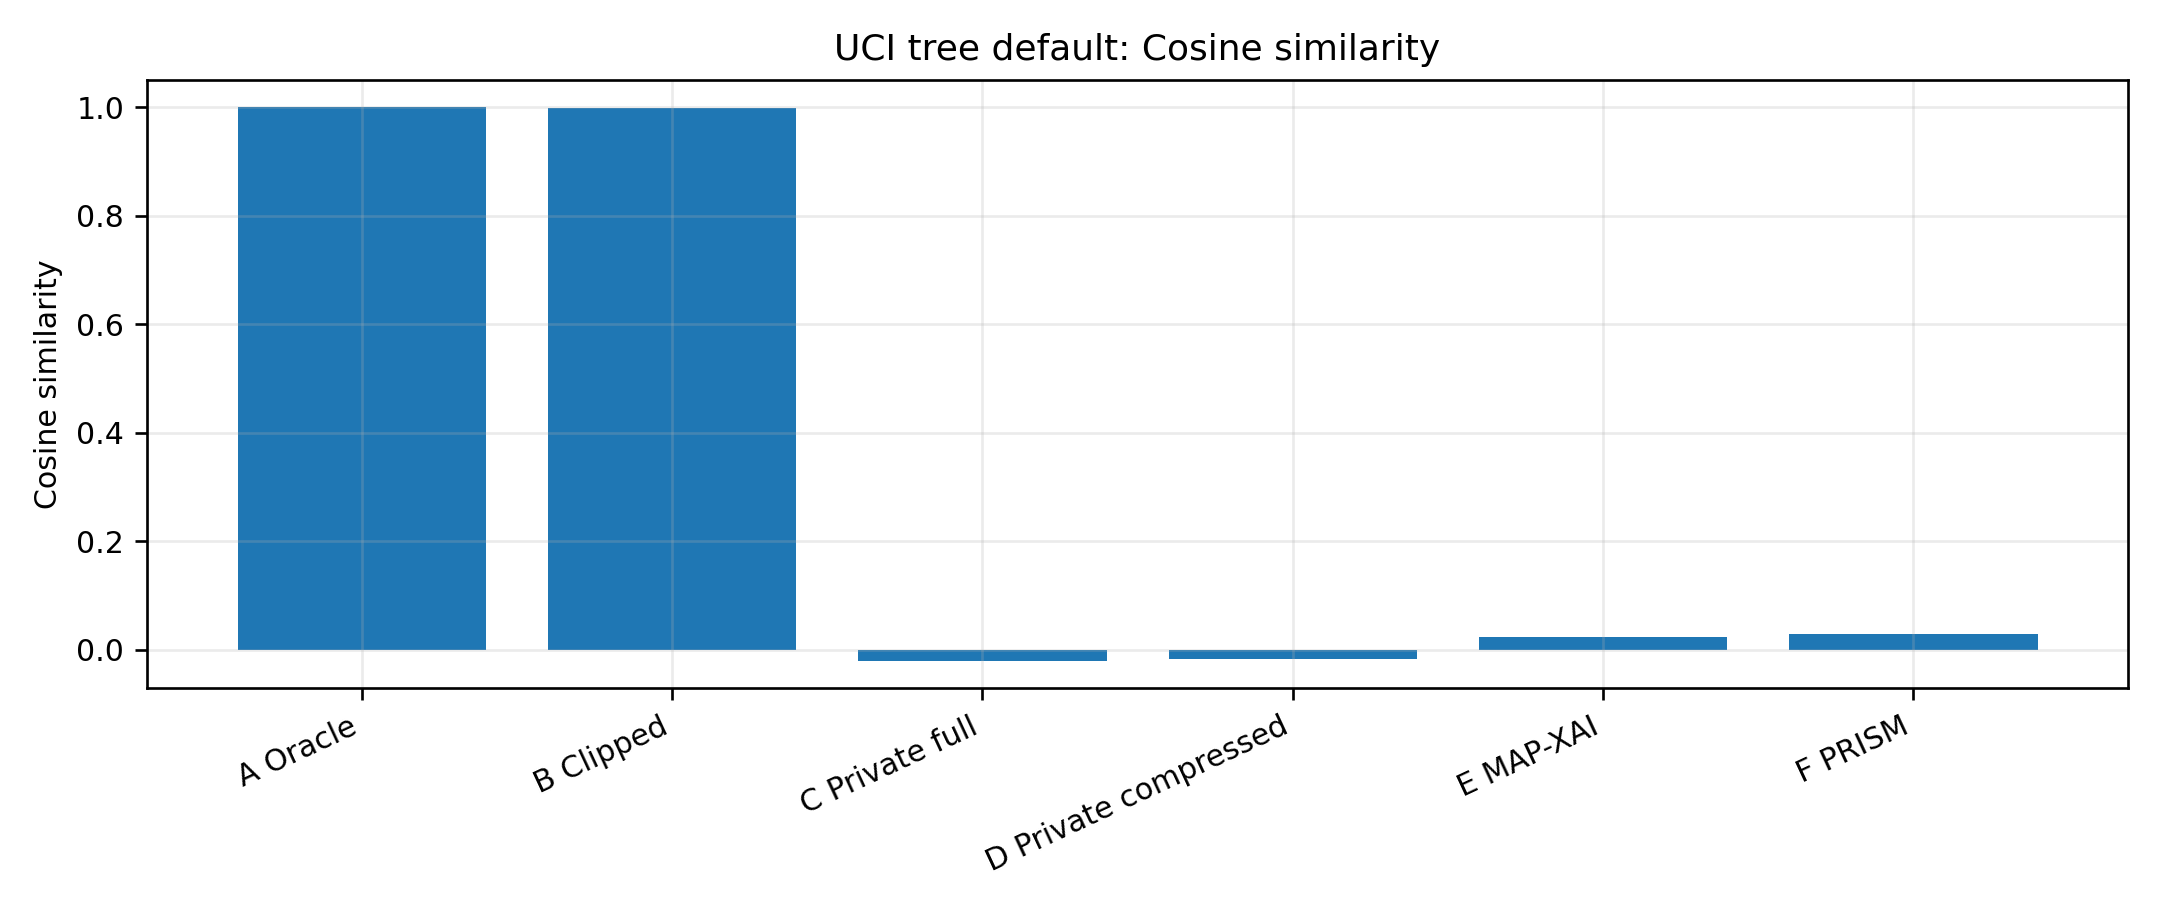
\includegraphics[width=\linewidth]{uci_tree_default_ladder_cosine.png}\\[-1mm]
{\small (b) UCI cosine}
\end{minipage}
\caption{Feasibility ladder for cosine similarity. The same privacy-driven collapse observed for Top-$K$ remains when fidelity is measured using the direction of the complete attribution vector.}
\label{fig:ladder_cosine}
\end{figure}

Figure~\ref{fig:ladder_cosine} provides the corresponding full-vector view and confirms the same diagnosis: clipping is nearly lossless, the private release drives cosine toward zero, and semantic compression adds little further change.

\subsection{Critical-Event Recall Evidence}

\begin{figure}[htbp]
\centering
\begin{minipage}{.49\linewidth}
\centering
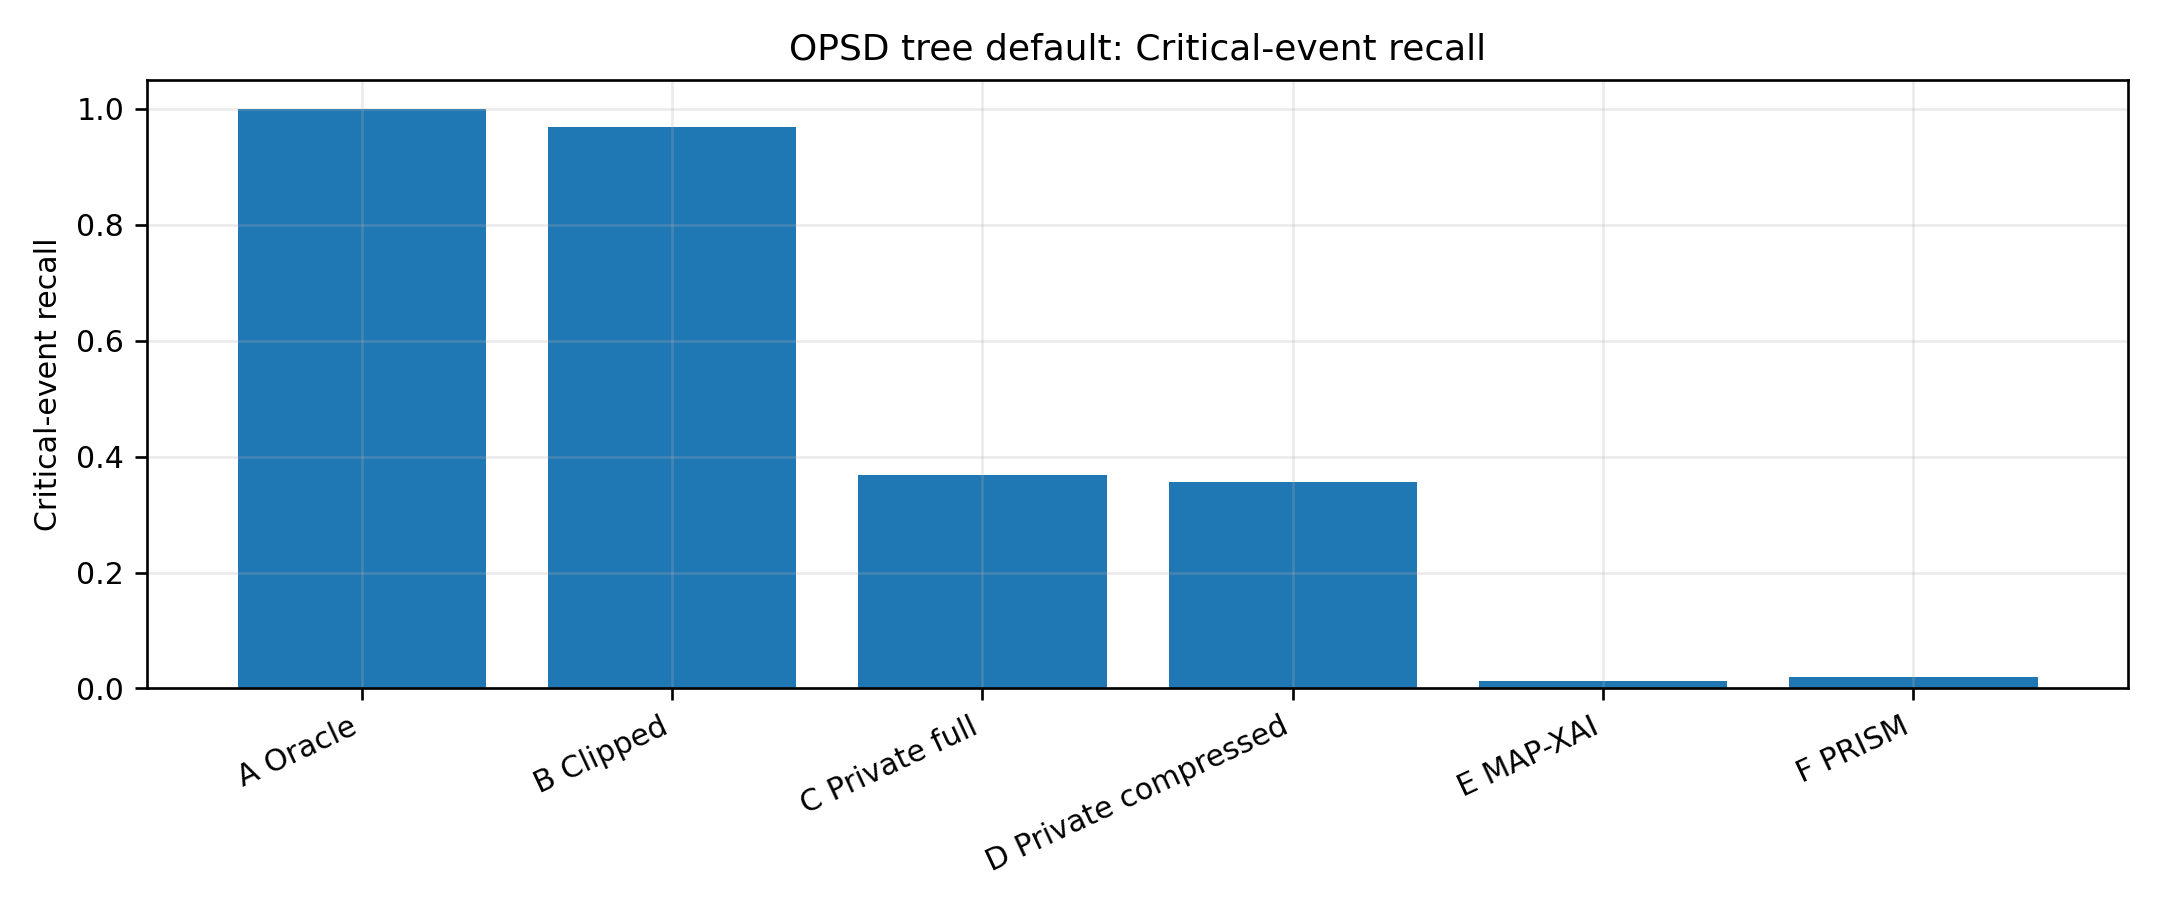
\includegraphics[width=\linewidth]{opsd_tree_default_ladder_recall.png}\\[-1mm]
{\small (a) OPSD recall}
\end{minipage}\hfill
\begin{minipage}{.49\linewidth}
\centering
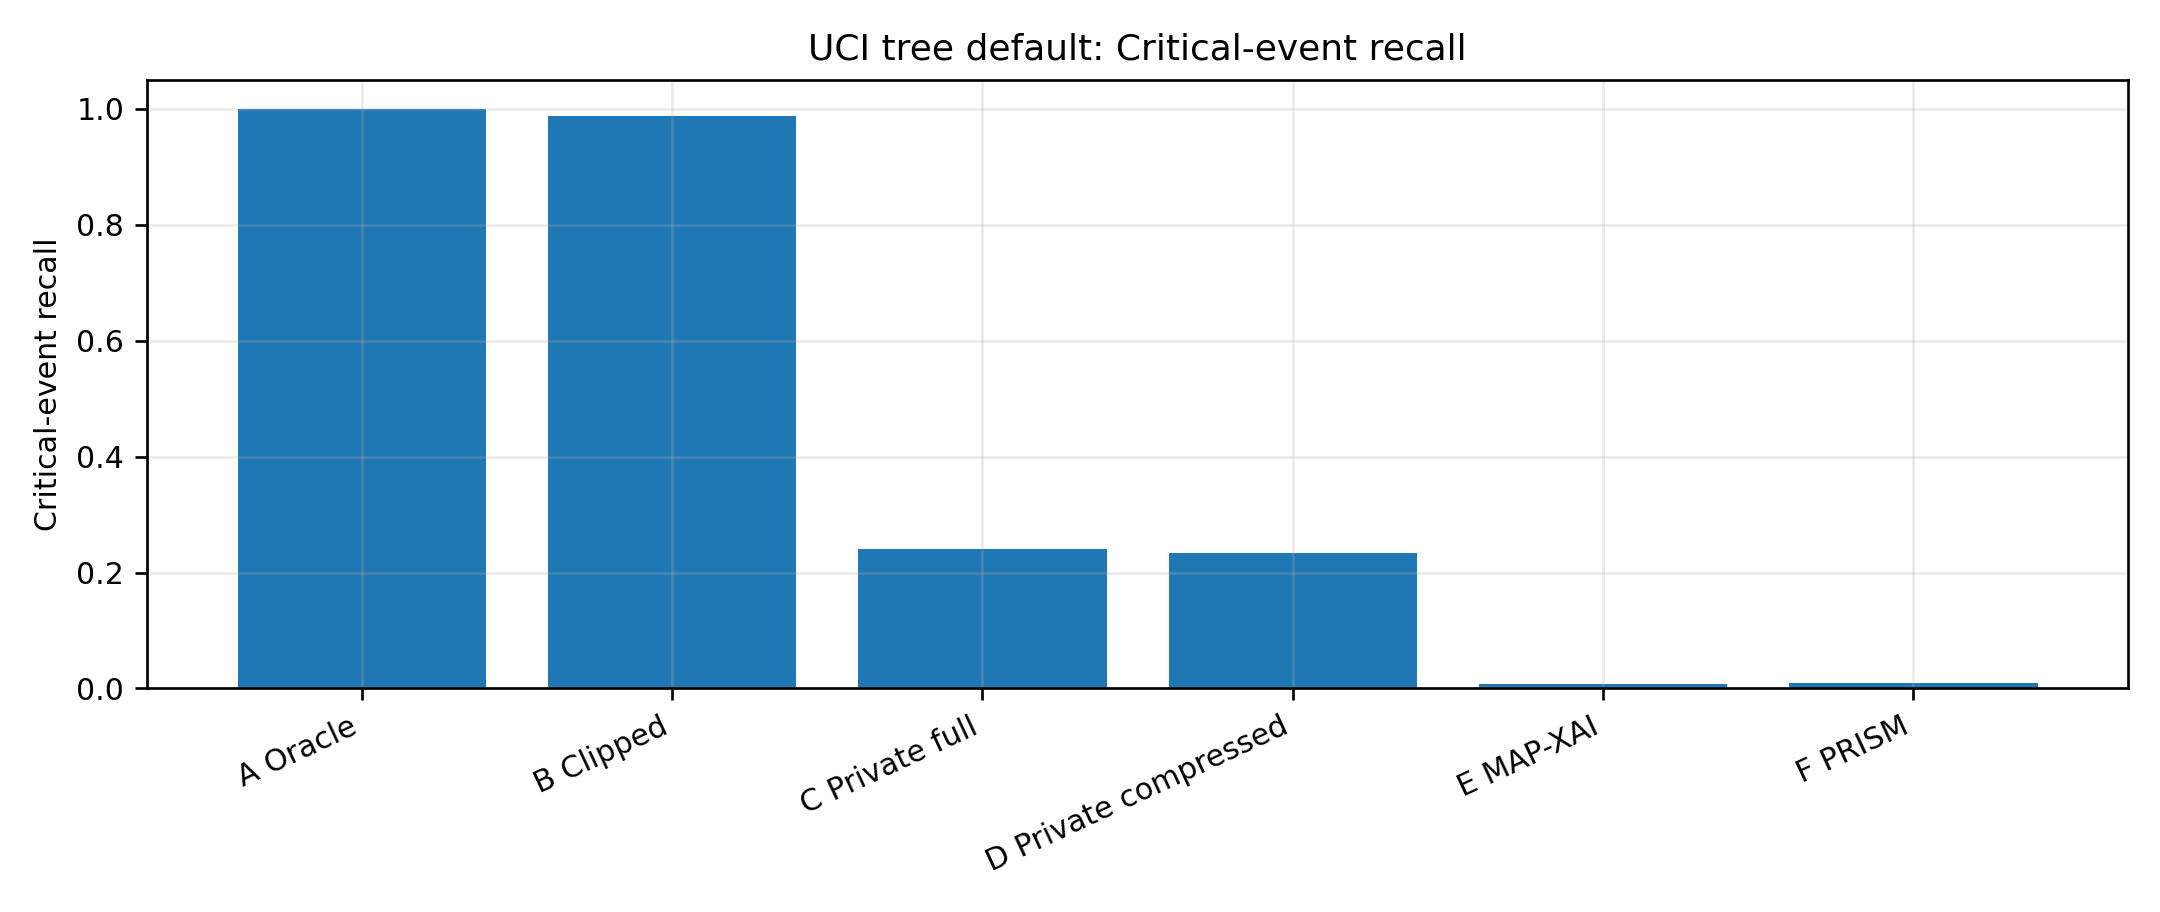
\includegraphics[width=\linewidth]{uci_tree_default_ladder_recall.png}\\[-1mm]
{\small (b) UCI recall}
\end{minipage}
\caption{Feasibility ladder for critical-event recall. The final MAP-XAI-only and PRISM-XAI stages reveal the additional service reduction introduced by sparse selective explanation delivery.}
\label{fig:ladder_recall}
\end{figure}

Figure~\ref{fig:ladder_recall} isolates the service-side effect: the strongest additional recall loss appears at Stages E--F, where selective scheduling reduces the number of explanation opportunities.

\subsection{Communication-Traffic Evidence}

\begin{figure}[htbp]
\centering
\begin{minipage}{.49\linewidth}
\centering
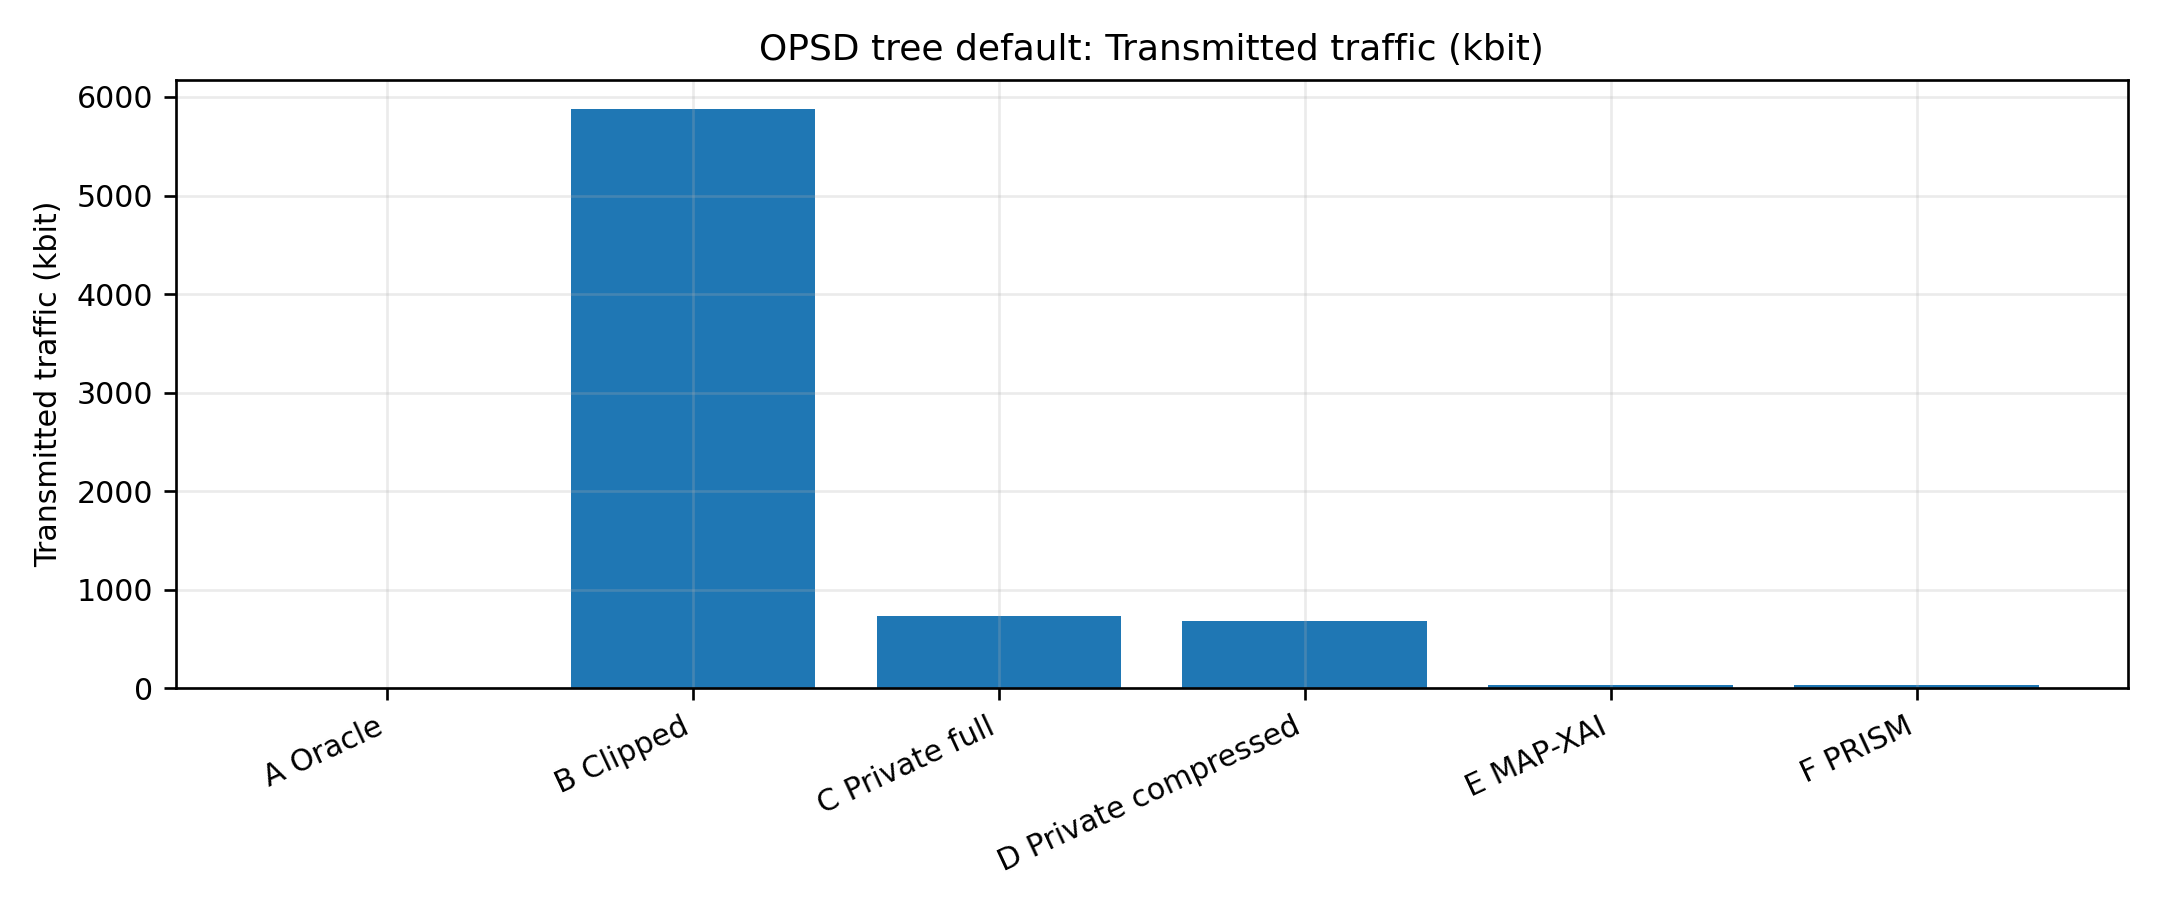
\includegraphics[width=\linewidth]{opsd_tree_default_ladder_traffic.png}\\[-1mm]
{\small (a) OPSD traffic}
\end{minipage}\hfill
\begin{minipage}{.49\linewidth}
\centering
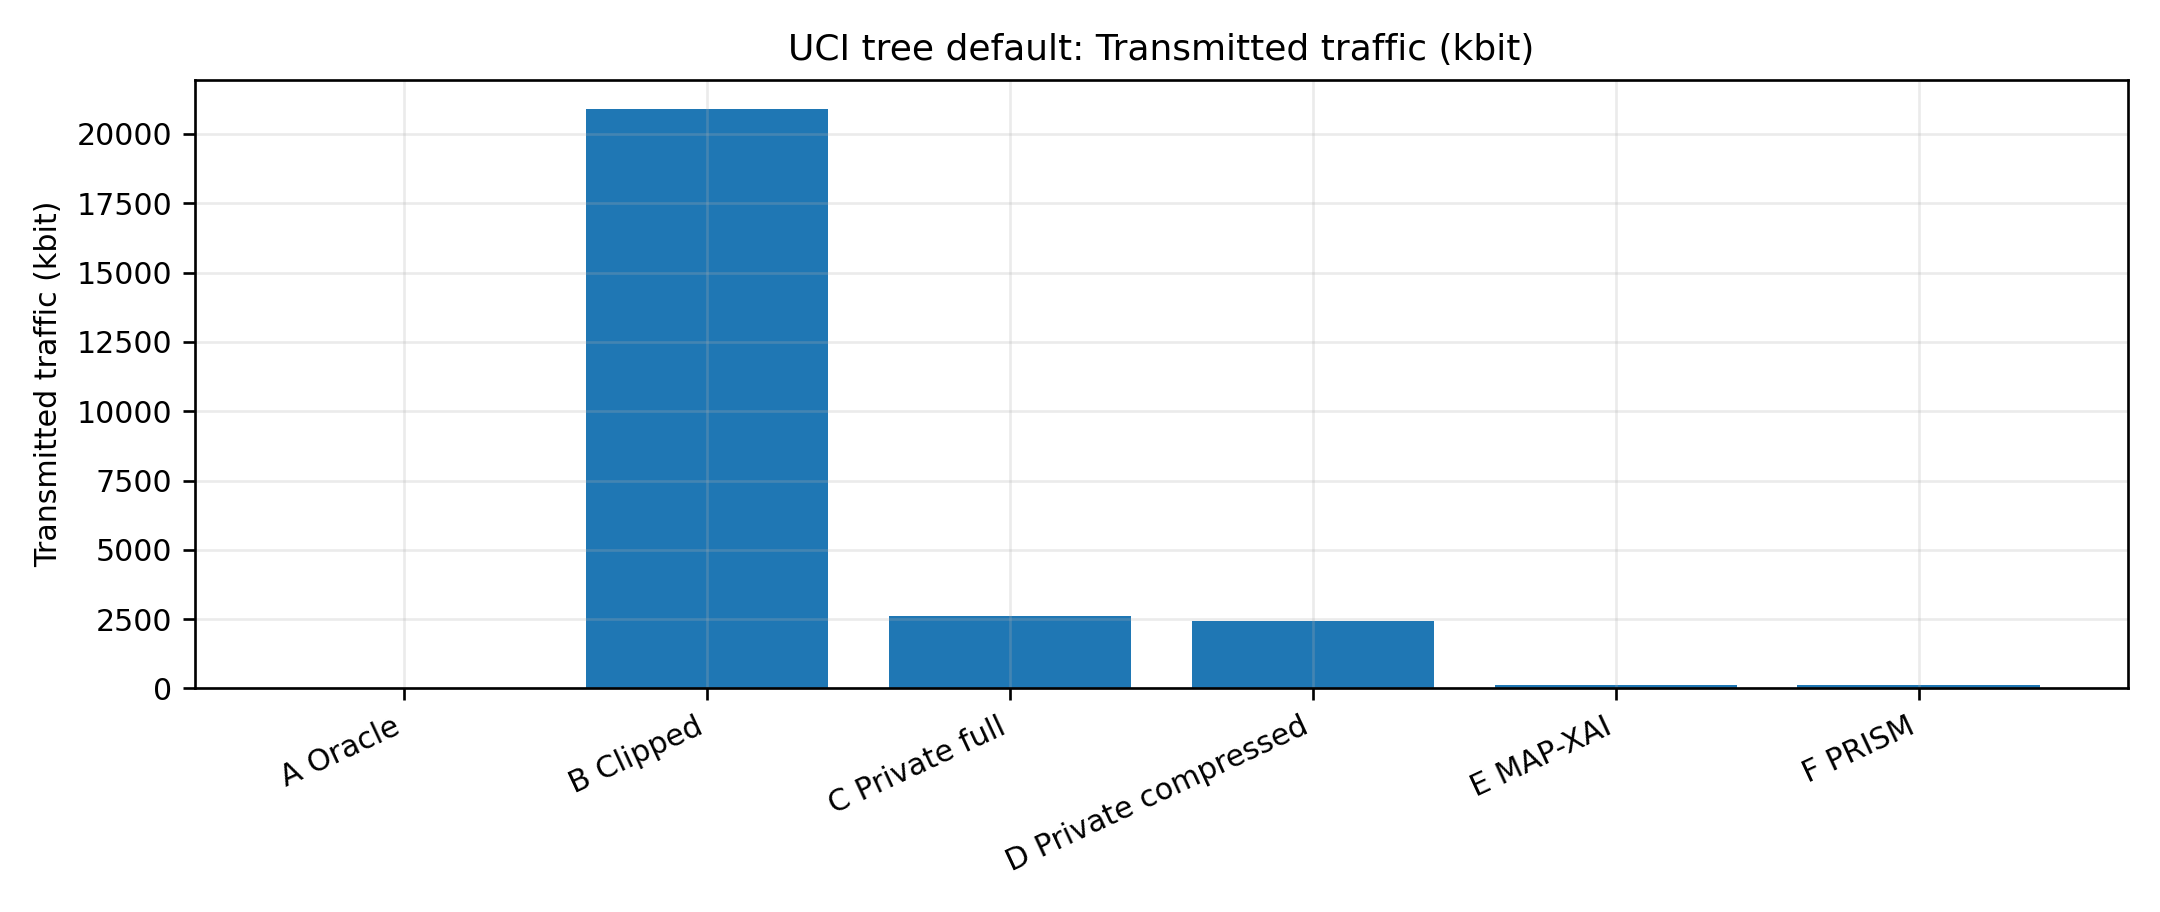
\includegraphics[width=\linewidth]{uci_tree_default_ladder_traffic.png}\\[-1mm]
{\small (b) UCI traffic}
\end{minipage}
\caption{Feasibility ladder for transmitted traffic. Post-DP semantic compression produces a modest reduction, whereas selective semantic release under MAP-XAI-only and PRISM-XAI produces the dominant communication saving.}
\label{fig:ladder_traffic}
\end{figure}

Figure~\ref{fig:ladder_traffic} provides the complementary communication diagnosis: compression reduces the size of an individual private packet, whereas the dominant traffic reduction occurs at Stages E--F by reducing the number of transmitted packets.

\subsection{Fidelity--Privacy Relationship}

\begin{figure}[htbp]
\centering
\begin{minipage}{.49\linewidth}
\centering
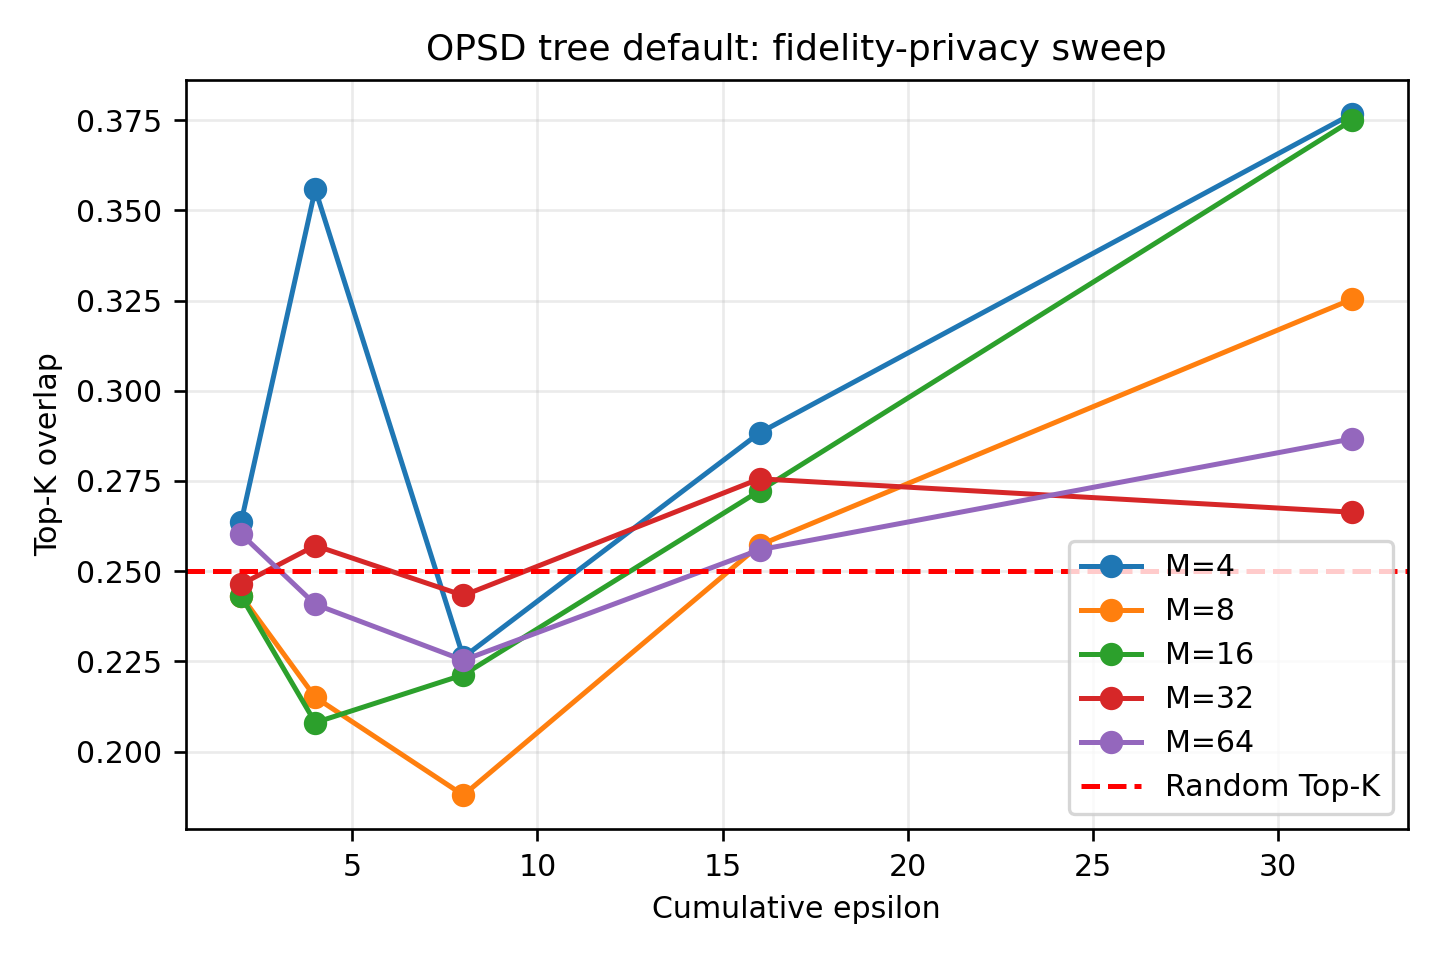
\includegraphics[width=\linewidth]{opsd_tree_default_fidelity_privacy_curve.png}\\[-1mm]
{\small (a) OPSD}
\end{minipage}\hfill
\begin{minipage}{.49\linewidth}
\centering
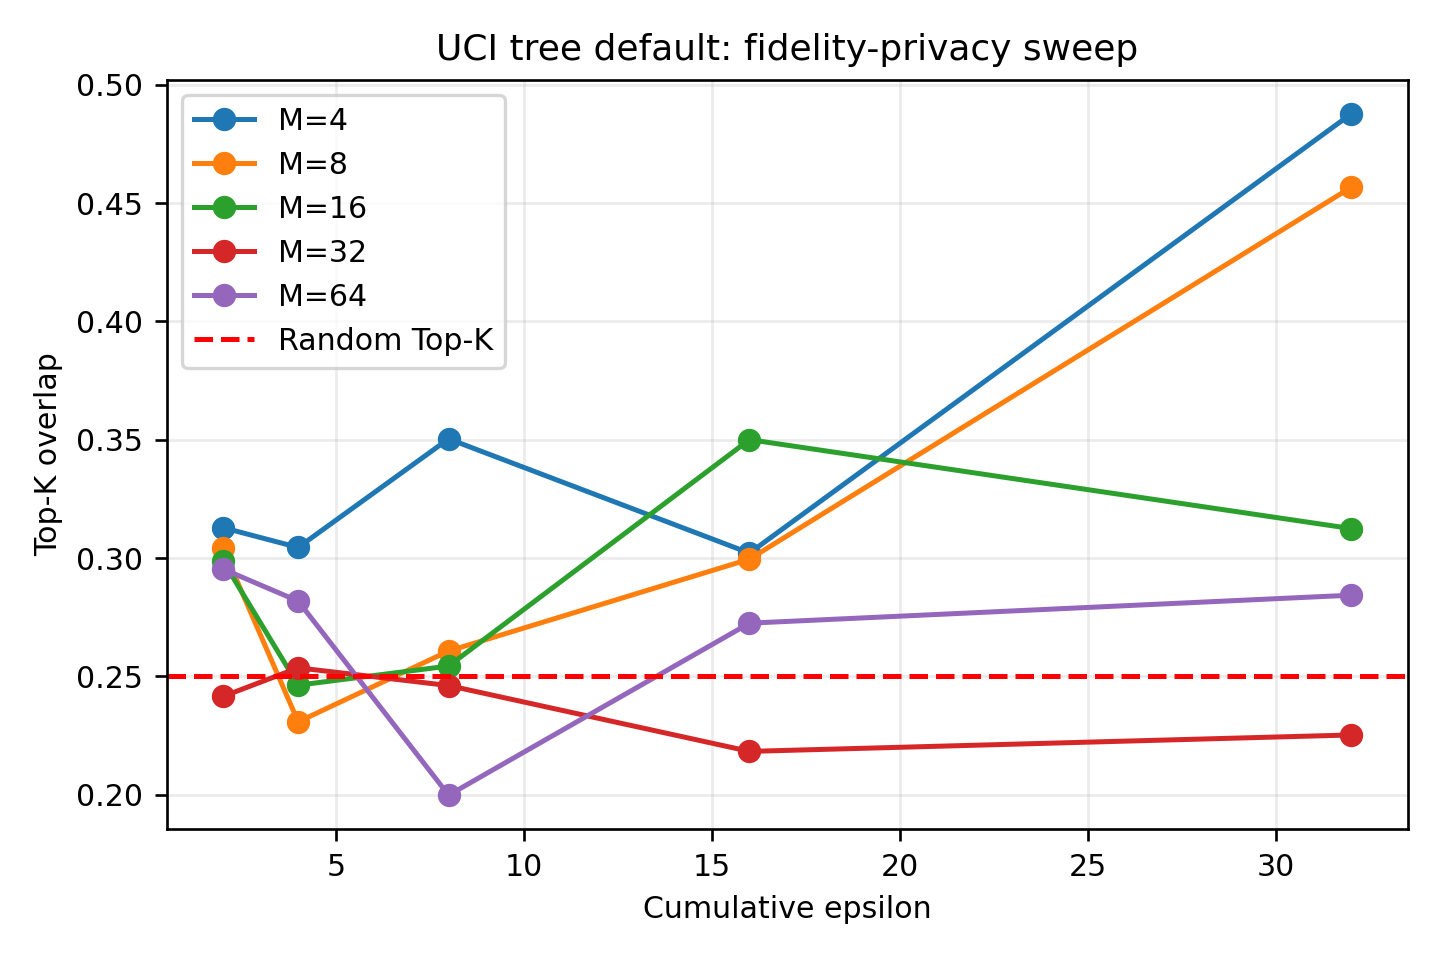
\includegraphics[width=\linewidth]{uci_tree_default_fidelity_privacy_curve.png}\\[-1mm]
{\small (b) UCI}
\end{minipage}
\caption{Diagnostic fidelity--privacy relationship. Increasing the cumulative privacy allowance can recover explanation fidelity, but the magnitude of the recovery is dataset dependent and requires greater household privacy expenditure.}
\label{fig:fidelity_privacy}
\end{figure}

The diagnosis of Stage C naturally raises the question of whether the privacy-induced fidelity loss can be reduced. Figure~\ref{fig:fidelity_privacy} shows that increasing the available privacy allowance can recover part of the explanation structure.

The recovery is nevertheless dataset dependent and is obtained by relaxing the cumulative household privacy guarantee. The privacy budget therefore represents a genuine fidelity--privacy trade-off rather than a scheduler hyperparameter that can be increased without consequence.

This result is consistent with the privacy-release sweep: explanation fidelity depends on both the total privacy allowance and the number of releases over which that allowance is composed.

\subsection{Recall--Traffic Relationship}

\begin{figure}[htbp]
\centering
\begin{minipage}{.49\linewidth}
\centering
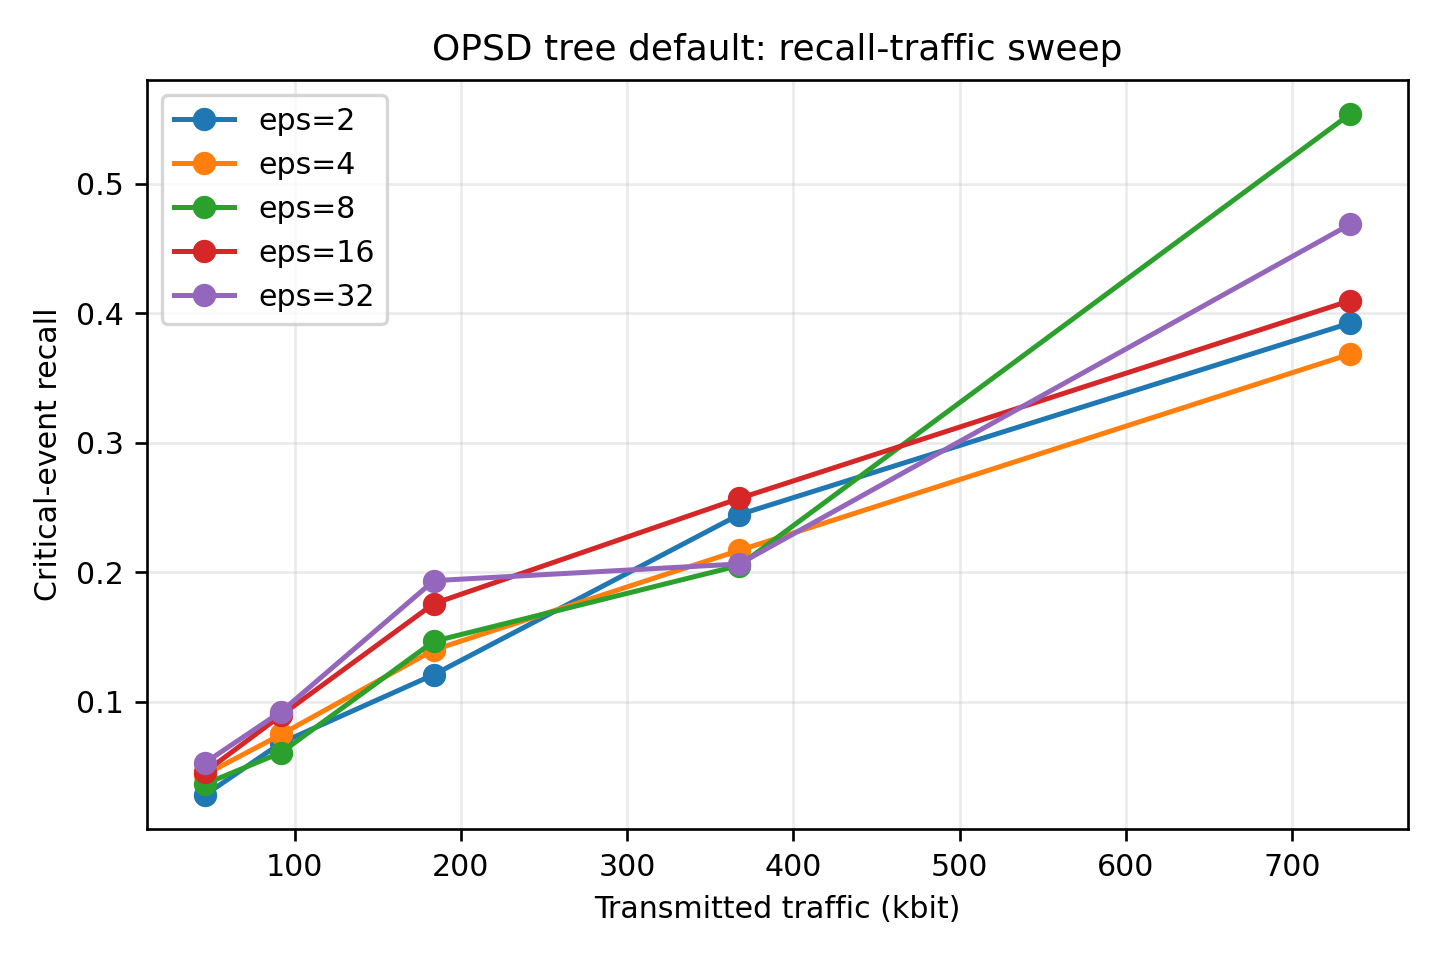
\includegraphics[width=\linewidth]{opsd_tree_default_recall_traffic_curve.png}\\[-1mm]
{\small (a) OPSD}
\end{minipage}\hfill
\begin{minipage}{.49\linewidth}
\centering
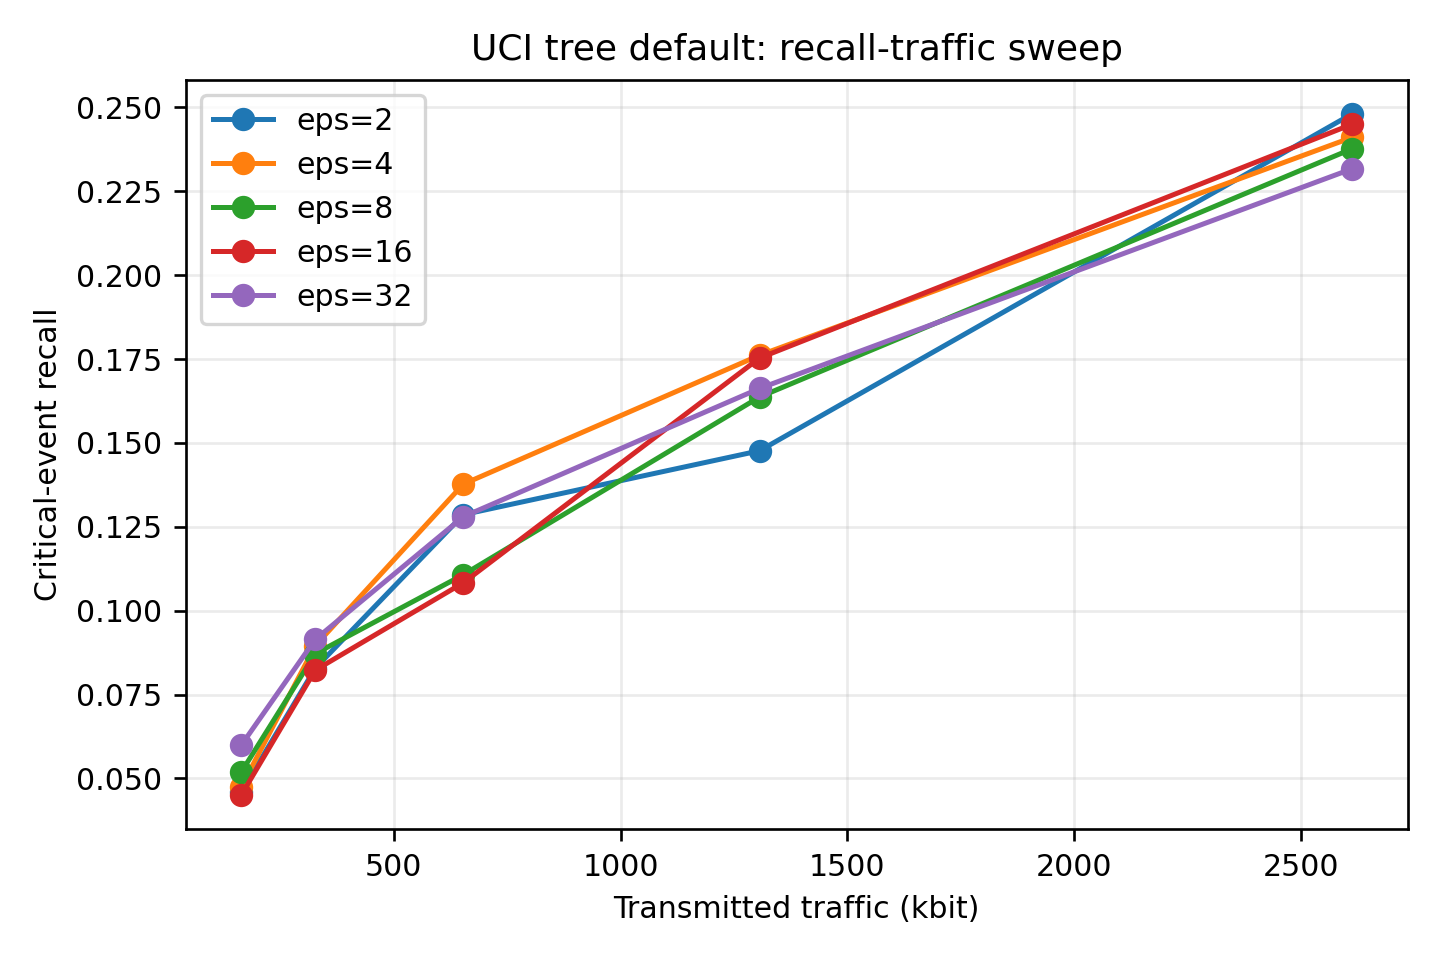
\includegraphics[width=\linewidth]{uci_tree_default_recall_traffic_curve.png}\\[-1mm]
{\small (b) UCI}
\end{minipage}
\caption{Diagnostic recall--traffic relationship. Higher critical-event recall is achievable by increasing the number of private explanation transmissions, but this requires substantially greater communication expenditure.}
\label{fig:recall_traffic}
\end{figure}

Figure~\ref{fig:recall_traffic} isolates the second major trade-off identified by the ladder. Critical-event recall can be increased by providing more explanation service, but the additional updates require considerably more private communication.

This confirms that the low recall of the most selective configurations is not an unexplained failure of the attribution representation. It is the operational consequence of choosing a low-traffic release regime.

\subsection{Mechanism-Level Interpretation}

Taken together, the feasibility ladder identifies two separate bottlenecks in the complete system.

The first occurs at the transition from the clipped explanation to the differentially private explanation. This stage causes the dominant reduction in Top-$K$ agreement and cosine similarity. The result identifies cumulative DP noise as the primary explanation-fidelity bottleneck.

The second occurs when the system moves from continuously available private packets to MAP-XAI/PRISM selective release. This stage produces the dominant reduction in communication traffic, but also reduces critical-event coverage and recall because many potential explanation transmissions are intentionally suppressed.

The complete causal interpretation is therefore

$$
\boxed{
\begin{array}{ll}
\text{Clipping} & \rightarrow \text{negligible fidelity loss},\\[1mm]
\text{Differential privacy} & \rightarrow \text{dominant fidelity loss},\\[1mm]
\text{Semantic compression} & \rightarrow \text{modest traffic reduction with little extra fidelity loss},\\[1mm]
\text{Selective scheduling} & \rightarrow \text{dominant traffic reduction and lower service coverage}.
\end{array}}
$$

This decomposition has direct implications for system improvement. Increasing scheduler complexity or retuning scheduling weights cannot recover attribution information already destroyed by the private mechanism. Improving explanation fidelity therefore requires attention to privacy allocation, release composition, sensitivity calibration, or the privacy horizon. In contrast, improving critical-event recall requires relaxing the selective-service regime, increasing the release cap, or otherwise allocating more transmission opportunities to critical periods.

The feasibility ladder therefore separates the two principal engineering questions of the proposed architecture: how much explanation information survives privacy protection, and how selectively the surviving information should be communicated.


\section{Privacy-Release Sweep: The Coverage--Fidelity--Privacy Frontier}\label{sec:privacy-release-frontier}

The main M8 evaluation fixes the maximum number of private releases at \(M=8\). This provides a consistent operating point for the statistical comparison, but it does not by itself show how the system changes when the release horizon is relaxed or tightened. The privacy-release sweep therefore varies both the cumulative privacy budget and the maximum number of private explanation releases,

$$
\epsilon_{\max}\in\{2,4,8,16,32\},
\qquad
M\in\{4,8,16,32,64\}.
$$

The experiment evaluates the resulting interaction among explanation-service frequency, communication traffic, critical-event coverage and recall, and explanation fidelity.

The two parameters control different but coupled aspects of the private explanation service. The release cap \(M\) determines the maximum number of private explanation updates that can be produced by an endpoint over the evaluation horizon. Increasing \(M\) therefore creates more opportunities to refresh the explanation and serve critical events. The cumulative privacy budget \(\epsilon_{\max}\), in contrast, determines the total privacy allowance available across those releases.

These quantities cannot be considered independently. Under a fixed horizon-level privacy budget, permitting more releases requires the privacy accountant to compose the guarantee over a larger number of private mechanisms. The corresponding Gaussian noise scale \(\sigma\) therefore increases as \(M\) increases at fixed \(\epsilon_{\max}\). Consequently, a larger release cap can improve service coverage while simultaneously degrading the fidelity of each individual private explanation.

This interaction creates a three-way frontier:

$$
\text{more releases}
\;\Longrightarrow\;
\text{higher service opportunity and traffic},
$$

but, under fixed cumulative privacy,

$$
\text{more releases}
\;\Longrightarrow\;
\text{stronger per-release perturbation},
$$

which can reduce explanation fidelity. The resulting operating point is therefore determined jointly by \(M\) and \(\epsilon_{\max}\), rather than by either parameter alone.

\subsection{Coverage and Recall Increase with the Release Horizon}

The most consistent effect of increasing \(M\) is an increase in service coverage. A larger release cap provides additional opportunities for the scheduler to deliver explanations during critical operating periods.

The \(\epsilon_{\max}=32\) OPSD frontier provides a clear example. With \(M=4\), the system achieves \(8.4\%\) critical-event coverage and \(5.3\%\) critical-event recall while transmitting \(45.9\) kbit. Increasing the release cap to \(M=16\) raises coverage to \(31.1\%\) and recall to \(19.4\%\), with traffic increasing to \(183.7\) kbit. At \(M=64\), coverage reaches \(83.0\%\) and recall reaches \(46.9\%\), while traffic increases to \(735.0\) kbit.

Thus,

$$
\begin{array}{c|ccc}
M & 4 & 16 & 64\\
\hline
\text{Critical coverage} & 0.084 & 0.311 & 0.830\\
\text{Critical recall} & 0.053 & 0.194 & 0.469\\
\text{Traffic (kbit)} & 45.9 & 183.7 & 735.0
\end{array}
$$

shows the direct service--communication trade-off. Increasing the release horizon substantially improves the probability that a critical event receives a fresh explanation, but the communication requirement rises correspondingly.

The same trend appears on UCI. At \(\epsilon_{\max}=32\), \(M=4\) provides approximately \(10.3\%\) critical-event coverage, whereas \(M=64\) increases coverage to approximately \(53.5\%\). The communication cost rises much more strongly, from approximately \(163.3\) kbit to \(2613.2\) kbit.

The release cap is therefore an effective mechanism for controlling service intensity. Larger values of \(M\) move the system toward higher explanation availability, while smaller values move it toward strongly selective private explanation delivery.

\subsection{Explanation Fidelity Is Non-Monotone in the Number of Releases}

The explanation-fidelity behavior is fundamentally different from the coverage behavior. Increasing the number of permitted releases does not monotonically improve Top-\(K\) agreement or cosine similarity.

For OPSD at \(\epsilon_{\max}=32\), Top-\(K\) agreement is \(0.377\) at \(M=4\), \(0.375\) at \(M=16\), and \(0.287\) at \(M=64\). Thus, increasing the release cap from \(4\) to \(64\) increases critical-event coverage by nearly an order of magnitude, from \(8.4\%\) to \(83.0\%\), while Top-\(K\) agreement decreases from \(0.377\) to \(0.287\).

The corresponding UCI effect is even clearer. At the same privacy budget,

$$
M=4:
\qquad
\text{coverage}=0.103,
\qquad
\text{Top-}K=0.488,
$$

whereas

$$
M=64:
\qquad
\text{coverage}=0.535,
\qquad
\text{Top-}K=0.284.
$$

Traffic simultaneously increases from \(163.3\) kbit to \(2613.2\) kbit.

The reduction in fidelity is consistent with the cumulative privacy mechanism. A fixed horizon-level privacy allowance must support an increasing number of potential releases. The associated increase in per-release Gaussian perturbation can therefore remove more of the attribution structure from each transmitted explanation.

Consequently,

$$
M\uparrow
\quad\Longrightarrow\quad
\text{coverage generally}\uparrow,
$$

does not imply

$$
M\uparrow
\quad\Longrightarrow\quad
\text{fidelity}\uparrow.
$$

Instead, service coverage and private-explanation fidelity move along different dimensions of the operating frontier.

\subsection{Role of the Cumulative Privacy Budget}

Varying \(\epsilon_{\max}\) exposes the complementary part of this interaction. At fixed \(M\), increasing the cumulative privacy allowance permits a smaller Gaussian noise scale and can preserve more of the original explanation structure.

This effect is particularly visible for small release caps. For example, UCI with \(M=4\) reaches Top-\(K\) agreement of \(0.488\) at \(\epsilon_{\max}=32\). The larger privacy allowance permits substantially greater fidelity than can be obtained when the same release cap operates under a much tighter cumulative privacy constraint.

The improvement is not without cost. Increasing \(\epsilon_{\max}\) explicitly relaxes the household-level privacy guarantee. The privacy budget therefore cannot be increased solely to optimize explanation fidelity without changing the privacy protection offered by the system.

The sweep consequently exposes two distinct mechanisms:

$$
M:
\quad
\text{controls how frequently private explanations may be released},
$$

and

$$
\epsilon_{\max}:
\quad
\text{controls how much cumulative privacy loss is permitted}.
$$

Their interaction determines the per-release noise level and therefore the amount of explanation information that survives the private mechanism.

\subsection{Dataset Dependence of the Frontier}

The OPSD and UCI surfaces show that the privacy-release frontier is also dataset dependent.

OPSD can recover relatively high critical-event coverage as \(M\) increases. At \(\epsilon_{\max}=32\) and \(M=64\), coverage reaches \(83.0\%\). Under the same \((\epsilon_{\max},M)\) setting, UCI reaches \(53.5\%\).

The communication requirements are also substantially different. The \(M=64,\epsilon_{\max}=32\) operating point requires approximately \(735.0\) kbit on OPSD but approximately \(2613.2\) kbit on UCI.

Explanation fidelity exhibits an additional difference. OPSD retains comparatively stronger Top-\(K\) structure at several high-budget operating points, whereas UCI exhibits a stronger decline as the release horizon expands. This is consistent with the broader v19 evidence, in which UCI remains more difficult under cumulative private explanation release even when communication resources are available.

The same nominal values of \(M\) and \(\epsilon_{\max}\) therefore do not imply the same service or fidelity outcome across datasets.

\subsection{Connection to the M8 and M4 Operating Points}

The sweep provides additional context for the \(M=8\) configuration used in the main statistical experiment.

M8 does not maximize critical-event coverage. Larger release caps clearly provide greater service frequency. Instead, M8 selects a region in which private explanation transmission remains strongly selective relative to the 512-slot evaluation horizon.

For OPSD at \(\epsilon_{\max}=32\), increasing \(M\) from \(8\) to \(64\) raises coverage from approximately \(15.8\%\) to \(83.0\%\), but traffic increases from approximately \(91.9\) kbit to \(735.0\) kbit. On UCI, the same change raises coverage from approximately \(18.2\%\) to \(53.5\%\), while traffic increases from approximately \(326.7\) kbit to \(2613.2\) kbit.

The M4 sensitivity experiment moves in the opposite direction. Reducing the release cap from \(M=8\) to \(M=4\) lowers communication further, but the resulting service becomes sufficiently selective that the configured critical-event coverage floor is violated in most M4 PRISM runs. M8 therefore represents a more defensible selective-service operating point for the main comparison, while the wider release sweep demonstrates the alternative coverage--traffic regimes available at larger \(M\).

\subsection{Implications for Privacy-Aware Scheduling}

The privacy-release sweep demonstrates that the principal design problem is not simply explanation compression or scheduler-weight selection. The scheduler operates under a finite privacy horizon whose allocation directly affects both the frequency and the fidelity of private explanations.

Increasing the number of releases can improve critical-event service, but it also increases communication and can force stronger perturbation of each individual explanation. Increasing the privacy allowance can reduce this perturbation, but only by accepting greater cumulative privacy expenditure.

The resulting design objective is therefore to allocate a finite privacy allowance over time according to the operational value of explanation updates. Selective release is useful not only because it saves transmitted bits, but also because avoiding low-value private releases preserves privacy resources for later conditions in which a new explanation may be more important.

This result also establishes a limitation of scheduler optimization. Once attribution information has been strongly degraded by the private mechanism, subsequent scheduling cannot reconstruct the removed explanation structure. Scheduler adaptation can determine \emph{when} privacy should be spent and \emph{which} available packet should be transmitted, but it cannot recover fidelity that has already been lost through excessive privacy perturbation.

The joint privacy-horizon and release policy is therefore a fundamental system-design variable. The appropriate operating point depends on the required critical-event service level, the acceptable communication load, the desired explanation fidelity, and the household-level privacy guarantee.

\begin{figure}[htbp]
\centering
\begin{minipage}{.49\linewidth}
\centering
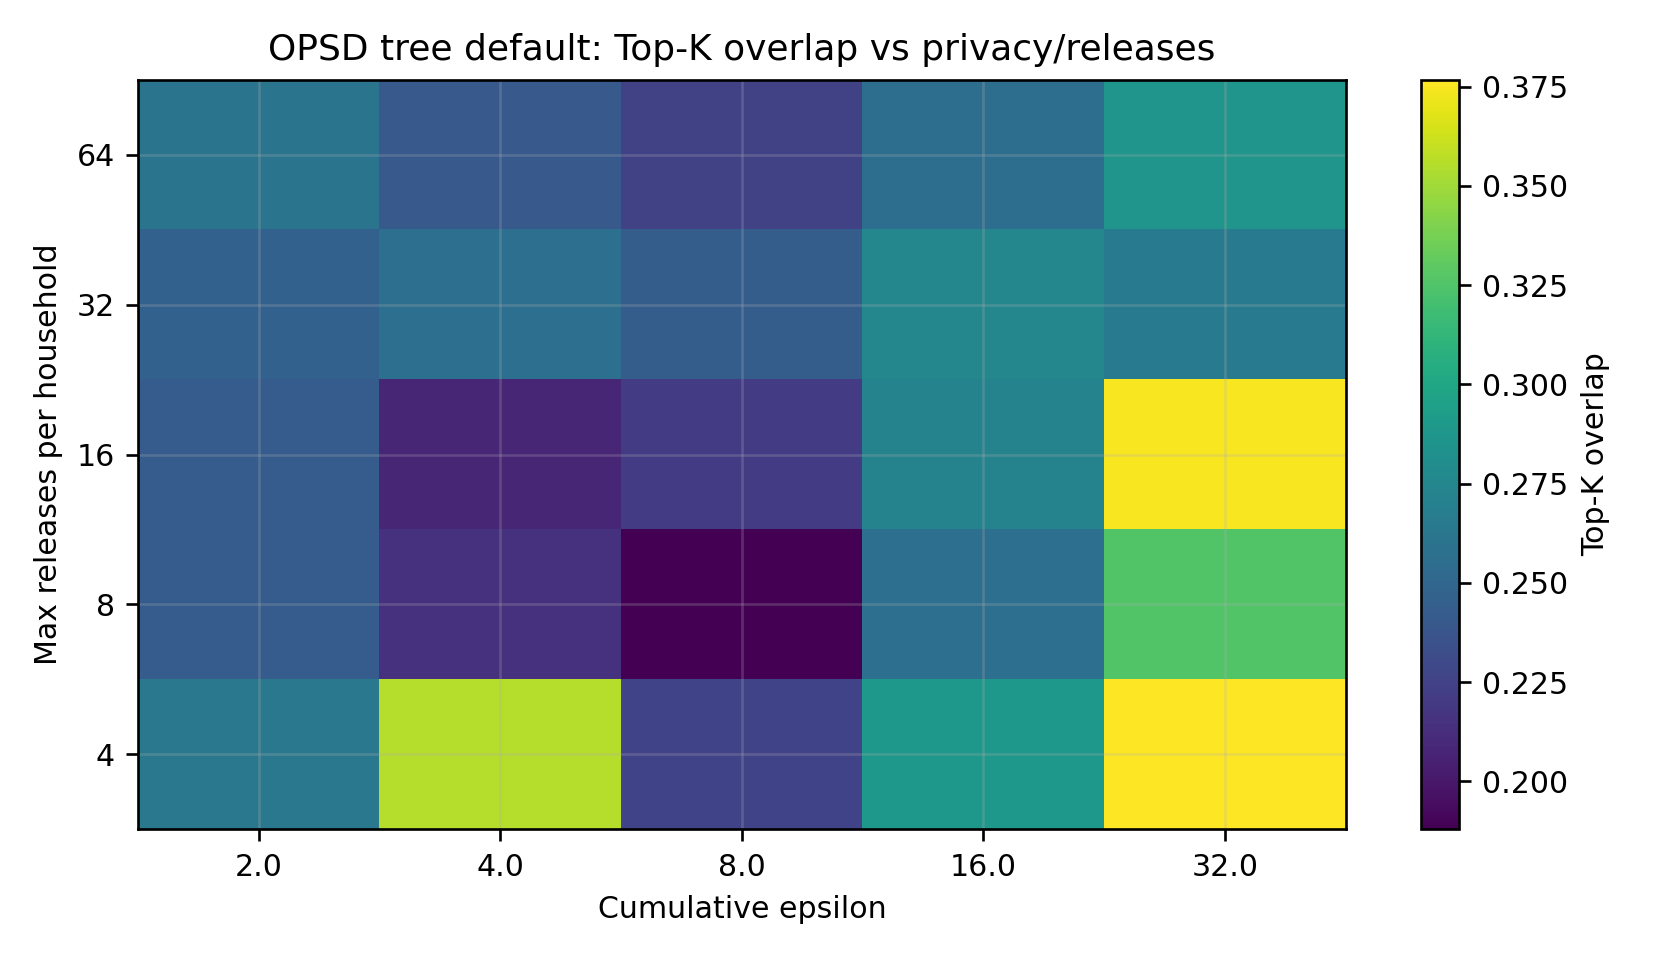
\includegraphics[width=\linewidth]{opsd_tree_default_privacy_sweep_topk_overlap.png}\\[-1mm]
{\small (a) OPSD Top-$K$}
\end{minipage}\hfill
\begin{minipage}{.49\linewidth}
\centering
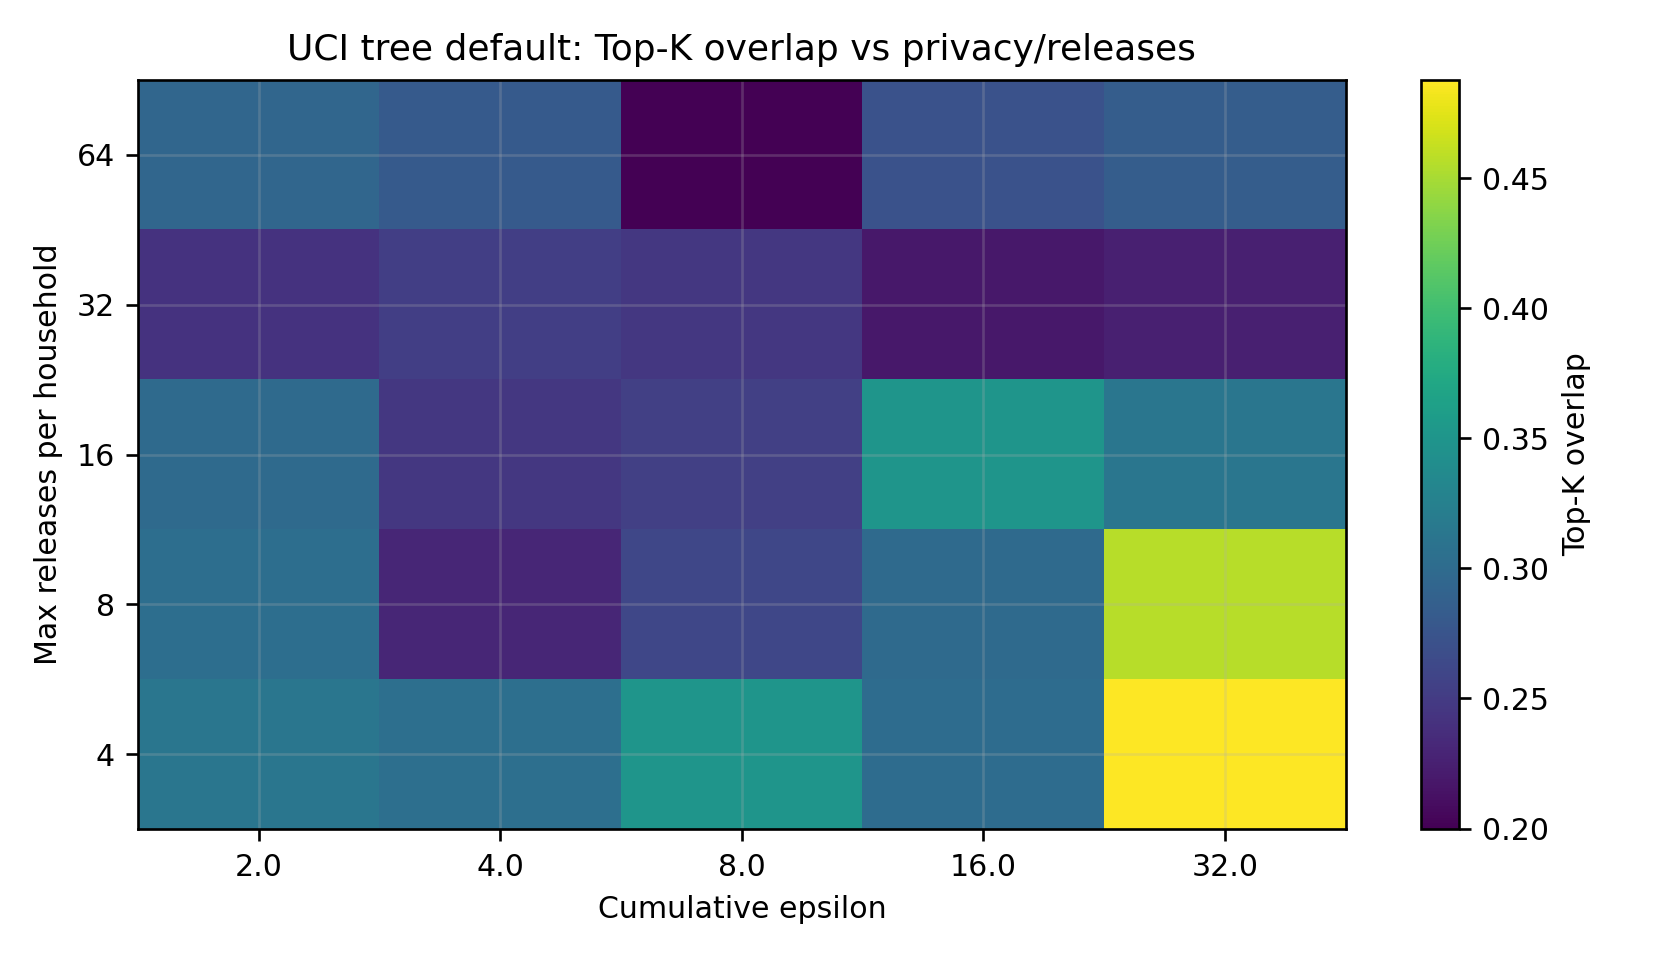
\includegraphics[width=\linewidth]{uci_tree_default_privacy_sweep_topk_overlap.png}\\[-1mm]
{\small (b) UCI Top-$K$}
\end{minipage}
\caption{Privacy-release sweep for Top-$K$ agreement. Increasing the release cap \(M\) does not monotonically improve explanation fidelity because the fixed horizon-level privacy allowance must be composed across a larger number of potential releases.}
\label{fig:sweep_topk}
\end{figure}

Figure~\ref{fig:sweep_topk} shows the resulting Top-$K$ surfaces. The non-monotone variation across \(M\) distinguishes explanation fidelity from service coverage: additional transmission opportunities do not necessarily preserve the dominant attribution ranking when stronger per-release privacy perturbation is required.

\begin{figure}[htbp]
\centering
\begin{minipage}{.49\linewidth}
\centering
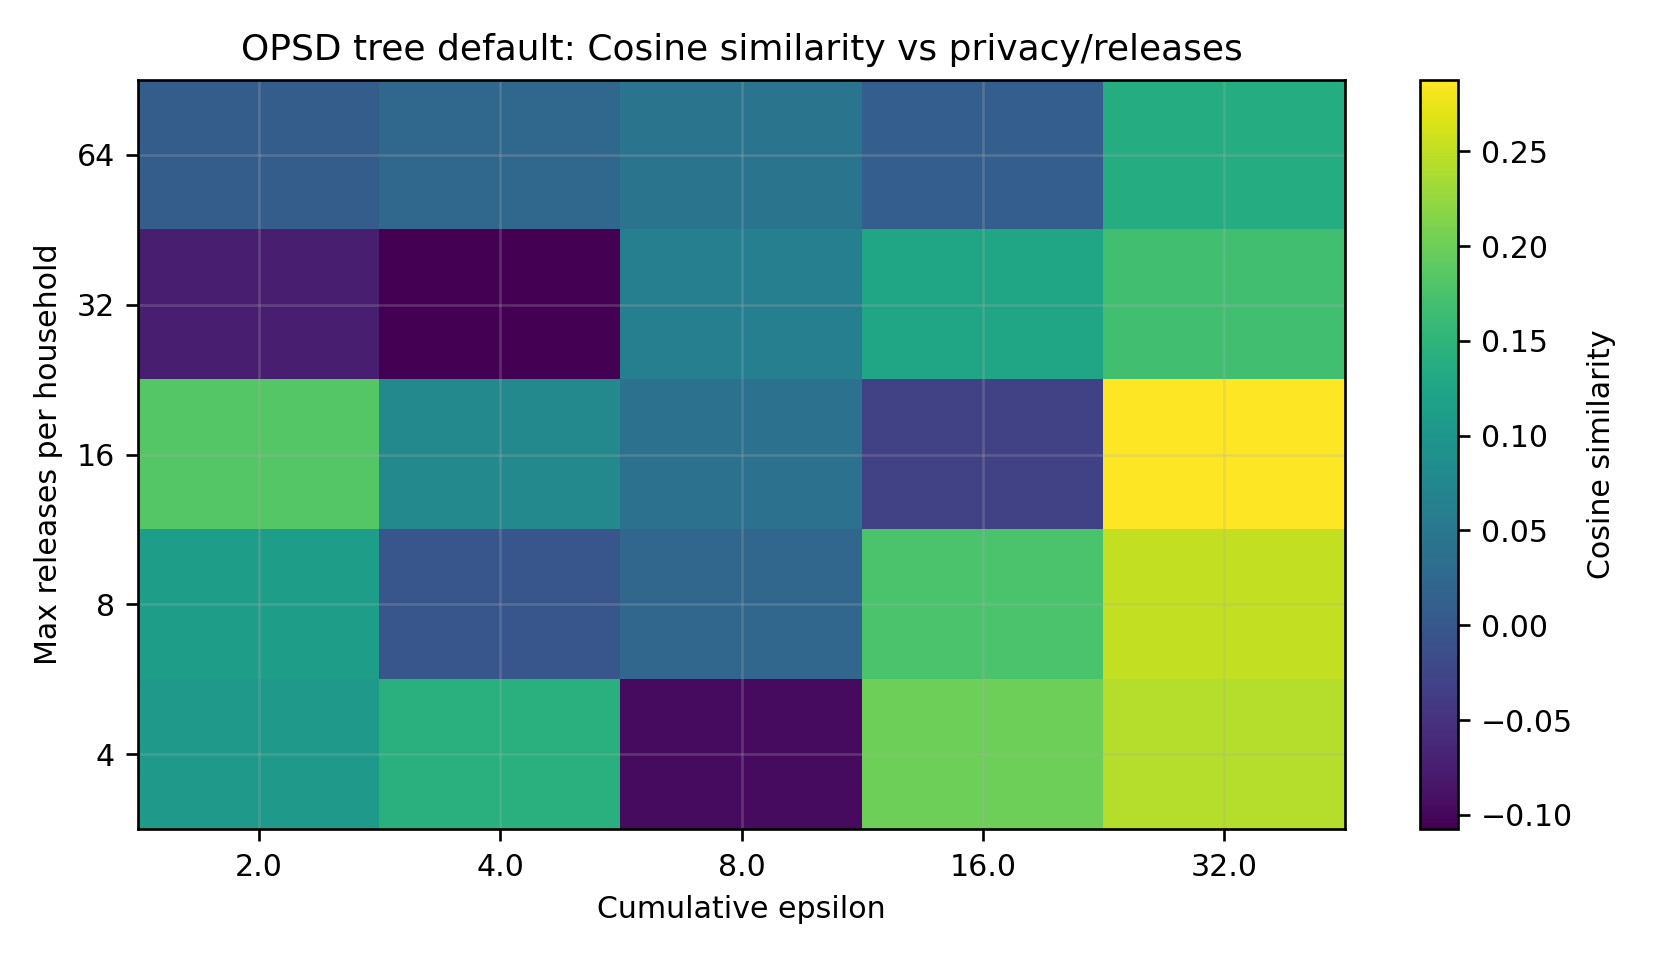
\includegraphics[width=\linewidth]{opsd_tree_default_privacy_sweep_cosine_similarity.png}\\[-1mm]
{\small (a) OPSD cosine}
\end{minipage}\hfill
\begin{minipage}{.49\linewidth}
\centering
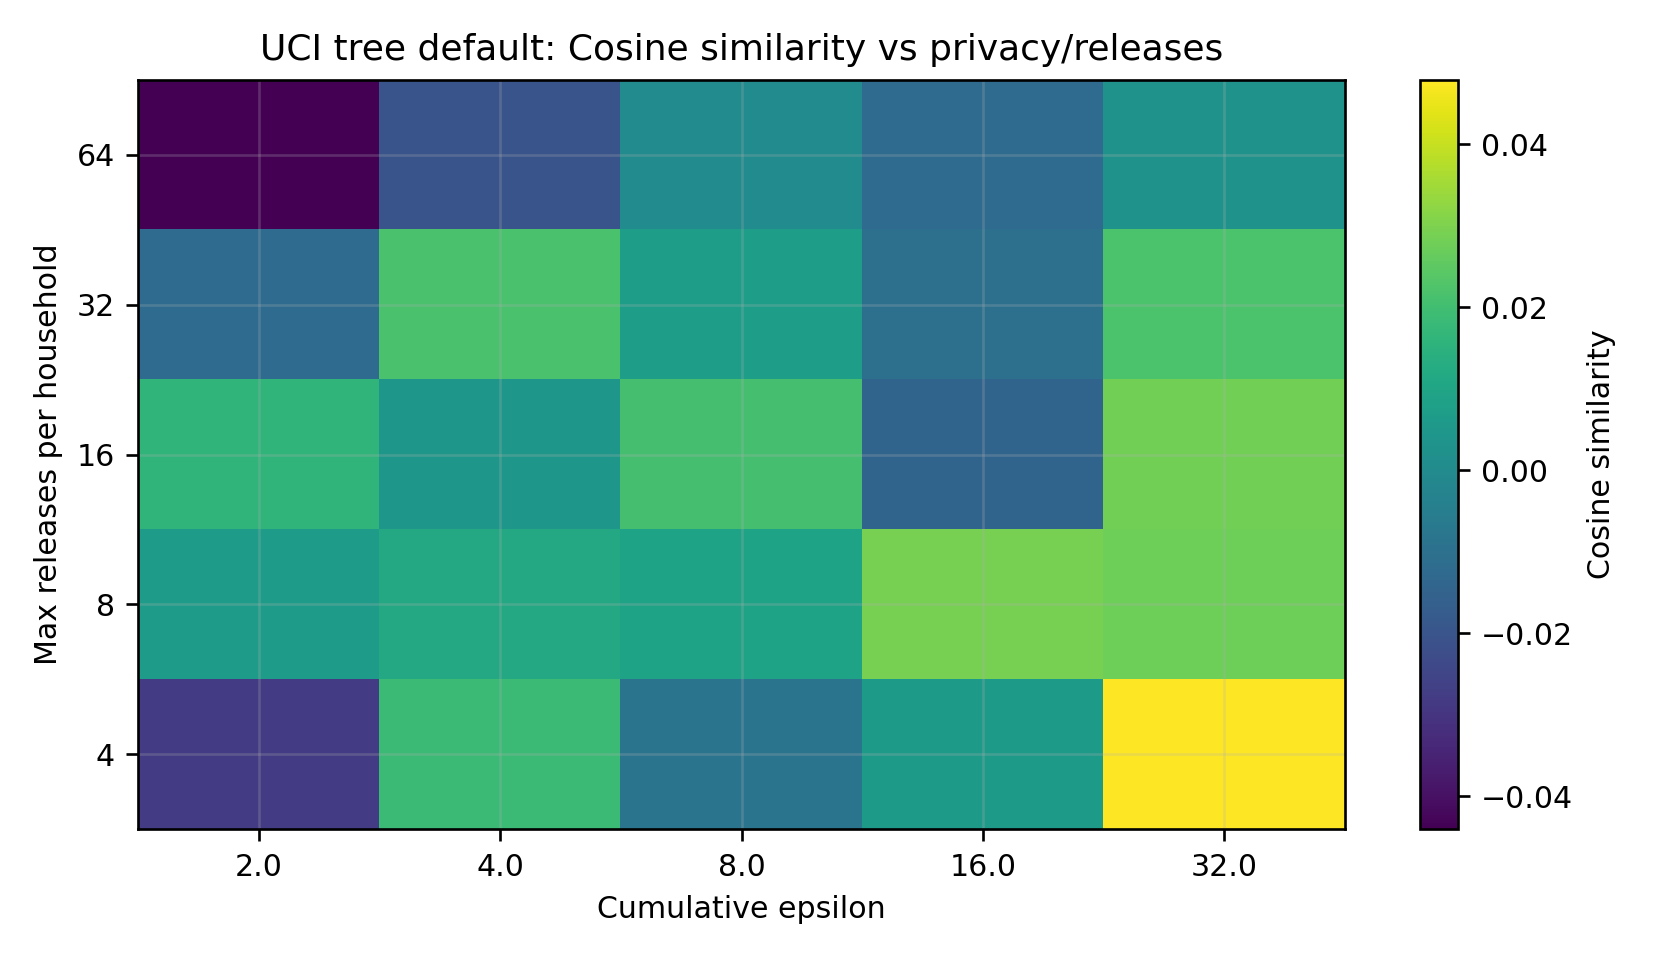
\includegraphics[width=\linewidth]{uci_tree_default_privacy_sweep_cosine_similarity.png}\\[-1mm]
{\small (b) UCI cosine}
\end{minipage}
\caption{Privacy-release sweep for cosine similarity. The irregular fidelity surface reflects the joint influence of cumulative privacy allowance, release horizon, and dataset-specific explanation structure.}
\label{fig:sweep_cosine}
\end{figure}

The cosine-similarity results in Fig.~\ref{fig:sweep_cosine} reinforce the same conclusion using the complete attribution direction rather than only the overlap of the dominant features. The surface is not ordered monotonically by the number of permitted releases, confirming that explanation quality depends on the privacy composition associated with those releases.

\begin{figure}[htbp]
\centering
\begin{minipage}{.49\linewidth}
\centering
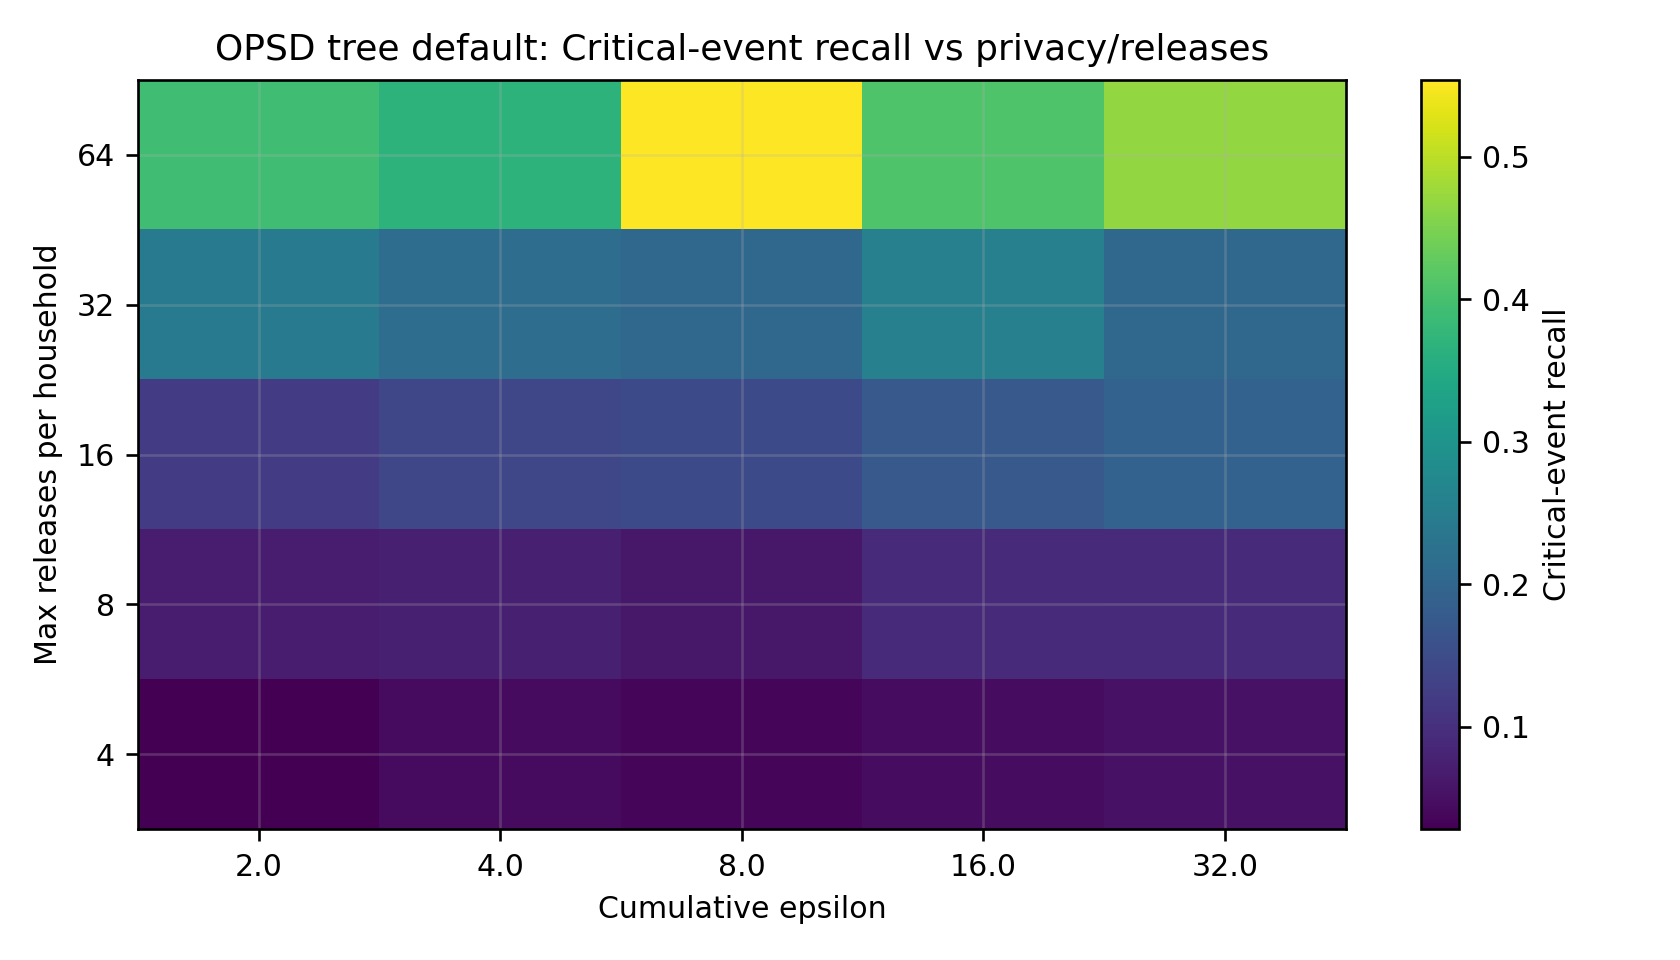
\includegraphics[width=\linewidth]{opsd_tree_default_privacy_sweep_critical_event_recall.png}\\[-1mm]
{\small (a) OPSD recall}
\end{minipage}\hfill
\begin{minipage}{.49\linewidth}
\centering
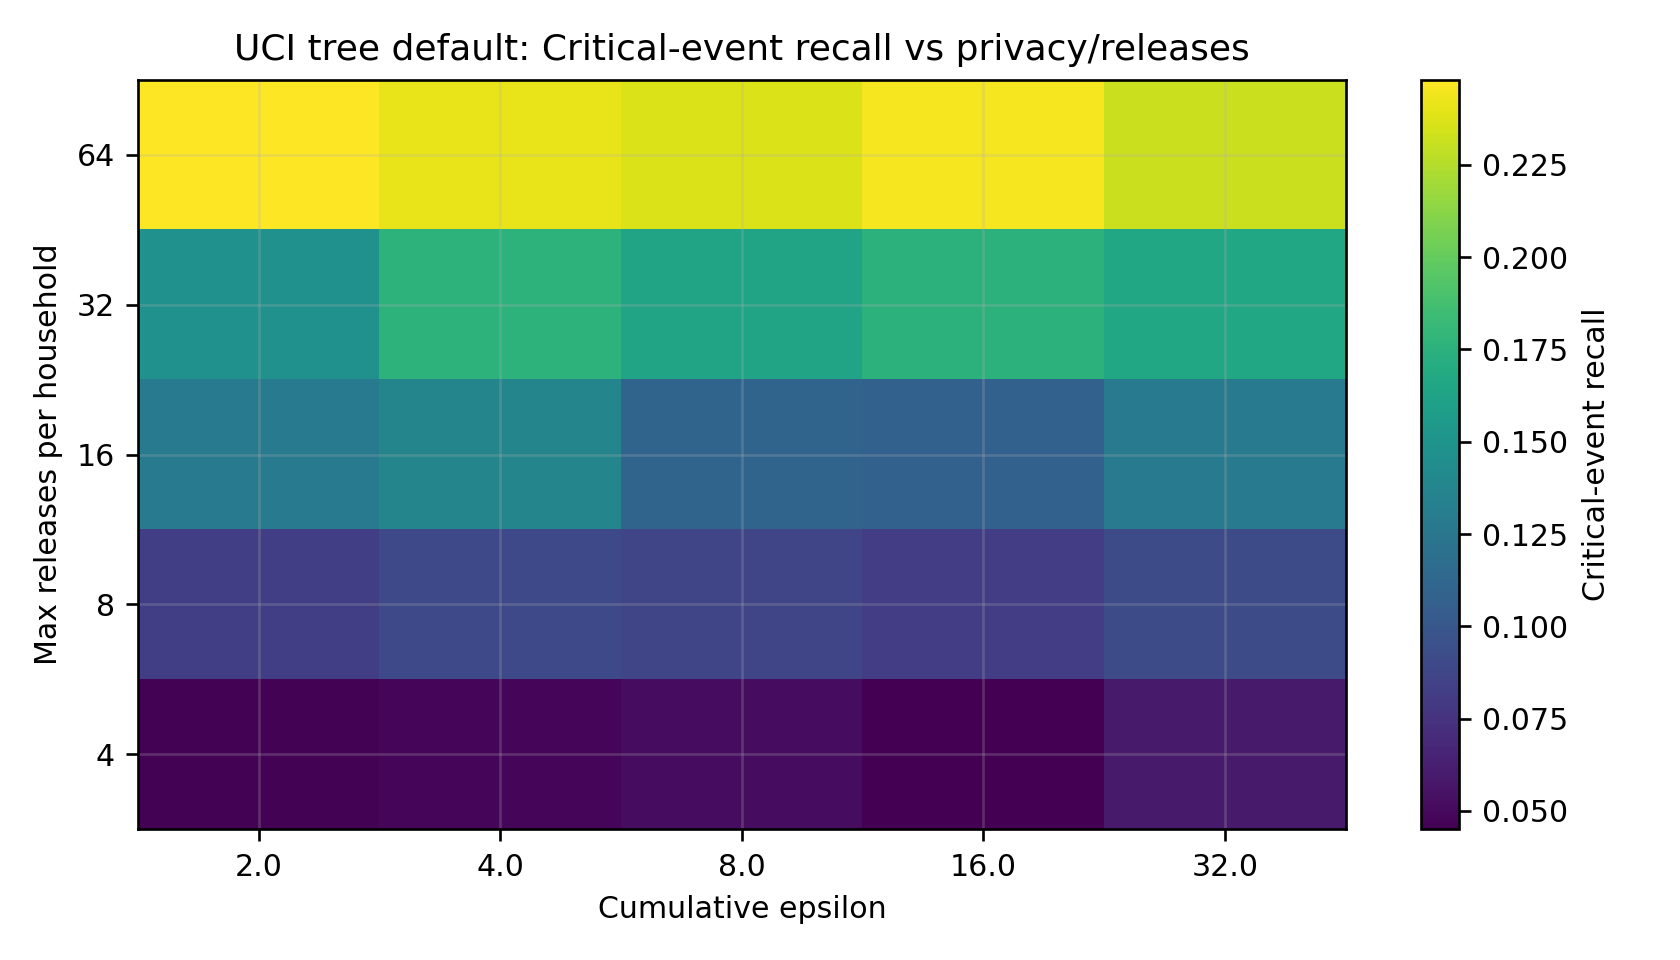
\includegraphics[width=\linewidth]{uci_tree_default_privacy_sweep_critical_event_recall.png}\\[-1mm]
{\small (b) UCI recall}
\end{minipage}
\caption{Privacy-release sweep for critical-event recall. In contrast to explanation fidelity, recall generally increases as additional private-release opportunities become available, exposing the central service--fidelity trade-off.}
\label{fig:sweep_recall}
\end{figure}

Figure~\ref{fig:sweep_recall} provides the complementary operational view. Critical-event recall generally increases with \(M\), whereas the Top-$K$ and cosine surfaces remain non-monotone. Taken together, the three sweep figures demonstrate that increasing the private-release horizon primarily expands service opportunities; it does not guarantee that the additional private explanations retain higher fidelity.

\part{Complete Metric-Family Analysis}
\section{Metric-by-metric macro tables}
The following four tables expose every quantitative family in the 720-row M8 result file. They are interpreted as a joint scorecard rather than as four independent leaderboards.

\subsection{Explanation-quality metrics}
Table~\ref{tab:macroexp} shows that exact Top-$K$ remains close to the 0.25 random reference, while the proposed modes recover more cosine, Spearman, and sign structure and much lower hierarchical distortion. High collapse rates remain, so the explanations are not uniformly faithful; the attack AUC is reported separately and is not used as the formal privacy guarantee.
% In the preamble:
% \usepackage{adjustbox}
% \usepackage{booktabs}

\begin{table*}[t]
\centering
\caption{Macro-average explanation-quality metrics over all v19 M8 conditions.}
\label{tab:macroexp}
\scriptsize
\setlength{\tabcolsep}{3pt}
\renewcommand{\arraystretch}{1.08}

\begin{adjustbox}{max width=\textwidth}
\begin{tabular}{lrrrrrrrrr}
\toprule
Method
& Cosine
& Spearman
& Top-K
& Sign agr.
& Hier. dist.
& Collapse
& Max collapse
& Attack AUC
& Rand. Top-K \\
\midrule

Periodic fixed-DP
& -0.003 & -0.015 & 0.252 & 0.502
& 263.0 & 1.000 & 505.2 & 0.690 & 0.250 \\

Channel fixed-DP
& -0.005 & 0.001 & 0.264 & 0.505
& 241.2 & 0.999 & 506.7 & 0.670 & 0.250 \\

AoX fixed-DP
& -0.007 & -0.015 & 0.255 & 0.500
& 263.2 & 1.000 & 510.1 & 0.664 & 0.250 \\

Joint full packet
& -0.005 & -0.002 & 0.260 & 0.510
& 131.1 & 1.000 & 506.1 & 0.661 & 0.250 \\

\midrule

MAP-XAI-only (ours)
& \textbf{0.119}
& \textbf{0.084}
& 0.265
& \textbf{0.573}
& \textbf{11.17}
& 0.961
& \textbf{434.3}
& 0.712
& 0.250 \\

PRISM-XAI (ours)
& 0.105
& 0.072
& \textbf{0.279}
& 0.565
& 12.07
& \textbf{0.954}
& 435.9
& 0.711
& 0.250 \\

\bottomrule
\end{tabular}
\end{adjustbox}
\end{table*}

\subsection{Operational metrics}
Table~\ref{tab:macroop} shows the service/precision trade-off directly. AoX fixed-DP maximizes critical coverage and recall; the proposed modes maximize precision and minimize false interventions but abstain much more often. Operational agreement over \emph{covered} cases is similar across several methods, whereas agreement over all cases tracks how much of the horizon a policy chooses to serve.

The operational metrics are interpreted jointly, beginning with critical-event coverage, followed by recall, intervention precision, and false-intervention behavior. This ordering prevents abstention from being misinterpreted as perfect decision accuracy.


% In the preamble:


\begin{table*}[t]
\centering
\caption{Macro-average operational metrics over all v19 M8 conditions.}
\label{tab:macroop}
\setlength{\tabcolsep}{3pt}
\renewcommand{\arraystretch}{1.08}

\begin{adjustbox}{max width=\textwidth}
\begin{tabular}{lrrrrrrrrrrrrrr}
\toprule
Method
& Op. all
& Op. cov.
& Crit. rec.
& Crit. cov.
& Prec.
& Int. cov.
& Abstain
& Cond. err.
& Miss crit.
& False int.
& False act.
& Driver mis.
& Crit. events
& Correct crit. \\
\midrule

Periodic fixed-DP
& 0.178 & 0.485 & 0.178 & 0.383 & 0.226
& 0.383 & 0.617 & 90.18 & 0.822 & 0.221
& 1.000 & 0.564 & 626.5 & 75.26 \\

Channel fixed-DP
& 0.161 & 0.443 & 0.161 & 0.334 & 0.189
& 0.334 & 0.666 & 124.5 & 0.839 & 0.186
& 1.000 & 0.569 & 626.5 & 66.97 \\

AoX fixed-DP
& 0.386 & 0.440 & 0.386 & 0.875 & 0.285
& 0.875 & 0.125 & 263.3 & 0.614 & 0.501
& 1.000 & 0.585 & 626.5 & 256.1 \\

Joint full packet
& 0.117 & 0.475 & 0.117 & 0.248 & 0.314
& 0.248 & 0.752 & 69.47 & 0.883 & 0.136
& 1.000 & 0.535 & 626.5 & 81.83 \\

\midrule
MAP-XAI-only (ours)
& 0.037 & 0.481 & 0.037 & 0.078 & \textbf{0.538}
& 0.078 & 0.922 & \textbf{10.67} & 0.963 & \textbf{0.019}
& \textbf{0.797} & 0.548 & 626.5 & 24.30 \\

PRISM-XAI (ours)
& 0.037 & 0.475 & 0.037 & 0.078 & 0.510
& 0.078 & 0.922 & 11.41 & 0.963 & 0.020
& 0.847 & 0.550 & 626.5 & 24.19 \\

\bottomrule
\end{tabular}
\end{adjustbox}
\end{table*}

\subsection{Communication, latency, freshness, and energy}
Table~\ref{tab:macronet} shows that delivery ratios and latency are similar across policies. The large differences are traffic, energy, AoX, and updates per endpoint. This supports the interpretation that PRISM's savings come from semantic/selective scheduling rather than a favorable radio artifact.
The large AoX of the proposed modes is not a hidden network failure; it is the expected consequence of sending only about eight private releases per endpoint over 512 evaluation slots. The question is whether the saved transmissions are valuable enough to justify this staleness, which is why bits per correct intervention and precision are reported beside AoX.

% In the preamble:
% \usepackage{adjustbox}
% \usepackage{booktabs}

\begin{table*}[t]
\centering
\caption{Macro-average communication, latency, AoX, and energy metrics over all v19 M8 conditions.}
\label{tab:macronet}
\scriptsize
\setlength{\tabcolsep}{3pt}
\renewcommand{\arraystretch}{1.08}

\begin{adjustbox}{max width=\textwidth}
\begin{tabular}{lrrrrrrrrrrrr}
\toprule
Method
& kbit
& bit/correct
& Sched.
& Deliv.
& Deliv. ratio
& Miss rate
& Mean ms
& P95 ms
& Mean AoX
& P95 AoX
& Energy mJ
& Updates/EP \\
\midrule

Periodic fixed-DP
& 4,645.2
& 706,998
& 3,589.8
& 3,413.5
& 0.950
& 0.050
& 2.265
& 4.836
& 27.11
& 33.84
& 697.9
& 223.7 \\

Channel fixed-DP
& 4,573.8
& 1,146,614
& 3,534.7
& 3,358.8
& 0.950
& 0.050
& 2.264
& 4.659
& 100.3
& 151.7
& 685.2
& 218.0 \\

AoX fixed-DP
& 4,643.6
& 23,572
& 3,588.5
& 3,391.8
& 0.945
& 0.055
& 2.293
& 6.129
& 23.38
& 25.23
& 697.6
& 222.9 \\

Joint full packet
& 1,655.4
& 25,498
& 1,103.6
& 1,045.2
& 0.948
& 0.052
& 2.425
& 5.647
& 157.5
& 170.7
& 248.7
& 57.49 \\

\midrule

MAP-XAI-only (ours)
& 243.7
& \textbf{9,960.1}
& 164.0
& 155.1
& 0.944
& 0.056
& 2.424
& 5.038
& 226.3
& 237.8
& 36.57
& 7.555 \\

PRISM-XAI (ours)
& \textbf{242.5}
& 9,987.0
& \textbf{164.0}
& \textbf{155.1}
& 0.945
& 0.055
& 2.418
& 5.047
& 226.3
& 237.8
& \textbf{36.40}
& 7.557 \\

\bottomrule
\end{tabular}
\end{adjustbox}
\end{table*}

\subsection{Privacy, fairness, and selective release}
Table~\ref{tab:macroprivacy} makes the accounting trade-off explicit. PRISM/\MAP{} use exactly eight private releases per endpoint in the M8 design and avoid tracked privacy exhaustion while retaining Jain fairness about 0.991. External policies provide more frequent service, but some drive endpoints to the privacy boundary or lose fairness. The empirical attack AUC is included as a separate diagnostic and should not be conflated with the DP accountant.
This table also explains a subtle point about ``privacy exhaustion.'' A method can reach the accountant boundary without mathematically exceeding it. The proposed M8 modes instead pre-allocate a small number of releases and therefore show zero exhaustion fraction in the macro view; this is conservative privacy-budget management, but it is also one reason their service coverage is low.

% In the preamble:
% \usepackage{adjustbox}
% \usepackage{booktabs}

\begin{table*}[t]
\centering
\caption{Macro-average privacy, fairness, and selective-release metrics over all v19 M8 conditions.}
\label{tab:macroprivacy}
\scriptsize
\setlength{\tabcolsep}{3pt}
\renewcommand{\arraystretch}{1.08}

\begin{adjustbox}{max width=\textwidth}
\begin{tabular}{lrrrrrrrrrrr}
\toprule
Method
& $\epsilon$ mean
& $\epsilon$ max
& Exhaust frac.
& Jain
& Mean priv. rel.
& Max priv. rel.
& Priv. cap
& Min updates
& False int.
& False act.
& Attack AUC \\
\midrule

Periodic fixed-DP
& 10.62
& 10.62
& 0.333
& 1.000
& 235.3
& 235.5
& 8.0
& 216.4
& 0.221
& 1.000
& 0.690 \\

Channel fixed-DP
& 9.457
& 13.85
& 0.485
& 0.737
& 229.2
& 361.5
& 8.0
& 60.02
& 0.186
& 1.000
& 0.670 \\

AoX fixed-DP
& 10.61
& 10.82
& 0.333
& 0.999
& 235.2
& 242.2
& 8.0
& 212.9
& 0.501
& 1.000
& 0.664 \\

Joint full packet
& 18.66
& 18.67
& 1.000
& 0.965
& 60.64
& 79.18
& 8.0
& 46.77
& 0.136
& 1.000
& 0.661 \\

\midrule

MAP-XAI-only (ours)
& 18.21
& 18.21
& \textbf{0.000}
& \textbf{0.991}
& \textbf{8.000}
& \textbf{8.000}
& 8.0
& 5.8
& \textbf{0.019}
& \textbf{0.797}
& 0.712 \\

PRISM-XAI (ours)
& 18.21
& 18.21
& \textbf{0.000}
& \textbf{0.991}
& \textbf{8.000}
& \textbf{8.000}
& 8.0
& 5.8
& 0.020
& 0.847
& 0.711 \\

\bottomrule
\end{tabular}
\end{adjustbox}
\end{table*}

\part{Scope of Evidence and Limitations}
\section{Limitations revealed by the complete evidence}
The expanded evidence supports the paper, but it also defines its boundary. First, M8 critical-event recall is only 3.7\% on average, so the current system is a selective explanation-delivery mechanism rather than a high-recall alarm service. Second, UCI explanation fidelity remains weak under household-level repeated DP even at larger privacy budgets; the paper should not imply deployment-grade explanation reconstruction on every dataset. Third, AoX becomes large after the finite release allowance is consumed. Fourth, the attribute-attack AUC is not lower for the proposed modes; empirical leakage deserves further study even when the accountant is respected. Fifth, the hierarchy and wireless channel are controlled abstractions rather than feeder-topology and field-radio traces. Finally, timing side channels are outside the content-DP theorem.
These limitations point to a coherent next step rather than a new research direction: allocate the privacy budget over operational time more intelligently. A reserved critical-event budget, event-window or daily privacy horizon, or adaptive release-cap policy could raise service coverage while keeping per-release noise low enough for useful explanations. The release sweep already provides evidence that this is the correct lever to study.

\section{Consolidated Interpretation}
Taken together, the v19 evidence supports five conclusions. (1) \MAP{} is a contribution of the paper, not an external baseline. (2) PRISM's strongest demonstrated gain is communication/energy efficiency and precision per transmitted bit under an explicit selective-service policy. (3) Higher critical-event recall is available from aggressive baselines, especially AoX fixed-DP, but at much higher communication and with different privacy-service behavior. (4) The main explanation-fidelity loss occurs when repeated household-level DP is introduced; clipping and post-DP compression are secondary. (5) Increasing the number of private releases under a fixed horizon privacy budget can raise coverage while making each explanation noisier, so future improvement should focus on privacy-horizon and release-allocation design rather than additional compression-only tuning.

\clearpage
\part{Audit appendices: complete numerical evidence}
\appendix
\section{All 72 M8 Condition Means}\label{app:72}

The table below reports every dataset/XAI/privacy/scheduler condition separately, with each row averaging exactly ten paired seeds. Conditions are organized by dataset, XAI method, privacy budget, and scheduler so that every macro statement in the narrative can be traced to visible condition-level numbers rather than hidden aggregation.
The complete M8 matrix contains
$$
2\text{ datasets}
\times
2\text{ XAI methods}
\times
3\text{ privacy budgets}
\times
6\text{ schedulers}
=
72
$$
condition means. Each condition mean therefore summarizes ten stochastic realizations of one fixed experimental configuration. The corresponding raw matrix contains \(72\times10=720\) individual runs.
This condition-level view is important because the macro averages reported earlier intentionally compress several experimental factors. A macro value may combine behavior across OPSD and UCI, TreeSHAP and feature ablation, and three privacy budgets. The 72-condition table removes that aggregation and exposes where a reported effect is consistent and where it depends on the dataset, explanation method, or privacy allowance.

\paragraph{Condition-level pattern.}
Inspection of the 72 means confirms the trends analyzed in the main evidence sections without relying on macro aggregation: communication behavior is stable across TreeSHAP and feature ablation; OPSD shows stronger fidelity recovery as $\epsilon_{\max}$ increases than UCI; AoX fixed-DP occupies the high-coverage/high-traffic regime; and MAP-XAI-only and PRISM-XAI remain close because they share the same privacy-accounted semantic representation. The table is retained so these statements can be checked directly for every dataset/XAI/privacy/scheduler combination.
\tiny{

\setlength{\tabcolsep}{2pt}
\renewcommand{\arraystretch}{1.08}
\begin{longtable}{lllrrrrrrrrrrr}
\caption{All 72 v19 M8 dataset/XAI/privacy/scheduler condition means; each row averages 10 paired seeds.}\label{tab:all72}\\
\toprule
Data & XAI & $\epsilon$ & Method & kbit & Top-K & Cos. & Crit.cov. & Recall & Prec. & bit/corr. & Miss & Jain & eps max \\
\midrule
\endfirsthead
\toprule
Data & XAI & $\epsilon$ & Method & kbit & Top-K & Cos. & Crit.cov. & Recall & Prec. & bit/corr. & Miss & Jain & eps max \\
\midrule
\endhead
\midrule
\multicolumn{14}{r}{Continued on next page} \\
\endfoot
\bottomrule
\endlastfoot
OPSD & TreeSHAP & 8 & AoX fixed-DP & 1,560.6 & 0.234 & -0.033 & 0.279 & 0.119 & 0.198 & 35,567 & 0.053 & 0.999 & 7.990 \\
OPSD & TreeSHAP & 8 & Channel fixed-DP & 1,560.6 & 0.292 & -0.041 & 0.221 & 0.107 & 0.217 & 40,861 & 0.051 & 0.999 & 7.990 \\
OPSD & TreeSHAP & 8 & Joint full packet & 451.9 & 0.256 & -0.029 & 0.085 & 0.042 & 0.280 & 37,223 & 0.050 & 0.965 & 7.998 \\
OPSD & TreeSHAP & 8 & Periodic fixed-DP & 1,560.6 & 0.241 & -0.019 & 0.278 & 0.125 & 0.209 & 31,183 & 0.053 & 0.999 & 7.990 \\
OPSD & TreeSHAP & 8 & PRISM-XAI (ours) & 104.9 & 0.259 & 0.052 & 0.071 & 0.029 & 0.323 & 9,670.4 & 0.057 & 0.990 & 7.823 \\
OPSD & TreeSHAP & 8 & MAP-XAI-only (ours) & 106.3 & 0.286 & 0.022 & 0.071 & 0.028 & 0.313 & 10,008 & 0.057 & 0.990 & 7.823 \\
OPSD & TreeSHAP & 16 & AoX fixed-DP & 5,099.9 & 0.254 & -0.011 & 0.979 & 0.401 & 0.210 & 33,140 & 0.049 & 1.000 & 16.00 \\
OPSD & TreeSHAP & 16 & Channel fixed-DP & 4,686.6 & 0.262 & 0.006 & 0.846 & 0.401 & 0.257 & 30,759 & 0.049 & 0.938 & 16.00 \\
OPSD & TreeSHAP & 16 & Joint full packet & 830.9 & 0.271 & -0.038 & 0.139 & 0.070 & 0.252 & 29,691 & 0.048 & 0.976 & 16.00 \\
OPSD & TreeSHAP & 16 & Periodic fixed-DP & 5,112.6 & 0.249 & -0.009 & 0.985 & 0.450 & 0.237 & 28,120 & 0.049 & 1.000 & 16.00 \\
OPSD & TreeSHAP & 16 & PRISM-XAI (ours) & 106.3 & 0.285 & 0.147 & 0.071 & 0.030 & 0.346 & 9,165.1 & 0.057 & 0.990 & 15.62 \\
OPSD & TreeSHAP & 16 & MAP-XAI-only (ours) & 106.3 & 0.297 & 0.132 & 0.071 & 0.030 & 0.335 & 8,907.4 & 0.057 & 0.990 & 15.62 \\
OPSD & TreeSHAP & 32 & AoX fixed-DP & 5,300.2 & 0.253 & -0.011 & 1.000 & 0.412 & 0.210 & 33,669 & 0.049 & 0.999 & 16.64 \\
OPSD & TreeSHAP & 32 & Channel fixed-DP & 5,300.2 & 0.258 & 0.003 & 0.931 & 0.434 & 0.248 & 32,353 & 0.048 & 0.906 & 17.56 \\
OPSD & TreeSHAP & 32 & Joint full packet & 1,801.7 & 0.286 & -0.042 & 0.257 & 0.128 & 0.227 & 35,926 & 0.051 & 0.996 & 32.00 \\
OPSD & TreeSHAP & 32 & Periodic fixed-DP & 5,299.8 & 0.249 & -0.009 & 1.000 & 0.458 & 0.237 & 28,740 & 0.049 & 1.000 & 16.37 \\
OPSD & TreeSHAP & 32 & PRISM-XAI (ours) & 106.2 & 0.412 & 0.330 & 0.071 & 0.039 & 0.506 & 6,925.6 & 0.057 & 0.990 & 31.18 \\
OPSD & TreeSHAP & 32 & MAP-XAI-only (ours) & 106.2 & 0.385 & 0.334 & 0.071 & 0.042 & 0.567 & 6,386.9 & 0.057 & 0.990 & 31.18 \\
OPSD & feature\_ablation & 8 & AoX fixed-DP & 1,560.6 & 0.238 & -0.026 & 0.279 & 0.121 & 0.205 & 34,123 & 0.053 & 0.999 & 7.990 \\
OPSD & feature\_ablation & 8 & Channel fixed-DP & 1,560.6 & 0.292 & -0.049 & 0.221 & 0.111 & 0.228 & 37,981 & 0.051 & 0.999 & 7.990 \\
OPSD & feature\_ablation & 8 & Joint full packet & 430.8 & 0.248 & 0.013 & 0.082 & 0.040 & 0.254 & 27,041 & 0.051 & 0.962 & 7.998 \\
OPSD & feature\_ablation & 8 & Periodic fixed-DP & 1,560.6 & 0.242 & -0.026 & 0.278 & 0.135 & 0.231 & 28,520 & 0.053 & 0.999 & 7.990 \\
OPSD & feature\_ablation & 8 & PRISM-XAI (ours) & 104.3 & 0.255 & 0.068 & 0.071 & 0.027 & 0.288 & 9,681.3 & 0.058 & 0.990 & 7.823 \\
OPSD & feature\_ablation & 8 & MAP-XAI-only (ours) & 106.2 & 0.232 & 0.033 & 0.071 & 0.028 & 0.293 & 9,811.4 & 0.058 & 0.990 & 7.823 \\
OPSD & feature\_ablation & 16 & AoX fixed-DP & 5,099.9 & 0.253 & -0.005 & 0.979 & 0.415 & 0.216 & 30,639 & 0.049 & 1.000 & 16.00 \\
OPSD & feature\_ablation & 16 & Channel fixed-DP & 4,686.6 & 0.258 & 0.012 & 0.846 & 0.419 & 0.266 & 29,067 & 0.049 & 0.938 & 16.00 \\
OPSD & feature\_ablation & 16 & Joint full packet & 775.6 & 0.270 & -0.047 & 0.134 & 0.067 & 0.264 & 29,034 & 0.051 & 0.968 & 16.00 \\
OPSD & feature\_ablation & 16 & Periodic fixed-DP & 5,112.6 & 0.243 & -0.012 & 0.985 & 0.463 & 0.240 & 27,030 & 0.049 & 1.000 & 16.00 \\
OPSD & feature\_ablation & 16 & PRISM-XAI (ours) & 106.1 & 0.272 & 0.187 & 0.071 & 0.028 & 0.308 & 9,557.9 & 0.058 & 0.990 & 15.62 \\
OPSD & feature\_ablation & 16 & MAP-XAI-only (ours) & 106.1 & 0.255 & 0.165 & 0.070 & 0.029 & 0.323 & 9,358.0 & 0.058 & 0.990 & 15.62 \\
OPSD & feature\_ablation & 32 & AoX fixed-DP & 5,300.2 & 0.252 & -0.006 & 1.000 & 0.425 & 0.215 & 31,088 & 0.049 & 0.999 & 16.64 \\
OPSD & feature\_ablation & 32 & Channel fixed-DP & 5,300.2 & 0.257 & 0.009 & 0.931 & 0.456 & 0.256 & 30,044 & 0.048 & 0.906 & 17.56 \\
OPSD & feature\_ablation & 32 & Joint full packet & 1,604.2 & 0.223 & 0.011 & 0.221 & 0.101 & 0.201 & 41,284 & 0.052 & 0.990 & 32.00 \\
OPSD & feature\_ablation & 32 & Periodic fixed-DP & 5,299.8 & 0.244 & -0.012 & 1.000 & 0.471 & 0.240 & 27,554 & 0.049 & 1.000 & 16.37 \\
OPSD & feature\_ablation & 32 & PRISM-XAI (ours) & 105.9 & 0.418 & 0.406 & 0.070 & 0.039 & 0.505 & 6,895.3 & 0.058 & 0.990 & 31.18 \\
OPSD & feature\_ablation & 32 & MAP-XAI-only (ours) & 105.8 & 0.355 & 0.410 & 0.070 & 0.042 & 0.576 & 6,219.4 & 0.058 & 0.990 & 31.18 \\
UCI & TreeSHAP & 8 & AoX fixed-DP & 5,300.2 & 0.263 & -0.007 & 0.997 & 0.457 & 0.362 & 14,003 & 0.059 & 0.999 & 7.990 \\
UCI & TreeSHAP & 8 & Channel fixed-DP & 5,295.2 & 0.248 & 0.004 & 0.001 & 0.001 & 0.150 & 4,632,196 & 0.050 & 0.991 & 7.990 \\
UCI & TreeSHAP & 8 & Joint full packet & 744.0 & 0.276 & -0.005 & 0.129 & 0.061 & 0.418 & 15,134 & 0.054 & 0.913 & 7.998 \\
UCI & TreeSHAP & 8 & Periodic fixed-DP & 5,299.3 & 0.259 & -0.005 & 0.011 & 0.006 & 0.244 & 1,215,104 & 0.049 & 0.999 & 7.786 \\
UCI & TreeSHAP & 8 & PRISM-XAI (ours) & 379.0 & 0.186 & 0.005 & 0.090 & 0.041 & 0.459 & 11,504 & 0.059 & 0.991 & 7.823 \\
UCI & TreeSHAP & 8 & MAP-XAI-only (ours) & 381.6 & 0.178 & 0.011 & 0.090 & 0.040 & 0.458 & 11,809 & 0.059 & 0.991 & 7.823 \\
UCI & TreeSHAP & 16 & AoX fixed-DP & 5,300.2 & 0.264 & -0.007 & 0.997 & 0.457 & 0.362 & 13,996 & 0.059 & 0.999 & 8.151 \\
UCI & TreeSHAP & 16 & Channel fixed-DP & 5,300.2 & 0.268 & -0.001 & 0.001 & 0.001 & 0.150 & 4,637,696 & 0.051 & 0.331 & 16.00 \\
UCI & TreeSHAP & 16 & Joint full packet & 1,785.8 & 0.263 & -0.005 & 0.250 & 0.119 & 0.358 & 18,241 & 0.056 & 0.961 & 16.00 \\
UCI & TreeSHAP & 16 & Periodic fixed-DP & 5,299.3 & 0.259 & -0.005 & 0.011 & 0.006 & 0.244 & 1,215,104 & 0.049 & 0.999 & 7.786 \\
UCI & TreeSHAP & 16 & PRISM-XAI (ours) & 381.5 & 0.207 & 0.006 & 0.091 & 0.041 & 0.532 & 11,236 & 0.056 & 0.992 & 15.62 \\
UCI & TreeSHAP & 16 & MAP-XAI-only (ours) & 381.6 & 0.223 & 0.013 & 0.091 & 0.041 & 0.559 & 11,446 & 0.056 & 0.992 & 15.62 \\
UCI & TreeSHAP & 32 & AoX fixed-DP & 5,300.2 & 0.264 & -0.007 & 0.997 & 0.457 & 0.362 & 13,996 & 0.059 & 0.999 & 8.151 \\
UCI & TreeSHAP & 32 & Channel fixed-DP & 5,300.2 & 0.268 & -0.000 & 0.001 & 0.001 & 0.150 & 4,637,696 & 0.051 & 0.255 & 17.56 \\
UCI & TreeSHAP & 32 & Joint full packet & 4,440.9 & 0.265 & 0.003 & 0.635 & 0.285 & 0.381 & 18,779 & 0.054 & 0.985 & 32.00 \\
UCI & TreeSHAP & 32 & Periodic fixed-DP & 5,299.3 & 0.259 & -0.005 & 0.011 & 0.006 & 0.244 & 1,215,104 & 0.049 & 0.999 & 7.786 \\
UCI & TreeSHAP & 32 & PRISM-XAI (ours) & 381.6 & 0.277 & 0.012 & 0.084 & 0.043 & 0.886 & 10,806 & 0.054 & 0.992 & 31.18 \\
UCI & TreeSHAP & 32 & MAP-XAI-only (ours) & 381.6 & 0.233 & 0.028 & 0.084 & 0.041 & 0.991 & 11,293 & 0.054 & 0.992 & 31.18 \\
UCI & feature\_ablation & 8 & AoX fixed-DP & 5,300.2 & 0.260 & 0.010 & 0.997 & 0.455 & 0.361 & 14,198 & 0.059 & 0.999 & 7.990 \\
UCI & feature\_ablation & 8 & Channel fixed-DP & 5,295.2 & 0.239 & -0.020 & 0.001 & 0.000 & 0.117 & 5,296,989 & 0.050 & 0.991 & 7.990 \\
UCI & feature\_ablation & 8 & Joint full packet & 752.7 & 0.246 & 0.010 & 0.130 & 0.055 & 0.378 & 17,175 & 0.052 & 0.909 & 7.996 \\
UCI & feature\_ablation & 8 & Periodic fixed-DP & 5,299.3 & 0.260 & 0.022 & 0.011 & 0.005 & 0.195 & 1,555,837 & 0.049 & 0.999 & 7.786 \\
UCI & feature\_ablation & 8 & PRISM-XAI (ours) & 373.3 & 0.227 & -0.004 & 0.090 & 0.047 & 0.526 & 9,914.5 & 0.055 & 0.992 & 7.823 \\
UCI & feature\_ablation & 8 & MAP-XAI-only (ours) & 381.2 & 0.211 & 0.055 & 0.090 & 0.048 & 0.519 & 10,053 & 0.055 & 0.992 & 7.823 \\
UCI & feature\_ablation & 16 & AoX fixed-DP & 5,300.2 & 0.260 & 0.010 & 0.997 & 0.454 & 0.361 & 14,224 & 0.059 & 0.999 & 8.151 \\
UCI & feature\_ablation & 16 & Channel fixed-DP & 5,300.2 & 0.260 & 0.010 & 0.001 & 0.000 & 0.117 & 5,300,224 & 0.051 & 0.331 & 16.00 \\
UCI & feature\_ablation & 16 & Joint full packet & 1,747.3 & 0.260 & 0.033 & 0.252 & 0.117 & 0.358 & 19,044 & 0.054 & 0.973 & 16.00 \\
UCI & feature\_ablation & 16 & Periodic fixed-DP & 5,299.3 & 0.260 & 0.022 & 0.011 & 0.005 & 0.195 & 1,555,837 & 0.049 & 0.999 & 7.786 \\
UCI & feature\_ablation & 16 & PRISM-XAI (ours) & 380.8 & 0.248 & 0.016 & 0.085 & 0.040 & 0.543 & 12,399 & 0.050 & 0.992 & 15.62 \\
UCI & feature\_ablation & 16 & MAP-XAI-only (ours) & 381.0 & 0.230 & 0.089 & 0.085 & 0.042 & 0.578 & 11,598 & 0.051 & 0.992 & 15.62 \\
UCI & feature\_ablation & 32 & AoX fixed-DP & 5,300.2 & 0.260 & 0.010 & 0.997 & 0.454 & 0.361 & 14,224 & 0.059 & 0.999 & 8.151 \\
UCI & feature\_ablation & 32 & Channel fixed-DP & 5,300.2 & 0.259 & 0.011 & 0.001 & 0.000 & 0.117 & 5,300,224 & 0.051 & 0.255 & 17.56 \\
UCI & feature\_ablation & 32 & Joint full packet & 4,499.1 & 0.252 & 0.037 & 0.666 & 0.314 & 0.401 & 17,399 & 0.053 & 0.983 & 32.00 \\
UCI & feature\_ablation & 32 & Periodic fixed-DP & 5,299.3 & 0.260 & 0.022 & 0.011 & 0.005 & 0.195 & 1,555,837 & 0.049 & 0.999 & 7.786 \\
UCI & feature\_ablation & 32 & PRISM-XAI (ours) & 380.4 & 0.297 & 0.036 & 0.074 & 0.040 & 0.895 & 12,089 & 0.046 & 0.994 & 31.18 \\
UCI & feature\_ablation & 32 & MAP-XAI-only (ours) & 380.6 & 0.299 & 0.140 & 0.071 & 0.038 & 0.946 & 12,629 & 0.047 & 0.993 & 31.18 \\
\end{longtable}
}

\clearpage
\small
\section{All 60 Paired PRISM Comparisons}\label{app:paired}

The complete paired analysis is divided into four tables according to dataset and explanation method: OPSD with TreeSHAP (Table~\ref{tab:paired_opsd_tree}), OPSD with feature ablation (Table~\ref{tab:paired_opsd_ablation}), UCI with TreeSHAP (Table~\ref{tab:paired_uci_tree}), and UCI with feature ablation (Table~\ref{tab:paired_uci_ablation}). Each table contains the three evaluated privacy budgets, $\epsilon_{\max}\in\{8,16,32\}$, and compares PRISM-XAI against the four external reference policies and the internal MAP-XAI-only configuration. Together, the four tables contain all 60 paired comparisons.

Each reported entry is a PRISM-XAI-minus-reference paired difference computed from the same ten random seeds. Consequently, negative differences are favorable for communication traffic, energy consumption, and bits per correct intervention, whereas positive differences are favorable for Top-$K$ agreement, cosine similarity, critical-event recall, intervention precision, critical-event coverage, and Jain fairness. The accompanying uncertainty term represents the paired 95\% confidence interval used in the main statistical assessment. A difference is interpreted as statistically favorable or unfavorable only when the complete interval remains on one side of zero; otherwise, the comparison is treated as a tie.

\subsection{OPSD with TreeSHAP}

Table~\ref{tab:paired_opsd_tree} reports the 15 paired comparisons for OPSD with TreeSHAP. The communication result is highly consistent across all privacy budgets. Relative to Periodic fixed-DP, Channel fixed-DP, and AoX fixed-DP, PRISM reduces transmitted traffic by approximately $1.46$ Mbit at $\epsilon_{\max}=8$ and approximately $4.6$--$5.2$ Mbit at $\epsilon_{\max}\in\{16,32\}$. These reductions are much larger than their confidence intervals and are therefore statistically unambiguous. The corresponding energy reductions follow the same pattern, reaching approximately $0.78$ J relative to the high-frequency fixed-DP policies at $\epsilon_{\max}=32$.

The comparison with Joint full packet shows that the gain is not caused solely by avoiding frequent fixed-DP transmission. PRISM also reduces traffic relative to full private packets by approximately $347$ kbit, $725$ kbit, and $1.70$ Mbit at $\epsilon_{\max}=8$, $16$, and $32$, respectively. Energy decreases by approximately $52$, $109$, and $255$ mJ in the same conditions. This confirms that semantic packetization and selective delivery remain beneficial even when the competing scheduler already avoids the traffic level of the periodic policies.

Explanation fidelity improves as the privacy budget becomes less restrictive. At $\epsilon_{\max}=8$, Top-$K$ differences against the external references are generally small and their confidence intervals frequently include zero. At $\epsilon_{\max}=32$, however, PRISM improves Top-$K$ agreement by $0.127$--$0.163$ over the four external policies. Cosine similarity exhibits an even clearer progression: at $\epsilon_{\max}=32$, the gains range from $0.327$ to $0.371$. Thus, the OPSD TreeSHAP results show that the explanation-quality benefit becomes substantially more visible when the cumulative privacy budget permits less destructive per-release noise.

The principal cost is service coverage. Relative to AoX fixed-DP, critical-event recall decreases by approximately $0.09$ at $\epsilon_{\max}=8$ and by approximately $0.37$--$0.37$ at the larger budgets, while critical-event coverage decreases by approximately $0.21$ at $\epsilon_{\max}=8$ and more than $0.90$ at $\epsilon_{\max}\in\{16,32\}$. Similar, although smaller, losses occur relative to Periodic and Channel fixed-DP. These results are consistent with the selective-release design: the fixed-DP policies transmit considerably more frequently and therefore observe a much larger fraction of critical events.

Intervention precision moves in the opposite direction. At $\epsilon_{\max}=32$, PRISM improves precision by $0.258$--$0.296$ relative to AoX and Channel fixed-DP and by $0.270$ relative to Periodic fixed-DP. PRISM therefore acts on fewer critical events, but the subset that is served is substantially more concentrated on useful interventions. This distinction between \emph{service quantity} and \emph{service precision} is central to the interpretation of the proposed selective scheduler.

The MAP-XAI-only comparisons are much smaller. Traffic is slightly lower for PRISM at $\epsilon_{\max}=8$ but essentially identical at $\epsilon_{\max}=16$ and $32$. Coverage and Jain fairness are effectively unchanged. Small positive cosine differences appear at $\epsilon_{\max}=8$ and $16$, whereas most other fidelity and operational differences have confidence intervals overlapping zero. This indicates that, for OPSD with TreeSHAP, MAP-XAI already determines most of the packet-efficiency gain, while PRISM primarily refines when those packets are transmitted rather than replacing the underlying representation.

\subsection{OPSD with Feature Ablation}

Table~\ref{tab:paired_opsd_ablation} shows that the OPSD conclusions are not specific to TreeSHAP. The communication and energy behavior is almost identical under feature ablation. PRISM again saves approximately $1.46$ Mbit relative to the high-frequency policies at $\epsilon_{\max}=8$ and approximately $5.19$ Mbit at $\epsilon_{\max}=32$. Relative to Joint full packet, the traffic reduction grows from approximately $327$ kbit at $\epsilon_{\max}=8$ to approximately $1.50$ Mbit at $\epsilon_{\max}=32$.

The fidelity improvement at the largest privacy budget is particularly clear. At $\epsilon_{\max}=32$, Top-$K$ increases by $0.161$--$0.195$ against the external references, while cosine similarity increases by approximately $0.395$--$0.418$. These improvements are comparable to, and in several cases slightly larger than, those obtained with TreeSHAP. The result suggests that the high-budget fidelity behavior is not an artifact of a single attribution algorithm.

The service trade-off remains present. Critical-event recall decreases substantially relative to AoX, Channel, and Periodic fixed-DP, and critical-event coverage is lower by approximately $0.86$--$0.93$ relative to the high-frequency policies at $\epsilon_{\max}=32$. At the same time, precision increases by approximately $0.25$--$0.30$ in these comparisons. The combination of lower recall and higher precision again identifies PRISM as a selective explanation-delivery policy rather than a high-coverage scheduler.

The comparison with MAP-XAI-only remains substantially narrower than the external comparisons. At $\epsilon_{\max}=8$ and $16$, PRISM obtains small positive cosine differences, while coverage and fairness remain effectively unchanged. At $\epsilon_{\max}=32$, PRISM improves Top-$K$ by $0.063\pm0.033$ relative to MAP-XAI-only, while the cosine, recall, coverage, and fairness differences remain small. This condition provides one of the clearer examples in which the adaptive PRISM layer adds explanation-ranking benefit beyond the MAP-XAI representation itself.

Taken together, the two OPSD tables demonstrate that the main conclusions are stable across TreeSHAP and feature ablation: large communication and energy savings, improved high-budget explanation fidelity, substantially lower service coverage than aggressive schedulers, and higher precision among the critical events that are actually served.

\subsection{UCI with TreeSHAP}

Table~\ref{tab:paired_uci_tree} reveals a different fidelity regime on UCI. The communication result remains extremely strong: PRISM reduces traffic by approximately $4.9$ Mbit relative to AoX, Channel, and Periodic fixed-DP across all three privacy budgets. Relative to Joint full packet, the reduction grows from approximately $365$ kbit at $\epsilon_{\max}=8$ to more than $4.0$ Mbit at $\epsilon_{\max}=32$. Energy savings are similarly large, reaching approximately $739$ mJ relative to the high-frequency policies.

However, the Top-$K$ behavior differs from OPSD. At $\epsilon_{\max}=8$, PRISM is lower than AoX, Periodic, and Joint full packet by approximately $0.07$--$0.09$, with several confidence intervals remaining below zero. At $\epsilon_{\max}=16$, the differences become smaller and are mostly statistically indistinguishable from zero. At $\epsilon_{\max}=32$, the differences become slightly positive but remain modest. Therefore, increasing the privacy budget removes much of the low-budget Top-$K$ disadvantage on UCI but does not produce the large gains observed on OPSD.

Cosine differences are also much smaller than on OPSD. Even at $\epsilon_{\max}=32$, the improvements against the external policies are on the order of $0.01$--$0.02$. This dataset dependence is important: semantic scheduling cannot recover explanation structure that is already weak after the private mechanism. The later feasibility-ladder experiment provides direct evidence that the dominant fidelity loss occurs when cumulative differential privacy is introduced rather than during semantic compression.

The operational comparisons on UCI further show why the identity of the baseline matters. Relative to AoX fixed-DP, PRISM loses approximately $0.41$ critical-event recall and approximately $0.91$ critical-event coverage because AoX aggressively maintains fresh explanations. Relative to Joint full packet, the corresponding losses are smaller but still substantial.

In contrast, PRISM obtains positive recall and coverage differences relative to Channel and Periodic fixed-DP in several UCI conditions. For example, with TreeSHAP, recall is approximately $0.04$ higher than Channel fixed-DP and approximately $0.03$--$0.04$ higher than Periodic fixed-DP, while coverage is also positive. The result shows that high traffic alone does not guarantee useful critical-event service; the scheduling rule determining where those transmissions are allocated remains important.

Precision provides the strongest operational advantage on UCI. At $\epsilon_{\max}=32$, PRISM improves precision by $0.525$ over AoX, $0.736$ over Channel, $0.505$ over Joint full packet, and $0.642$ over Periodic fixed-DP. Thus, even though the proposed method serves fewer events than AoX, its transmitted interventions are much more selective.

Fairness shows another important distinction. PRISM and AoX/Periodic fixed-DP have similar Jain indices, while PRISM substantially outperforms Channel fixed-DP at the larger privacy budgets. The paired Jain improvements of approximately $0.66$ and $0.74$ at $\epsilon_{\max}=16$ and $32$ indicate that channel-driven scheduling can strongly concentrate service on endpoints with favorable radio conditions, whereas the fairness constraints in PRISM prevent this concentration.

Several UCI bits-per-correct differences are extremely large, particularly against Channel and Periodic fixed-DP. These ratios arise when a policy transmits large amounts of traffic while producing very few correct critical interventions. Consequently, bits per correct intervention can become numerically extreme when its denominator approaches zero. These entries support the communication-efficiency conclusion, but they should be interpreted together with recall, precision, and coverage rather than as isolated scalar performance measures.

\subsection{UCI with Feature Ablation}

Table~\ref{tab:paired_uci_ablation} confirms that the main UCI behavior is also stable across explanation methods. Traffic and energy savings remain almost identical to the TreeSHAP experiment. PRISM reduces approximately $4.9$ Mbit relative to the fixed-DP policies at every privacy budget and up to approximately $4.12$ Mbit relative to Joint full packet at $\epsilon_{\max}=32$.

As with UCI TreeSHAP, explanation-fidelity gains are much weaker than on OPSD. Top-$K$ differences are slightly negative at the lower budgets and become modestly positive at $\epsilon_{\max}=32$, but most corresponding confidence intervals overlap zero. Cosine differences are small and mixed in sign. This consistency between TreeSHAP and feature ablation strengthens the conclusion that the limited UCI fidelity is primarily dataset/private-mechanism dependent rather than specific to a particular attribution method.

The operational pattern again separates AoX from Channel and Periodic fixed-DP. Relative to AoX, PRISM loses approximately $0.41$ critical-event recall and more than $0.90$ critical-event coverage across the three privacy budgets. Relative to Channel and Periodic fixed-DP, however, PRISM obtains positive recall and coverage differences. At $\epsilon_{\max}=32$, precision increases by $0.534$ relative to AoX, $0.778$ relative to Channel, $0.493$ relative to Joint full packet, and $0.700$ relative to Periodic fixed-DP.

The Jain-fairness comparisons closely reproduce the TreeSHAP pattern. Differences relative to AoX and Periodic fixed-DP are small, whereas gains over Channel fixed-DP reach approximately $0.66$ at $\epsilon_{\max}=16$ and $0.74$ at $\epsilon_{\max}=32$. This again demonstrates that PRISM's endpoint-fairness mechanism prevents the severe service imbalance that can arise when scheduling is driven mainly by favorable channels.

Relative to MAP-XAI-only, most UCI differences remain small. Traffic reductions are measurable at $\epsilon_{\max}=8$ but become negligible at larger privacy budgets. Recall, coverage, and fairness differences are close to zero. Top-$K$ and cosine differences vary with privacy budget and attribution method, with several confidence intervals crossing zero. The restricted and complete proposed configurations therefore operate in a similar service regime on UCI, while PRISM's additional scheduling logic primarily determines which opportunities are selected rather than changing the underlying privacy-limited explanation fidelity.

\begin{table*}[p]
\centering
\caption{Paired PRISM-XAI-minus-reference comparisons for OPSD with TreeSHAP.
Negative traffic, energy, and bits-per-correct differences are favorable;
positive fidelity, precision, coverage, and fairness differences are favorable.}
\label{tab:paired_opsd_tree}
\tiny
\setlength{\tabcolsep}{1.4pt}
\renewcommand{\arraystretch}{1.08}

\begin{adjustbox}{max width=\textwidth}
\begin{tabular}{ll*{9}{r}}
\toprule
$\epsilon$
& Reference
& $\Delta$ kbit
& $\Delta$ Top-K
& $\Delta$ cos.
& $\Delta$ rec.
& $\Delta$ prec.
& $\Delta$ cov.
& $\Delta$ Jain
& $\Delta$ mJ
& $\Delta$ bit/corr. \\
\midrule

8 & AoX fixed-DP
& $-1455.7\pm0.523$
& $0.025\pm0.066$
& $0.085\pm0.082$
& $-0.090\pm0.030$
& $0.125\pm0.114$
& $-0.208\pm0.008$
& $-0.009\pm0.005$
& $-218.7\pm0.306$
& $-25897\pm11214$ \\

8 & Channel fixed-DP
& $-1455.7\pm0.523$
& $-0.033\pm0.061$
& $0.093\pm0.090$
& $-0.078\pm0.027$
& $0.106\pm0.119$
& $-0.150\pm0.011$
& $-0.009\pm0.006$
& $-218.1\pm0.066$
& $-31190\pm14660$ \\

8 & Joint full packet
& $-347.1\pm10.84$
& $0.003\pm0.082$
& $0.081\pm0.086$
& $-0.012\pm0.014$
& $0.044\pm0.126$
& $-0.014\pm0.007$
& $0.025\pm0.014$
& $-52.11\pm1.600$
& $-27552\pm29061$ \\

8 & Periodic fixed-DP
& $-1455.7\pm0.523$
& $0.018\pm0.060$
& $0.071\pm0.086$
& $-0.096\pm0.021$
& $0.114\pm0.104$
& $-0.207\pm0.008$
& $-0.009\pm0.006$
& $-218.8\pm0.279$
& $-21513\pm4846.5$ \\

8 & MAP-XAI-only (ours)
& $-1.443\pm0.497$
& $-0.027\pm0.053$
& $0.029\pm0.013$
& $0.001\pm0.003$
& $0.011\pm0.026$
& $0.000\pm0.000$
& $0.000\pm0.000$
& $-0.216\pm0.074$
& $-337.8\pm1155.3$ \\

\midrule

16 & AoX fixed-DP
& $-4993.6\pm5.490$
& $0.031\pm0.072$
& $0.157\pm0.067$
& $-0.371\pm0.077$
& $0.137\pm0.087$
& $-0.908\pm0.005$
& $-0.010\pm0.006$
& $-750.1\pm1.011$
& $-23975\pm9032.4$ \\

16 & Channel fixed-DP
& $-4580.3\pm13.04$
& $0.023\pm0.058$
& $0.140\pm0.071$
& $-0.371\pm0.090$
& $0.089\pm0.105$
& $-0.775\pm0.026$
& $0.053\pm0.007$
& $-686.2\pm1.977$
& $-21593\pm8014.2$ \\

16 & Joint full packet
& $-724.6\pm27.51$
& $0.014\pm0.053$
& $0.185\pm0.088$
& $-0.040\pm0.011$
& $0.095\pm0.083$
& $-0.068\pm0.006$
& $0.014\pm0.009$
& $-108.8\pm4.207$
& $-20526\pm4592.9$ \\

16 & Periodic fixed-DP
& $-5006.3\pm0.291$
& $0.035\pm0.052$
& $0.155\pm0.082$
& $-0.420\pm0.064$
& $0.110\pm0.091$
& $-0.914\pm0.005$
& $-0.009\pm0.006$
& $-752.4\pm0.644$
& $-18955\pm4873.8$ \\

16 & MAP-XAI-only (ours)
& $0.000\pm0.000$
& $-0.012\pm0.035$
& $0.014\pm0.012$
& $0.001\pm0.004$
& $0.012\pm0.043$
& $-0.000\pm0.001$
& $0.000\pm0.000$
& $0.000\pm0.000$
& $257.8\pm1503.3$ \\

\midrule

32 & AoX fixed-DP
& $-5194.0\pm0.324$
& $0.160\pm0.055$
& $0.341\pm0.050$
& $-0.374\pm0.079$
& $0.296\pm0.104$
& $-0.929\pm0.004$
& $-0.009\pm0.006$
& $-780.2\pm0.603$
& $-26743\pm8618.9$ \\

32 & Channel fixed-DP
& $-5194.0\pm0.324$
& $0.155\pm0.048$
& $0.327\pm0.063$
& $-0.396\pm0.099$
& $0.258\pm0.132$
& $-0.860\pm0.027$
& $0.084\pm0.008$
& $-778.0\pm0.059$
& $-25427\pm8291.3$ \\

32 & Joint full packet
& $-1695.5\pm10.27$
& $0.127\pm0.075$
& $0.371\pm0.096$
& $-0.089\pm0.025$
& $0.279\pm0.099$
& $-0.186\pm0.008$
& $-0.006\pm0.006$
& $-254.8\pm1.499$
& $-29001\pm6427.5$ \\

32 & Periodic fixed-DP
& $-5193.6\pm0.680$
& $0.163\pm0.043$
& $0.339\pm0.071$
& $-0.419\pm0.067$
& $0.270\pm0.112$
& $-0.929\pm0.004$
& $-0.009\pm0.006$
& $-780.5\pm0.627$
& $-21814\pm4176.5$ \\

32 & MAP-XAI-only (ours)
& $0.000\pm0.000$
& $0.028\pm0.035$
& $-0.005\pm0.014$
& $-0.003\pm0.006$
& $-0.061\pm0.098$
& $0.000\pm0.000$
& $0.000\pm0.000$
& $0.000\pm0.000$
& $538.7\pm1210.0$ \\

\bottomrule
\end{tabular}
\end{adjustbox}
\end{table*}
\begin{table*}[p]
\centering
\caption{Paired PRISM-XAI-minus-reference comparisons for OPSD with feature ablation.
Negative traffic, energy, and bits-per-correct differences are favorable;
positive fidelity, precision, coverage, and fairness differences are favorable.}
\label{tab:paired_opsd_ablation}
\tiny
\setlength{\tabcolsep}{1.4pt}
\renewcommand{\arraystretch}{1.08}

\begin{adjustbox}{max width=\textwidth}
\begin{tabular}{ll*{9}{r}}
\toprule
$\epsilon$
& Reference
& $\Delta$ kbit
& $\Delta$ Top-K
& $\Delta$ cos.
& $\Delta$ rec.
& $\Delta$ prec.
& $\Delta$ cov.
& $\Delta$ Jain
& $\Delta$ mJ
& $\Delta$ bit/corr. \\
\midrule

8 & AoX fixed-DP
& $-1456.3\pm0.547$
& $0.016\pm0.054$
& $0.094\pm0.089$
& $-0.093\pm0.026$
& $0.083\pm0.095$
& $-0.208\pm0.008$
& $-0.009\pm0.006$
& $-218.7\pm0.278$
& $-24442\pm8338.7$ \\

8 & Channel fixed-DP
& $-1456.3\pm0.547$
& $-0.038\pm0.073$
& $0.117\pm0.091$
& $-0.084\pm0.023$
& $0.060\pm0.100$
& $-0.150\pm0.011$
& $-0.009\pm0.006$
& $-218.2\pm0.088$
& $-28300\pm12381$ \\

8 & Joint full packet
& $-326.5\pm14.29$
& $0.007\pm0.081$
& $0.055\pm0.104$
& $-0.013\pm0.006$
& $0.034\pm0.078$
& $-0.011\pm0.005$
& $0.029\pm0.020$
& $-49.02\pm2.155$
& $-17359\pm4654.1$ \\

8 & Periodic fixed-DP
& $-1456.3\pm0.547$
& $0.013\pm0.047$
& $0.094\pm0.083$
& $-0.108\pm0.015$
& $0.056\pm0.080$
& $-0.207\pm0.008$
& $-0.009\pm0.006$
& $-218.8\pm0.273$
& $-18839\pm3124.2$ \\

8 & MAP-XAI-only (ours)
& $-1.873\pm0.590$
& $0.022\pm0.027$
& $0.035\pm0.015$
& $-0.001\pm0.005$
& $-0.005\pm0.041$
& $0.000\pm0.000$
& $0.000\pm0.000$
& $-0.281\pm0.088$
& $-130.1\pm1604.5$ \\

\midrule

16 & AoX fixed-DP
& $-4993.8\pm5.522$
& $0.020\pm0.062$
& $0.192\pm0.064$
& $-0.387\pm0.057$
& $0.093\pm0.055$
& $-0.908\pm0.005$
& $-0.010\pm0.006$
& $-750.1\pm1.012$
& $-21081\pm4809.7$ \\

16 & Channel fixed-DP
& $-4580.5\pm13.01$
& $0.014\pm0.057$
& $0.174\pm0.069$
& $-0.391\pm0.087$
& $0.043\pm0.085$
& $-0.776\pm0.027$
& $0.053\pm0.007$
& $-686.2\pm1.972$
& $-19509\pm6428.1$ \\

16 & Joint full packet
& $-669.5\pm15.75$
& $0.002\pm0.052$
& $0.234\pm0.066$
& $-0.039\pm0.013$
& $0.044\pm0.075$
& $-0.064\pm0.007$
& $0.023\pm0.007$
& $-100.6\pm2.306$
& $-19476\pm5777.9$ \\

16 & Periodic fixed-DP
& $-5006.5\pm0.317$
& $0.029\pm0.052$
& $0.198\pm0.075$
& $-0.435\pm0.046$
& $0.068\pm0.049$
& $-0.915\pm0.004$
& $-0.010\pm0.006$
& $-752.4\pm0.642$
& $-17472\pm2992.6$ \\

16 & MAP-XAI-only (ours)
& $-0.031\pm0.069$
& $0.017\pm0.037$
& $0.022\pm0.009$
& $-0.001\pm0.002$
& $-0.015\pm0.024$
& $0.000\pm0.001$
& $0.000\pm0.000$
& $-0.005\pm0.010$
& $199.9\pm326.0$ \\

\midrule

32 & AoX fixed-DP
& $-5194.3\pm0.313$
& $0.166\pm0.044$
& $0.412\pm0.059$
& $-0.386\pm0.061$
& $0.289\pm0.104$
& $-0.930\pm0.004$
& $-0.009\pm0.006$
& $-780.2\pm0.596$
& $-24193\pm4979.4$ \\

32 & Channel fixed-DP
& $-5194.3\pm0.313$
& $0.161\pm0.052$
& $0.397\pm0.073$
& $-0.417\pm0.092$
& $0.248\pm0.125$
& $-0.861\pm0.027$
& $0.084\pm0.008$
& $-778.1\pm0.051$
& $-23149\pm6557.2$ \\

32 & Joint full packet
& $-1498.3\pm19.36$
& $0.195\pm0.086$
& $0.395\pm0.090$
& $-0.062\pm0.019$
& $0.304\pm0.104$
& $-0.151\pm0.008$
& $0.000\pm0.005$
& $-225.2\pm2.893$
& $-34389\pm8968.3$ \\

32 & Periodic fixed-DP
& $-5193.9\pm0.645$
& $0.174\pm0.051$
& $0.418\pm0.072$
& $-0.432\pm0.050$
& $0.265\pm0.096$
& $-0.930\pm0.004$
& $-0.010\pm0.006$
& $-780.6\pm0.621$
& $-20659\pm3008.8$ \\

32 & MAP-XAI-only (ours)
& $0.082\pm0.103$
& $0.063\pm0.033$
& $-0.004\pm0.019$
& $-0.003\pm0.003$
& $-0.071\pm0.061$
& $0.000\pm0.000$
& $0.000\pm0.000$
& $0.012\pm0.015$
& $675.9\pm736.6$ \\

\bottomrule
\end{tabular}
\end{adjustbox}
\end{table*}
\begin{table*}[p]
\centering
\caption{Paired PRISM-XAI-minus-reference comparisons for UCI with TreeSHAP.
Negative traffic, energy, and bits-per-correct differences are favorable;
positive fidelity, precision, coverage, and fairness differences are favorable.}
\label{tab:paired_uci_tree}
\tiny
\setlength{\tabcolsep}{1.4pt}
\renewcommand{\arraystretch}{1.08}

\begin{adjustbox}{max width=\textwidth}
\begin{tabular}{ll*{9}{r}}
\toprule
$\epsilon$
& Reference
& $\Delta$ kbit
& $\Delta$ Top-K
& $\Delta$ cos.
& $\Delta$ rec.
& $\Delta$ prec.
& $\Delta$ cov.
& $\Delta$ Jain
& $\Delta$ mJ
& $\Delta$ bit/corr. \\
\midrule

8 & AoX fixed-DP
& $-4921.2\pm0.754$
& $-0.077\pm0.069$
& $0.012\pm0.014$
& $-0.416\pm0.031$
& $0.097\pm0.060$
& $-0.907\pm0.005$
& $-0.009\pm0.002$
& $-739.4\pm0.470$
& $-2498.6\pm1673.4$ \\

8 & Channel fixed-DP
& $-4916.1\pm4.192$
& $-0.062\pm0.063$
& $0.001\pm0.017$
& $0.040\pm0.005$
& $0.309\pm0.171$
& $0.089\pm0.005$
& $-0.000\pm0.002$
& $-736.6\pm0.687$
& $-4620779\pm2104346$ \\

8 & Joint full packet
& $-365.0\pm22.78$
& $-0.090\pm0.077$
& $0.010\pm0.029$
& $-0.021\pm0.012$
& $0.041\pm0.092$
& $-0.039\pm0.004$
& $0.077\pm0.039$
& $-54.86\pm3.421$
& $-3630.2\pm3232.8$ \\

8 & Periodic fixed-DP
& $-4920.3\pm1.237$
& $-0.073\pm0.057$
& $0.010\pm0.013$
& $0.035\pm0.006$
& $0.215\pm0.088$
& $0.079\pm0.005$
& $-0.009\pm0.002$
& $-739.2\pm0.364$
& $-1203600\pm391421$ \\

8 & MAP-XAI-only (ours)
& $-2.610\pm0.748$
& $0.008\pm0.037$
& $-0.006\pm0.003$
& $0.001\pm0.003$
& $0.001\pm0.021$
& $0.000\pm0.000$
& $0.000\pm0.000$
& $-0.391\pm0.112$
& $-304.7\pm970.7$ \\

\midrule

16 & AoX fixed-DP
& $-4918.7\pm0.300$
& $-0.057\pm0.081$
& $0.013\pm0.016$
& $-0.416\pm0.031$
& $0.170\pm0.067$
& $-0.906\pm0.006$
& $-0.007\pm0.002$
& $-739.1\pm0.532$
& $-2759.2\pm1335.1$ \\

16 & Channel fixed-DP
& $-4918.7\pm0.300$
& $-0.061\pm0.073$
& $0.007\pm0.017$
& $0.041\pm0.005$
& $0.382\pm0.184$
& $0.089\pm0.006$
& $0.661\pm0.002$
& $-736.7\pm0.058$
& $-4626129\pm2110157$ \\

16 & Joint full packet
& $-1404.3\pm25.87$
& $-0.056\pm0.079$
& $0.010\pm0.016$
& $-0.077\pm0.010$
& $0.174\pm0.060$
& $-0.160\pm0.005$
& $0.031\pm0.009$
& $-211.0\pm3.866$
& $-7004.7\pm1963.2$ \\

16 & Periodic fixed-DP
& $-4917.8\pm1.225$
& $-0.053\pm0.059$
& $0.011\pm0.010$
& $0.035\pm0.005$
& $0.288\pm0.094$
& $0.079\pm0.005$
& $-0.008\pm0.002$
& $-738.8\pm0.397$
& $-1203867\pm391271$ \\

16 & MAP-XAI-only (ours)
& $-0.092\pm0.106$
& $-0.016\pm0.045$
& $-0.008\pm0.006$
& $0.000\pm0.005$
& $-0.027\pm0.045$
& $0.000\pm0.000$
& $0.000\pm0.000$
& $-0.014\pm0.016$
& $-209.8\pm1438.1$ \\

\midrule

32 & AoX fixed-DP
& $-4918.7\pm0.231$
& $0.014\pm0.081$
& $0.019\pm0.012$
& $-0.414\pm0.033$
& $0.525\pm0.062$
& $-0.913\pm0.004$
& $-0.008\pm0.002$
& $-739.1\pm0.518$
& $-3190.0\pm1761.2$ \\

32 & Channel fixed-DP
& $-4918.7\pm0.231$
& $0.009\pm0.074$
& $0.013\pm0.011$
& $0.043\pm0.005$
& $0.736\pm0.181$
& $0.083\pm0.004$
& $0.737\pm0.002$
& $-736.7\pm0.057$
& $-4626547\pm2109292$ \\

32 & Joint full packet
& $-4059.3\pm43.19$
& $0.013\pm0.081$
& $0.009\pm0.013$
& $-0.242\pm0.015$
& $0.505\pm0.047$
& $-0.551\pm0.007$
& $0.007\pm0.003$
& $-609.8\pm6.771$
& $-7972.9\pm1143.7$ \\

32 & Periodic fixed-DP
& $-4917.8\pm1.271$
& $0.018\pm0.093$
& $0.017\pm0.010$
& $0.037\pm0.005$
& $0.642\pm0.082$
& $0.073\pm0.004$
& $-0.008\pm0.002$
& $-738.8\pm0.401$
& $-1204298\pm390952$ \\

32 & MAP-XAI-only (ours)
& $0.000\pm0.000$
& $0.044\pm0.069$
& $-0.016\pm0.013$
& $0.002\pm0.004$
& $-0.105\pm0.042$
& $0.000\pm0.001$
& $-0.000\pm0.001$
& $-0.003\pm0.011$
& $-487.6\pm962.8$ \\

\bottomrule
\end{tabular}
\end{adjustbox}
\end{table*}
\begin{table*}[p]
\centering
\caption{Paired PRISM-XAI-minus-reference comparisons for UCI with feature ablation.
Negative traffic, energy, and bits-per-correct differences are favorable;
positive fidelity, precision, coverage, and fairness differences are favorable.}
\label{tab:paired_uci_ablation}
\tiny
\setlength{\tabcolsep}{1.4pt}
\renewcommand{\arraystretch}{1.08}

\begin{adjustbox}{max width=\textwidth}
\begin{tabular}{ll*{9}{r}}
\toprule
$\epsilon$
& Reference
& $\Delta$ kbit
& $\Delta$ Top-K
& $\Delta$ cos.
& $\Delta$ rec.
& $\Delta$ prec.
& $\Delta$ cov.
& $\Delta$ Jain
& $\Delta$ mJ
& $\Delta$ bit/corr. \\
\midrule

8 & AoX fixed-DP
& $-4926.9\pm1.116$
& $-0.034\pm0.038$
& $-0.013\pm0.085$
& $-0.408\pm0.048$
& $0.165\pm0.087$
& $-0.907\pm0.006$
& $-0.007\pm0.002$
& $-740.3\pm0.560$
& $-4283.8\pm2397.0$ \\

8 & Channel fixed-DP
& $-4921.9\pm4.061$
& $-0.012\pm0.050$
& $0.016\pm0.067$
& $0.047\pm0.008$
& $0.410\pm0.251$
& $0.089\pm0.006$
& $0.001\pm0.001$
& $-737.5\pm0.640$
& $-5286103\pm52164$ \\

8 & Joint full packet
& $-379.4\pm22.53$
& $-0.019\pm0.079$
& $-0.013\pm0.075$
& $-0.008\pm0.013$
& $0.149\pm0.099$
& $-0.040\pm0.004$
& $0.083\pm0.029$
& $-56.99\pm3.395$
& $-7260.7\pm3008.8$ \\

8 & Periodic fixed-DP
& $-4926.0\pm1.834$
& $-0.034\pm0.070$
& $-0.026\pm0.049$
& $0.042\pm0.007$
& $0.331\pm0.053$
& $0.079\pm0.005$
& $-0.008\pm0.002$
& $-740.0\pm0.441$
& $-1545923\pm954693$ \\

8 & MAP-XAI-only (ours)
& $-7.828\pm1.177$
& $0.016\pm0.033$
& $-0.059\pm0.017$
& $-0.001\pm0.004$
& $0.008\pm0.045$
& $0.000\pm0.000$
& $0.000\pm0.000$
& $-1.173\pm0.176$
& $-139.0\pm1165.5$ \\

\midrule

16 & AoX fixed-DP
& $-4919.4\pm0.688$
& $-0.013\pm0.051$
& $0.006\pm0.100$
& $-0.415\pm0.047$
& $0.182\pm0.104$
& $-0.912\pm0.005$
& $-0.007\pm0.003$
& $-739.2\pm0.547$
& $-1824.9\pm3870.0$ \\

16 & Channel fixed-DP
& $-4919.4\pm0.688$
& $-0.012\pm0.043$
& $0.006\pm0.092$
& $0.039\pm0.006$
& $0.426\pm0.256$
& $0.083\pm0.005$
& $0.661\pm0.003$
& $-736.8\pm0.141$
& $-5288828\pm2142.1$ \\

16 & Joint full packet
& $-1366.5\pm21.04$
& $-0.012\pm0.044$
& $-0.017\pm0.060$
& $-0.078\pm0.022$
& $0.185\pm0.115$
& $-0.167\pm0.004$
& $0.019\pm0.006$
& $-205.3\pm3.217$
& $-6644.9\pm5463.6$ \\

16 & Periodic fixed-DP
& $-4918.5\pm1.049$
& $-0.013\pm0.094$
& $-0.007\pm0.086$
& $0.034\pm0.006$
& $0.348\pm0.101$
& $0.073\pm0.004$
& $-0.008\pm0.003$
& $-738.9\pm0.414$
& $-1543439\pm955830$ \\

16 & MAP-XAI-only (ours)
& $-0.184\pm0.212$
& $0.018\pm0.034$
& $-0.073\pm0.015$
& $-0.002\pm0.005$
& $-0.035\pm0.036$
& $-0.000\pm0.001$
& $0.000\pm0.001$
& $-0.025\pm0.032$
& $800.2\pm1360.8$ \\

\midrule

32 & AoX fixed-DP
& $-4919.8\pm0.706$
& $0.037\pm0.066$
& $0.026\pm0.102$
& $-0.415\pm0.050$
& $0.534\pm0.095$
& $-0.923\pm0.005$
& $-0.006\pm0.002$
& $-739.2\pm0.531$
& $-2134.5\pm3628.7$ \\

32 & Channel fixed-DP
& $-4919.8\pm0.706$
& $0.038\pm0.069$
& $0.024\pm0.087$
& $0.039\pm0.005$
& $0.778\pm0.227$
& $0.072\pm0.005$
& $0.738\pm0.002$
& $-736.8\pm0.122$
& $-5289112\pm10269$ \\

32 & Joint full packet
& $-4118.7\pm45.28$
& $0.045\pm0.062$
& $-0.001\pm0.057$
& $-0.274\pm0.027$
& $0.493\pm0.065$
& $-0.592\pm0.007$
& $0.010\pm0.005$
& $-618.9\pm6.763$
& $-5309.8\pm3218.4$ \\

32 & Periodic fixed-DP
& $-4918.9\pm1.175$
& $0.037\pm0.100$
& $0.013\pm0.096$
& $0.034\pm0.005$
& $0.700\pm0.100$
& $0.062\pm0.005$
& $-0.006\pm0.002$
& $-739.0\pm0.439$
& $-1543748\pm955766$ \\

32 & MAP-XAI-only (ours)
& $-0.246\pm0.173$
& $-0.002\pm0.082$
& $-0.104\pm0.055$
& $0.002\pm0.004$
& $-0.051\pm0.069$
& $0.002\pm0.003$
& $0.001\pm0.002$
& $-0.008\pm0.041$
& $-539.9\pm1386.6$ \\

\bottomrule
\end{tabular}
\end{adjustbox}
\end{table*}

\clearpage
\section{All 50 Privacy--Release Sweep Condition Means}\label{app:sweep}

The full sweep table reports every combination of $\epsilon_{\max}\in\{2,4,8,16,32\}$ and $M\in\{4,8,16,32,64\}$ for OPSD and UCI, giving 50 diagnostic condition means. Each row reports the privacy-calibrated noise scale, transmitted traffic, critical-event coverage and recall, Top-$K$ agreement, cosine similarity, and realized privacy expenditure.

Comparisons across $M$ at fixed $\epsilon_{\max}$ isolate the effect of changing the release cap under the same cumulative privacy allowance, while comparisons across $\epsilon_{\max}$ at fixed $M$ isolate the effect of relaxing the privacy allowance at a fixed release cap. The detailed coverage--fidelity--privacy interpretation is given in Section~\ref{sec:privacy-release-frontier}; this appendix retains the complete numerical operating points for auditability.



\setlength{\tabcolsep}{3pt}
\renewcommand{\arraystretch}{1.08}
\begin{longtable}{lrrrrrrrrr}
\caption{All 50 privacy-release sweep condition means (three diagnostic seeds).}\label{tab:sweep50}\\
\toprule
Data & eps & $M$ & sigma & kbit & Coverage & Recall & Top-K & Cosine & eps spent \\
\midrule
\endfirsthead
\toprule
Data & eps & $M$ & sigma & kbit & Coverage & Recall & Top-K & Cosine & eps spent \\
\midrule
\endhead
\midrule
\multicolumn{10}{r}{Continued on next page} \\
\endfoot
\bottomrule
\endlastfoot
OPSD & 2 & 4 & 4.999 & 45.94 & 0.084 & 0.028 & 0.264 & 0.105 & 2.000 \\
OPSD & 2 & 8 & 7.069 & 91.87 & 0.158 & 0.068 & 0.243 & 0.112 & 2.000 \\
OPSD & 2 & 16 & 9.997 & 183.7 & 0.311 & 0.121 & 0.243 & 0.183 & 2.000 \\
OPSD & 2 & 32 & 14.14 & 367.5 & 0.551 & 0.245 & 0.246 & -0.075 & 2.000 \\
OPSD & 2 & 64 & 19.99 & 735.0 & 0.830 & 0.392 & 0.260 & 0.009 & 2.000 \\
OPSD & 4 & 4 & 2.592 & 45.94 & 0.084 & 0.044 & 0.356 & 0.143 & 4.000 \\
OPSD & 4 & 8 & 3.666 & 91.87 & 0.158 & 0.075 & 0.215 & -0.002 & 4.000 \\
OPSD & 4 & 16 & 5.184 & 183.7 & 0.311 & 0.140 & 0.208 & 0.078 & 4.000 \\
OPSD & 4 & 32 & 7.332 & 367.5 & 0.551 & 0.217 & 0.257 & -0.108 & 4.000 \\
OPSD & 4 & 64 & 10.37 & 735.0 & 0.830 & 0.368 & 0.241 & 0.025 & 4.000 \\
OPSD & 8 & 4 & 1.381 & 45.94 & 0.084 & 0.037 & 0.226 & -0.096 & 8.000 \\
OPSD & 8 & 8 & 1.953 & 91.87 & 0.158 & 0.061 & 0.188 & 0.023 & 8.000 \\
OPSD & 8 & 16 & 2.761 & 183.7 & 0.311 & 0.147 & 0.221 & 0.039 & 8.000 \\
OPSD & 8 & 32 & 3.905 & 367.5 & 0.551 & 0.205 & 0.243 & 0.063 & 8.000 \\
OPSD & 8 & 64 & 5.523 & 735.0 & 0.830 & 0.554 & 0.225 & 0.045 & 8.000 \\
OPSD & 16 & 4 & 0.764 & 45.94 & 0.084 & 0.046 & 0.288 & 0.200 & 16.00 \\
OPSD & 16 & 8 & 1.080 & 91.87 & 0.158 & 0.090 & 0.257 & 0.175 & 16.00 \\
OPSD & 16 & 16 & 1.527 & 183.7 & 0.311 & 0.176 & 0.272 & -0.031 & 16.00 \\
OPSD & 16 & 32 & 2.160 & 367.5 & 0.551 & 0.257 & 0.276 & 0.125 & 16.00 \\
OPSD & 16 & 64 & 3.054 & 735.0 & 0.830 & 0.410 & 0.256 & 0.011 & 16.00 \\
OPSD & 32 & 4 & 0.441 & 45.94 & 0.084 & 0.053 & 0.377 & 0.244 & 32.00 \\
OPSD & 32 & 8 & 0.624 & 91.87 & 0.158 & 0.093 & 0.325 & 0.251 & 32.00 \\
OPSD & 32 & 16 & 0.883 & 183.7 & 0.311 & 0.194 & 0.375 & 0.288 & 32.00 \\
OPSD & 32 & 32 & 1.249 & 367.5 & 0.551 & 0.206 & 0.266 & 0.168 & 32.00 \\
OPSD & 32 & 64 & 1.766 & 735.0 & 0.830 & 0.469 & 0.287 & 0.138 & 32.00 \\
UCI & 2 & 4 & 4.999 & 163.3 & 0.103 & 0.046 & 0.313 & -0.028 & 2.000 \\
UCI & 2 & 8 & 7.069 & 326.7 & 0.182 & 0.083 & 0.304 & 0.007 & 2.000 \\
UCI & 2 & 16 & 9.997 & 653.3 & 0.266 & 0.129 & 0.299 & 0.016 & 2.000 \\
UCI & 2 & 32 & 14.14 & 1,306.6 & 0.351 & 0.148 & 0.241 & -0.012 & 2.000 \\
UCI & 2 & 64 & 19.99 & 2,613.2 & 0.535 & 0.248 & 0.295 & -0.044 & 2.000 \\
UCI & 4 & 4 & 2.592 & 163.3 & 0.103 & 0.047 & 0.304 & 0.018 & 4.000 \\
UCI & 4 & 8 & 3.666 & 326.7 & 0.182 & 0.090 & 0.231 & 0.011 & 4.000 \\
UCI & 4 & 16 & 5.184 & 653.3 & 0.266 & 0.138 & 0.246 & 0.005 & 4.000 \\
UCI & 4 & 32 & 7.332 & 1,306.6 & 0.351 & 0.176 & 0.254 & 0.021 & 4.000 \\
UCI & 4 & 64 & 10.37 & 2,613.2 & 0.535 & 0.241 & 0.282 & -0.020 & 4.000 \\
UCI & 8 & 4 & 1.381 & 163.3 & 0.103 & 0.052 & 0.350 & -0.009 & 8.000 \\
UCI & 8 & 8 & 1.953 & 326.7 & 0.182 & 0.087 & 0.261 & 0.009 & 8.000 \\
UCI & 8 & 16 & 2.761 & 653.3 & 0.266 & 0.111 & 0.254 & 0.021 & 8.000 \\
UCI & 8 & 32 & 3.905 & 1,306.6 & 0.351 & 0.164 & 0.246 & 0.008 & 8.000 \\
UCI & 8 & 64 & 5.523 & 2,613.2 & 0.535 & 0.238 & 0.200 & 0.000 & 8.000 \\
UCI & 16 & 4 & 0.764 & 163.3 & 0.103 & 0.045 & 0.302 & 0.006 & 16.00 \\
UCI & 16 & 8 & 1.080 & 326.7 & 0.182 & 0.082 & 0.300 & 0.029 & 16.00 \\
UCI & 16 & 16 & 1.527 & 653.3 & 0.266 & 0.108 & 0.350 & -0.014 & 16.00 \\
UCI & 16 & 32 & 2.160 & 1,306.6 & 0.351 & 0.175 & 0.218 & -0.010 & 16.00 \\
UCI & 16 & 64 & 3.054 & 2,613.2 & 0.535 & 0.245 & 0.272 & -0.012 & 16.00 \\
UCI & 32 & 4 & 0.441 & 163.3 & 0.103 & 0.060 & 0.488 & 0.048 & 32.00 \\
UCI & 32 & 8 & 0.624 & 326.7 & 0.182 & 0.091 & 0.457 & 0.028 & 32.00 \\
UCI & 32 & 16 & 0.883 & 653.3 & 0.266 & 0.128 & 0.312 & 0.028 & 32.00 \\
UCI & 32 & 32 & 1.249 & 1,306.6 & 0.351 & 0.166 & 0.225 & 0.022 & 32.00 \\
UCI & 32 & 64 & 1.766 & 2,613.2 & 0.535 & 0.232 & 0.284 & 0.003 & 32.00 \\
\end{longtable}


\section{Files and provenance for full reproducibility}
The accompanying package contains the complete 720-run M8 raw CSV, M8 confidence-interval summaries, all 60 paired comparisons, representative traces, run manifest, validation report, wireless assumptions, data-source notes, the full feasibility-ladder raw/summary CSVs, the 150-row raw release sweep and 50-condition summary, the M4 sensitivity matrix, figure files, and a numerical audit. Every value plotted or tabulated in this report can therefore be traced back to machine-readable data.

\end{document}
